\documentclass[journal]{IEEEtran}
\usepackage{fontspec}
% Times clone loaded by file name; tectonic compiles with XeTeX.
\setmainfont{texgyretermes}[Extension=.otf, UprightFont=*-regular, BoldFont=*-bold,
  ItalicFont=*-italic, BoldItalicFont=*-bolditalic]
\usepackage{graphicx}
\usepackage{booktabs}
\usepackage{amsmath}
\usepackage{url}
\usepackage{cite}
\usepackage{tikz}
\usetikzlibrary{positioning,arrows.meta}
\graphicspath{{../../figures/}}

% Every number in the text comes from results/ through this file (written by `src.cli report`).
% Written by `python -m src.cli report`. Do not edit by hand.
\newcommand{\NSources}{203}
\newcommand{\NHumanChunks}{406}
\newcommand{\MaxChunks}{3}
\newcommand{\SingleShare}{20\%}
\newcommand{\NBlocked}{6}
\newcommand{\NTexts}{2425}
\newcommand{\NYearMin}{2015}
\newcommand{\NYearMax}{2022}
\newcommand{\NCoverD}{61\%}
\newcommand{\NCoverE}{75\%}
\newcommand{\MedWordsHuman}{302}
\newcommand{\MedMtldHuman}{84}
\newcommand{\MedWordsA}{163}
\newcommand{\MedMtldA}{90}
\newcommand{\MedWordsB}{147}
\newcommand{\MedMtldB}{121}
\newcommand{\MedWordsC}{214}
\newcommand{\MedMtldC}{132}
\newcommand{\MedWordsD}{306}
\newcommand{\MedMtldD}{199}
\newcommand{\MedWordsE}{300}
\newcommand{\MedMtldE}{169}
\newcommand{\NLargeEffects}{61}
\newcommand{\NTests}{160}
\newcommand{\HapaxDeltaMin}{0.603}
\newcommand{\HapaxDeltaMax}{0.932}
\newcommand{\FoneInLexLR}{0.997}
\newcommand{\AucInLexLR}{1.000}
\newcommand{\FoneCrossLexLR}{0.966}
\newcommand{\AucCrossLexLR}{1.000}
\newcommand{\FoneDLexLR}{0.336}
\newcommand{\AucDLexLR}{0.976}
\newcommand{\FoneELexLR}{0.960}
\newcommand{\AucELexLR}{1.000}
\newcommand{\FoneInLexSVM}{0.998}
\newcommand{\AucInLexSVM}{1.000}
\newcommand{\FoneCrossLexSVM}{0.975}
\newcommand{\AucCrossLexSVM}{1.000}
\newcommand{\FoneDLexSVM}{0.351}
\newcommand{\AucDLexSVM}{0.982}
\newcommand{\FoneELexSVM}{0.969}
\newcommand{\AucELexSVM}{1.000}
\newcommand{\FoneInStylo}{0.935}
\newcommand{\AucInStylo}{0.983}
\newcommand{\FoneCrossStylo}{0.869}
\newcommand{\AucCrossStylo}{0.956}
\newcommand{\FoneDStylo}{0.704}
\newcommand{\AucDStylo}{0.875}
\newcommand{\FoneEStylo}{0.784}
\newcommand{\AucEStylo}{0.926}
\newcommand{\FoneInTrans}{0.991}
\newcommand{\AucInTrans}{0.999}
\newcommand{\FoneCrossTrans}{0.989}
\newcommand{\AucCrossTrans}{0.999}
\newcommand{\FoneDTrans}{0.845}
\newcommand{\AucDTrans}{0.984}
\newcommand{\FoneETrans}{0.988}
\newcommand{\AucETrans}{0.999}
\newcommand{\FoneInJudge}{0.504}
\newcommand{\AucInJudge}{0.409}
\newcommand{\FoneCrossJudge}{0.504}
\newcommand{\AucCrossJudge}{0.409}
\newcommand{\FoneDJudge}{0.499}
\newcommand{\AucDJudge}{0.533}
\newcommand{\FoneEJudge}{0.628}
\newcommand{\AucEJudge}{0.754}
\newcommand{\FoneInFast}{0.748}
\newcommand{\AucInFast}{0.828}
\newcommand{\FoneCrossFast}{0.729}
\newcommand{\AucCrossFast}{0.828}
\newcommand{\FoneDFast}{0.566}
\newcommand{\AucDFast}{0.699}
\newcommand{\FoneEFast}{0.457}
\newcommand{\AucEFast}{0.613}
\newcommand{\FoneInBino}{0.815}
\newcommand{\AucInBino}{0.900}
\newcommand{\FoneCrossBino}{0.804}
\newcommand{\AucCrossBino}{0.900}
\newcommand{\FoneDBino}{0.390}
\newcommand{\AucDBino}{0.734}
\newcommand{\FoneEBino}{0.330}
\newcommand{\AucEBino}{0.671}
\newcommand{\FoneInCoord}{0.996}
\newcommand{\AucInCoord}{1.000}
\newcommand{\FoneCrossCoord}{0.993}
\newcommand{\AucCrossCoord}{1.000}
\newcommand{\FoneDCoord}{0.732}
\newcommand{\AucDCoord}{0.988}
\newcommand{\FoneECoord}{0.993}
\newcommand{\AucECoord}{1.000}
\newcommand{\PoolDLexLR}{0.888}
\newcommand{\LooLexLR}{0.998}
\newcommand{\PoolDLexSVM}{0.557}
\newcommand{\LooLexSVM}{0.995}
\newcommand{\PoolDStylo}{0.878}
\newcommand{\LooStylo}{0.899}
\newcommand{\PoolDTrans}{0.947}
\newcommand{\LooTrans}{0.975}
\newcommand{\PoolDJudge}{0.499}
\newcommand{\LooJudge}{0.504}
\newcommand{\PoolDFast}{0.590}
\newcommand{\LooFast}{0.729}
\newcommand{\PoolDBino}{0.421}
\newcommand{\LooBino}{0.805}
\newcommand{\PoolDCoord}{0.922}
\newcommand{\LooCoord}{0.994}
\newcommand{\CoordNoTransD}{0.469}
\newcommand{\CoordDropMaxOther}{0.043}
\newcommand{\HoneSigCross}{35}
\newcommand{\HoneNCross}{126}
\newcommand{\HoneDiffCross}{0.022}
\newcommand{\HoneSigExt}{85}
\newcommand{\HoneNExt}{126}
\newcommand{\HoneDiffExt}{0.254}
\newcommand{\HpDBino}{0.425}
\newcommand{\HpLoDBino}{0.386}
\newcommand{\HpHiDBino}{0.467}
\newcommand{\HpEBino}{0.485}
\newcommand{\HpLoEBino}{0.448}
\newcommand{\HpHiEBino}{0.528}
\newcommand{\HpCrossBino}{0.011}
\newcommand{\HpLoCrossBino}{-0.006}
\newcommand{\HpHiCrossBino}{0.029}
\newcommand{\HpDCoord}{0.264}
\newcommand{\HpLoDCoord}{0.235}
\newcommand{\HpHiDCoord}{0.297}
\newcommand{\HpECoord}{0.004}
\newcommand{\HpLoECoord}{-0.000}
\newcommand{\HpHiECoord}{0.008}
\newcommand{\HpCrossCoord}{0.004}
\newcommand{\HpLoCrossCoord}{0.001}
\newcommand{\HpHiCrossCoord}{0.007}
\newcommand{\HpDFast}{0.182}
\newcommand{\HpLoDFast}{0.151}
\newcommand{\HpHiDFast}{0.218}
\newcommand{\HpEFast}{0.291}
\newcommand{\HpLoEFast}{0.257}
\newcommand{\HpHiEFast}{0.331}
\newcommand{\HpCrossFast}{0.020}
\newcommand{\HpLoCrossFast}{0.003}
\newcommand{\HpHiCrossFast}{0.036}
\newcommand{\HpDLexLR}{0.660}
\newcommand{\HpLoDLexLR}{0.625}
\newcommand{\HpHiDLexLR}{0.699}
\newcommand{\HpELexLR}{0.037}
\newcommand{\HpLoELexLR}{0.026}
\newcommand{\HpHiELexLR}{0.048}
\newcommand{\HpCrossLexLR}{0.031}
\newcommand{\HpLoCrossLexLR}{0.023}
\newcommand{\HpHiCrossLexLR}{0.039}
\newcommand{\HpDLexSVM}{0.647}
\newcommand{\HpLoDLexSVM}{0.609}
\newcommand{\HpHiDLexSVM}{0.688}
\newcommand{\HpELexSVM}{0.028}
\newcommand{\HpLoELexSVM}{0.019}
\newcommand{\HpHiELexSVM}{0.039}
\newcommand{\HpCrossLexSVM}{0.023}
\newcommand{\HpLoCrossLexSVM}{0.018}
\newcommand{\HpHiCrossLexSVM}{0.029}
\newcommand{\HpDJudge}{0.005}
\newcommand{\HpLoDJudge}{-0.022}
\newcommand{\HpHiDJudge}{0.031}
\newcommand{\HpEJudge}{-0.124}
\newcommand{\HpLoEJudge}{-0.148}
\newcommand{\HpHiEJudge}{-0.103}
\newcommand{\HpCrossJudge}{0.000}
\newcommand{\HpLoCrossJudge}{-0.019}
\newcommand{\HpHiCrossJudge}{0.018}
\newcommand{\HpDStylo}{0.231}
\newcommand{\HpLoDStylo}{0.203}
\newcommand{\HpHiDStylo}{0.260}
\newcommand{\HpEStylo}{0.151}
\newcommand{\HpLoEStylo}{0.127}
\newcommand{\HpHiEStylo}{0.177}
\newcommand{\HpCrossStylo}{0.066}
\newcommand{\HpLoCrossStylo}{0.054}
\newcommand{\HpHiCrossStylo}{0.079}
\newcommand{\HpDTrans}{0.146}
\newcommand{\HpLoDTrans}{0.123}
\newcommand{\HpHiDTrans}{0.170}
\newcommand{\HpETrans}{0.003}
\newcommand{\HpLoETrans}{-0.001}
\newcommand{\HpHiETrans}{0.007}
\newcommand{\HpCrossTrans}{0.002}
\newcommand{\HpLoCrossTrans}{-0.000}
\newcommand{\HpHiCrossTrans}{0.005}
\newcommand{\HpSigCross}{3}
\newcommand{\HpNCross}{7}
\newcommand{\HpSigD}{7}
\newcommand{\HpND}{7}
\newcommand{\HpSigE}{5}
\newcommand{\HpNE}{7}
\newcommand{\FoneDLoBino}{0.349}
\newcommand{\FoneDHiBino}{0.424}
\newcommand{\FoneDLoCoord}{0.700}
\newcommand{\FoneDHiCoord}{0.762}
\newcommand{\FoneDLoFast}{0.530}
\newcommand{\FoneDHiFast}{0.595}
\newcommand{\FoneDLoLexLR}{0.295}
\newcommand{\FoneDHiLexLR}{0.374}
\newcommand{\FoneDLoLexSVM}{0.312}
\newcommand{\FoneDHiLexSVM}{0.388}
\newcommand{\FoneDLoJudge}{0.475}
\newcommand{\FoneDHiJudge}{0.519}
\newcommand{\FoneDLoStylo}{0.677}
\newcommand{\FoneDHiStylo}{0.730}
\newcommand{\FoneDLoTrans}{0.820}
\newcommand{\FoneDHiTrans}{0.868}
\newcommand{\McCoordLexSig}{16}
\newcommand{\McCoordLexN}{105}
\newcommand{\McTransLexSig}{16}
\newcommand{\McTransLexN}{105}
\newcommand{\McCoordTransSig}{3}
\newcommand{\McCoordTransN}{105}
\newcommand{\JudgeHumanFlag}{82\%}
\newcommand{\PoolTwoDLexLR}{0.767}
\newcommand{\PoolTwoDLexSVM}{0.456}
\newcommand{\PoolTwoDStylo}{0.815}
\newcommand{\PoolTwoDTrans}{0.952}
\newcommand{\PoolTwoDJudge}{0.499}
\newcommand{\PoolTwoDFast}{0.586}
\newcommand{\PoolTwoDBino}{0.412}
\newcommand{\PoolTwoDCoord}{0.888}
\newcommand{\CmATP}{74}
\newcommand{\CmAFP}{2}
\newcommand{\CmAFN}{0}
\newcommand{\CmATN}{72}
\newcommand{\CmDTP}{30}
\newcommand{\CmDFP}{2}
\newcommand{\CmDFN}{44}
\newcommand{\CmDTN}{72}
\newcommand{\AblTfidfIn}{0.997}
\newcommand{\AblTfidfCross}{0.966}
\newcommand{\AblTfidfD}{0.336}
\newcommand{\AblStylometryIn}{0.935}
\newcommand{\AblStylometryCross}{0.869}
\newcommand{\AblStylometryD}{0.704}
\newcommand{\AblBothIn}{0.966}
\newcommand{\AblBothCross}{0.921}
\newcommand{\AblBothD}{0.730}
\newcommand{\AblLrNoCleanIn}{0.997}
\newcommand{\AblLrNoCleanCross}{0.965}
\newcommand{\AblLrNoCleanD}{0.342}
\newcommand{\AblLrMaskedIn}{0.996}
\newcommand{\AblLrMaskedCross}{0.968}
\newcommand{\AblLrMaskedD}{0.346}
\newcommand{\AblTransformerMaskedIn}{0.987}
\newcommand{\AblTransformerMaskedCross}{0.985}
\newcommand{\AblTransformerMaskedD}{0.882}
\newcommand{\AblGroupLengthIn}{0.871}
\newcommand{\AblGroupLengthCross}{0.792}
\newcommand{\AblGroupLengthD}{0.504}
\newcommand{\AblGroupLexicalIn}{0.842}
\newcommand{\AblGroupLexicalCross}{0.815}
\newcommand{\AblGroupLexicalD}{0.865}
\newcommand{\AblGroupPunctuationIn}{0.820}
\newcommand{\AblGroupPunctuationCross}{0.767}
\newcommand{\AblGroupPunctuationD}{0.487}
\newcommand{\AblGroupRepetitionIn}{0.795}
\newcommand{\AblGroupRepetitionCross}{0.770}
\newcommand{\AblGroupRepetitionD}{0.818}
\newcommand{\AblGroupPosIn}{0.801}
\newcommand{\AblGroupPosCross}{0.748}
\newcommand{\AblGroupPosD}{0.768}
\newcommand{\SingleInLexLR}{0.498}
\newcommand{\SingleCrossLexLR}{0.254}
\newcommand{\SingleInStylo}{0.679}
\newcommand{\SingleCrossStylo}{0.529}
\newcommand{\TplRecallMin}{0.817}
\newcommand{\TplRecallMax}{1.000}
\newcommand{\TplAucMin}{1.000}
\newcommand{\LenAN}{2}
\newcommand{\LenALexLR}{1.000}
\newcommand{\LenAAucLexLR}{1.000}
\newcommand{\SameALexLR}{0.994}
\newcommand{\LenALexSVM}{1.000}
\newcommand{\LenAAucLexSVM}{1.000}
\newcommand{\SameALexSVM}{0.996}
\newcommand{\LenAStylo}{0.250}
\newcommand{\LenAAucStylo}{0.875}
\newcommand{\SameAStylo}{0.937}
\newcommand{\LenATrans}{1.000}
\newcommand{\LenAAucTrans}{1.000}
\newcommand{\SameATrans}{0.988}
\newcommand{\LenAJudge}{0.733}
\newcommand{\LenAAucJudge}{0.625}
\newcommand{\SameAJudge}{0.494}
\newcommand{\LenAFast}{0.833}
\newcommand{\LenAAucFast}{0.875}
\newcommand{\SameAFast}{0.809}
\newcommand{\LenABino}{0.833}
\newcommand{\LenAAucBino}{0.875}
\newcommand{\SameABino}{0.881}
\newcommand{\LenACoord}{1.000}
\newcommand{\LenAAucCoord}{1.000}
\newcommand{\SameACoord}{0.993}
\newcommand{\LenBN}{12}
\newcommand{\LenBLexLR}{1.000}
\newcommand{\LenBAucLexLR}{1.000}
\newcommand{\SameBLexLR}{0.998}
\newcommand{\LenBLexSVM}{1.000}
\newcommand{\LenBAucLexSVM}{1.000}
\newcommand{\SameBLexSVM}{1.000}
\newcommand{\LenBStylo}{0.764}
\newcommand{\LenBAucStylo}{0.949}
\newcommand{\SameBStylo}{0.924}
\newcommand{\LenBTrans}{0.988}
\newcommand{\LenBAucTrans}{1.000}
\newcommand{\SameBTrans}{0.990}
\newcommand{\LenBJudge}{0.667}
\newcommand{\LenBAucJudge}{0.675}
\newcommand{\SameBJudge}{0.428}
\newcommand{\LenBFast}{0.799}
\newcommand{\LenBAucFast}{0.991}
\newcommand{\SameBFast}{0.709}
\newcommand{\LenBBino}{0.893}
\newcommand{\LenBAucBino}{1.000}
\newcommand{\SameBBino}{0.743}
\newcommand{\LenBCoord}{1.000}
\newcommand{\LenBAucCoord}{1.000}
\newcommand{\SameBCoord}{0.996}
\newcommand{\LenCN}{23}
\newcommand{\LenCLexLR}{1.000}
\newcommand{\LenCAucLexLR}{1.000}
\newcommand{\SameCLexLR}{0.998}
\newcommand{\LenCLexSVM}{1.000}
\newcommand{\LenCAucLexSVM}{1.000}
\newcommand{\SameCLexSVM}{0.998}
\newcommand{\LenCStylo}{0.926}
\newcommand{\LenCAucStylo}{0.986}
\newcommand{\SameCStylo}{0.945}
\newcommand{\LenCTrans}{1.000}
\newcommand{\LenCAucTrans}{1.000}
\newcommand{\SameCTrans}{0.996}
\newcommand{\LenCJudge}{0.635}
\newcommand{\LenCAucJudge}{0.499}
\newcommand{\SameCJudge}{0.589}
\newcommand{\LenCFast}{0.763}
\newcommand{\LenCAucFast}{0.835}
\newcommand{\SameCFast}{0.727}
\newcommand{\LenCBino}{0.843}
\newcommand{\LenCAucBino}{0.931}
\newcommand{\SameCBino}{0.821}
\newcommand{\LenCCoord}{1.000}
\newcommand{\LenCAucCoord}{1.000}
\newcommand{\SameCCoord}{1.000}
\newcommand{\TopicCrossApt}{0.981}
\newcommand{\TopicCrossMalware}{1.000}
\newcommand{\TopicCrossOther}{1.000}
\newcommand{\TopicCrossPhishing}{0.982}
\newcommand{\TopicCrossRansomware}{0.990}
\newcommand{\TopicCrossVulnerability}{0.993}
\newcommand{\TopicCrossMin}{0.981}
\newcommand{\TopicCrossMax}{1.000}
\newcommand{\TopicDApt}{0.544}
\newcommand{\TopicDMalware}{0.574}
\newcommand{\TopicDOther}{0.889}
\newcommand{\TopicDPhishing}{0.727}
\newcommand{\TopicDRansomware}{0.615}
\newcommand{\TopicDVulnerability}{0.564}
\newcommand{\TopicDMin}{0.544}
\newcommand{\TopicDMax}{0.889}
\newcommand{\TopFeature}{n\_words}
\newcommand{\NVarTexts}{6293}
\newcommand{\NVarChunks}{191}
\newcommand{\NExtSourcesMicrosoft}{80}
\newcommand{\NExtChunksMicrosoft}{231}
\newcommand{\ExtFirstMicrosoft}{2012-01-16}
\newcommand{\ExtLastMicrosoft}{2022-11-22}
\newcommand{\ExtWordsMicrosoft}{319}
\newcommand{\NExtSourcesMandiant}{80}
\newcommand{\NExtChunksMandiant}{207}
\newcommand{\ExtFirstMandiant}{2010-08-16}
\newcommand{\ExtLastMandiant}{2022-11-28}
\newcommand{\ExtWordsMandiant}{306}
\newcommand{\NPubLarge}{11}
\newcommand{\NPubTests}{64}
\newcommand{\PubMicrosoftNWordsDelta}{0.311}
\newcommand{\PubMicrosoftMtldDelta}{0.249}
\newcommand{\PubMicrosoftPosPropnDelta}{-0.595}
\newcommand{\PubMicrosoftPosPronDelta}{0.785}
\newcommand{\PubMandiantNWordsDelta}{0.076}
\newcommand{\PubMandiantMtldDelta}{0.160}
\newcommand{\PubMandiantPosPropnDelta}{-0.430}
\newcommand{\PubMandiantPosPronDelta}{0.648}
\newcommand{\PubCisaLexlrFpr}{0.014}
\newcommand{\PubCisaLexlrRec}{0.999}
\newcommand{\PubCisaLexlrFone}{0.993}
\newcommand{\PubCisaLexlrAuc}{1.000}
\newcommand{\PubCisaTransFpr}{0.055}
\newcommand{\PubCisaTransRec}{1.000}
\newcommand{\PubCisaTransFone}{0.973}
\newcommand{\PubCisaTransAuc}{1.000}
\newcommand{\PubCisaCoordFpr}{0.005}
\newcommand{\PubCisaCoordRec}{1.000}
\newcommand{\PubCisaCoordFone}{0.998}
\newcommand{\PubCisaCoordAuc}{1.000}
\newcommand{\PubCisaFastFpr}{0.260}
\newcommand{\PubCisaFastRec}{0.743}
\newcommand{\PubCisaFastFone}{0.740}
\newcommand{\PubCisaFastAuc}{0.828}
\newcommand{\PubCisaBinoFpr}{0.106}
\newcommand{\PubCisaBinoRec}{0.760}
\newcommand{\PubCisaBinoFone}{0.812}
\newcommand{\PubCisaBinoAuc}{0.900}
\newcommand{\PubMicrosoftLexlrFpr}{0.154}
\newcommand{\PubMicrosoftLexlrRec}{1.000}
\newcommand{\PubMicrosoftLexlrFone}{0.929}
\newcommand{\PubMicrosoftLexlrAuc}{1.000}
\newcommand{\PubMicrosoftLexlrFprAug}{0.016}
\newcommand{\PubMicrosoftTransFpr}{0.205}
\newcommand{\PubMicrosoftTransRec}{1.000}
\newcommand{\PubMicrosoftTransFone}{0.909}
\newcommand{\PubMicrosoftTransAuc}{1.000}
\newcommand{\PubMicrosoftTransFprAug}{0.049}
\newcommand{\PubMicrosoftCoordFpr}{0.045}
\newcommand{\PubMicrosoftCoordRec}{1.000}
\newcommand{\PubMicrosoftCoordFone}{0.978}
\newcommand{\PubMicrosoftCoordAuc}{1.000}
\newcommand{\PubMicrosoftCoordFprAug}{0.003}
\newcommand{\PubMicrosoftFastFpr}{0.124}
\newcommand{\PubMicrosoftFastRec}{0.895}
\newcommand{\PubMicrosoftFastFone}{0.886}
\newcommand{\PubMicrosoftFastAuc}{0.954}
\newcommand{\PubMicrosoftBinoFpr}{0.033}
\newcommand{\PubMicrosoftBinoRec}{0.892}
\newcommand{\PubMicrosoftBinoFone}{0.926}
\newcommand{\PubMicrosoftBinoAuc}{0.979}
\newcommand{\PubMandiantLexlrFpr}{0.143}
\newcommand{\PubMandiantLexlrRec}{1.000}
\newcommand{\PubMandiantLexlrFone}{0.933}
\newcommand{\PubMandiantLexlrAuc}{1.000}
\newcommand{\PubMandiantLexlrFprAug}{0.013}
\newcommand{\PubMandiantTransFpr}{0.225}
\newcommand{\PubMandiantTransRec}{1.000}
\newcommand{\PubMandiantTransFone}{0.901}
\newcommand{\PubMandiantTransAuc}{1.000}
\newcommand{\PubMandiantTransFprAug}{0.045}
\newcommand{\PubMandiantCoordFpr}{0.063}
\newcommand{\PubMandiantCoordRec}{1.000}
\newcommand{\PubMandiantCoordFone}{0.970}
\newcommand{\PubMandiantCoordAuc}{1.000}
\newcommand{\PubMandiantCoordFprAug}{0.018}
\newcommand{\PubMandiantFastFpr}{0.126}
\newcommand{\PubMandiantFastRec}{0.846}
\newcommand{\PubMandiantFastFone}{0.857}
\newcommand{\PubMandiantFastAuc}{0.940}
\newcommand{\PubMandiantBinoFpr}{0.016}
\newcommand{\PubMandiantBinoRec}{0.836}
\newcommand{\PubMandiantBinoFone}{0.901}
\newcommand{\PubMandiantBinoAuc}{0.977}
\newcommand{\CalLexlrRawInBrier}{0.036}
\newcommand{\CalLexlrRawInEce}{0.170}
\newcommand{\CalLexlrRawInNll}{0.194}
\newcommand{\CalLexlrRawDBrier}{0.201}
\newcommand{\CalLexlrRawDEce}{0.311}
\newcommand{\CalLexlrRawDNll}{0.571}
\newcommand{\CalLexlrRawEBrier}{0.074}
\newcommand{\CalLexlrRawEEce}{0.245}
\newcommand{\CalLexlrRawENll}{0.296}
\newcommand{\CalLexlrPlattInBrier}{0.002}
\newcommand{\CalLexlrPlattInEce}{0.004}
\newcommand{\CalLexlrPlattInNll}{0.014}
\newcommand{\CalLexlrPlattDBrier}{0.269}
\newcommand{\CalLexlrPlattDEce}{0.297}
\newcommand{\CalLexlrPlattDNll}{1.822}
\newcommand{\CalLexlrPlattEBrier}{0.015}
\newcommand{\CalLexlrPlattEEce}{0.027}
\newcommand{\CalLexlrPlattENll}{0.056}
\newcommand{\CalLexlrTemperatureInBrier}{0.003}
\newcommand{\CalLexlrTemperatureInEce}{0.008}
\newcommand{\CalLexlrTemperatureInNll}{0.027}
\newcommand{\CalLexlrTemperatureDBrier}{0.348}
\newcommand{\CalLexlrTemperatureDEce}{0.377}
\newcommand{\CalLexlrTemperatureDNll}{2.892}
\newcommand{\CalLexlrTemperatureEBrier}{0.030}
\newcommand{\CalLexlrTemperatureEEce}{0.051}
\newcommand{\CalLexlrTemperatureENll}{0.139}
\newcommand{\CalLexlrIsotonicInBrier}{0.003}
\newcommand{\CalLexlrIsotonicInEce}{0.007}
\newcommand{\CalLexlrIsotonicInNll}{0.018}
\newcommand{\CalLexlrIsotonicDBrier}{0.241}
\newcommand{\CalLexlrIsotonicDEce}{0.287}
\newcommand{\CalLexlrIsotonicDNll}{2.050}
\newcommand{\CalLexlrIsotonicEBrier}{0.015}
\newcommand{\CalLexlrIsotonicEEce}{0.036}
\newcommand{\CalLexlrIsotonicENll}{0.058}
\newcommand{\CalTransRawInBrier}{0.007}
\newcommand{\CalTransRawInEce}{0.015}
\newcommand{\CalTransRawInNll}{0.032}
\newcommand{\CalTransRawDBrier}{0.104}
\newcommand{\CalTransRawDEce}{0.120}
\newcommand{\CalTransRawDNll}{0.406}
\newcommand{\CalTransRawEBrier}{0.010}
\newcommand{\CalTransRawEEce}{0.018}
\newcommand{\CalTransRawENll}{0.039}
\newcommand{\CalTransPlattInBrier}{0.007}
\newcommand{\CalTransPlattInEce}{0.010}
\newcommand{\CalTransPlattInNll}{0.037}
\newcommand{\CalTransPlattDBrier}{0.178}
\newcommand{\CalTransPlattDEce}{0.190}
\newcommand{\CalTransPlattDNll}{1.755}
\newcommand{\CalTransPlattEBrier}{0.019}
\newcommand{\CalTransPlattEEce}{0.024}
\newcommand{\CalTransPlattENll}{0.128}
\newcommand{\CalTransTemperatureInBrier}{0.008}
\newcommand{\CalTransTemperatureInEce}{0.013}
\newcommand{\CalTransTemperatureInNll}{0.044}
\newcommand{\CalTransTemperatureDBrier}{0.111}
\newcommand{\CalTransTemperatureDEce}{0.122}
\newcommand{\CalTransTemperatureDNll}{0.832}
\newcommand{\CalTransTemperatureEBrier}{0.010}
\newcommand{\CalTransTemperatureEEce}{0.018}
\newcommand{\CalTransTemperatureENll}{0.062}
\newcommand{\CalTransIsotonicInBrier}{0.006}
\newcommand{\CalTransIsotonicInEce}{0.008}
\newcommand{\CalTransIsotonicInNll}{0.042}
\newcommand{\CalTransIsotonicDBrier}{0.168}
\newcommand{\CalTransIsotonicDEce}{0.192}
\newcommand{\CalTransIsotonicDNll}{1.746}
\newcommand{\CalTransIsotonicEBrier}{0.016}
\newcommand{\CalTransIsotonicEEce}{0.022}
\newcommand{\CalTransIsotonicENll}{0.131}
\newcommand{\CalCoordRawInBrier}{0.002}
\newcommand{\CalCoordRawInEce}{0.006}
\newcommand{\CalCoordRawInNll}{0.009}
\newcommand{\CalCoordRawDBrier}{0.161}
\newcommand{\CalCoordRawDEce}{0.209}
\newcommand{\CalCoordRawDNll}{0.594}
\newcommand{\CalCoordRawEBrier}{0.007}
\newcommand{\CalCoordRawEEce}{0.023}
\newcommand{\CalCoordRawENll}{0.031}
\newcommand{\CalCoordPlattInBrier}{0.003}
\newcommand{\CalCoordPlattInEce}{0.005}
\newcommand{\CalCoordPlattInNll}{0.023}
\newcommand{\CalCoordPlattDBrier}{0.180}
\newcommand{\CalCoordPlattDEce}{0.202}
\newcommand{\CalCoordPlattDNll}{1.374}
\newcommand{\CalCoordPlattEBrier}{0.007}
\newcommand{\CalCoordPlattEEce}{0.013}
\newcommand{\CalCoordPlattENll}{0.035}
\newcommand{\CalCoordTemperatureInBrier}{0.004}
\newcommand{\CalCoordTemperatureInEce}{0.005}
\newcommand{\CalCoordTemperatureInNll}{0.033}
\newcommand{\CalCoordTemperatureDBrier}{0.191}
\newcommand{\CalCoordTemperatureDEce}{0.203}
\newcommand{\CalCoordTemperatureDNll}{2.124}
\newcommand{\CalCoordTemperatureEBrier}{0.008}
\newcommand{\CalCoordTemperatureEEce}{0.013}
\newcommand{\CalCoordTemperatureENll}{0.059}
\newcommand{\CalCoordIsotonicInBrier}{0.003}
\newcommand{\CalCoordIsotonicInEce}{0.006}
\newcommand{\CalCoordIsotonicInNll}{0.026}
\newcommand{\CalCoordIsotonicDBrier}{0.172}
\newcommand{\CalCoordIsotonicDEce}{0.206}
\newcommand{\CalCoordIsotonicDNll}{1.450}
\newcommand{\CalCoordIsotonicEBrier}{0.007}
\newcommand{\CalCoordIsotonicEEce}{0.015}
\newcommand{\CalCoordIsotonicENll}{0.038}
\newcommand{\ThrInLexlrFixedFOne}{0.997}
\newcommand{\ThrInLexlrFixedRecall}{0.993}
\newcommand{\ThrInLexlrFixedFpr}{0.000}
\newcommand{\ThrInLexlrFixedPrecision}{1.000}
\newcommand{\ThrCrossLexlrFixedFOne}{0.966}
\newcommand{\ThrCrossLexlrFixedRecall}{0.937}
\newcommand{\ThrCrossLexlrFixedFpr}{0.000}
\newcommand{\ThrCrossLexlrFixedPrecision}{1.000}
\newcommand{\ThrDLexlrFixedFOne}{0.336}
\newcommand{\ThrDLexlrFixedRecall}{0.213}
\newcommand{\ThrDLexlrFixedFpr}{0.000}
\newcommand{\ThrDLexlrFixedPrecision}{1.000}
\newcommand{\ThrELexlrFixedFOne}{0.960}
\newcommand{\ThrELexlrFixedRecall}{0.925}
\newcommand{\ThrELexlrFixedFpr}{0.000}
\newcommand{\ThrELexlrFixedPrecision}{1.000}
\newcommand{\ThrExternalLexlrFixedFOne}{0.982}
\newcommand{\ThrExternalLexlrFixedRecall}{0.970}
\newcommand{\ThrExternalLexlrFixedFpr}{0.004}
\newcommand{\ThrExternalLexlrFixedPrecision}{0.996}
\newcommand{\ThrInLexlrValfFOne}{0.997}
\newcommand{\ThrInLexlrValfRecall}{0.994}
\newcommand{\ThrInLexlrValfFpr}{0.000}
\newcommand{\ThrInLexlrValfPrecision}{1.000}
\newcommand{\ThrCrossLexlrValfFOne}{0.977}
\newcommand{\ThrCrossLexlrValfRecall}{0.958}
\newcommand{\ThrCrossLexlrValfFpr}{0.000}
\newcommand{\ThrCrossLexlrValfPrecision}{1.000}
\newcommand{\ThrDLexlrValfFOne}{0.510}
\newcommand{\ThrDLexlrValfRecall}{0.373}
\newcommand{\ThrDLexlrValfFpr}{0.000}
\newcommand{\ThrDLexlrValfPrecision}{1.000}
\newcommand{\ThrELexlrValfFOne}{0.980}
\newcommand{\ThrELexlrValfRecall}{0.964}
\newcommand{\ThrELexlrValfFpr}{0.000}
\newcommand{\ThrELexlrValfPrecision}{1.000}
\newcommand{\ThrExternalLexlrValfFOne}{0.982}
\newcommand{\ThrExternalLexlrValfRecall}{0.981}
\newcommand{\ThrExternalLexlrValfFpr}{0.017}
\newcommand{\ThrExternalLexlrValfPrecision}{0.984}
\newcommand{\ThrInLexlrPseudoFOne}{0.996}
\newcommand{\ThrInLexlrPseudoRecall}{0.997}
\newcommand{\ThrInLexlrPseudoFpr}{0.006}
\newcommand{\ThrInLexlrPseudoPrecision}{0.994}
\newcommand{\ThrCrossLexlrPseudoFOne}{0.994}
\newcommand{\ThrCrossLexlrPseudoRecall}{0.991}
\newcommand{\ThrCrossLexlrPseudoFpr}{0.004}
\newcommand{\ThrCrossLexlrPseudoPrecision}{0.996}
\newcommand{\ThrDLexlrPseudoFOne}{0.752}
\newcommand{\ThrDLexlrPseudoRecall}{0.613}
\newcommand{\ThrDLexlrPseudoFpr}{0.006}
\newcommand{\ThrDLexlrPseudoPrecision}{0.991}
\newcommand{\ThrELexlrPseudoFOne}{0.996}
\newcommand{\ThrELexlrPseudoRecall}{0.997}
\newcommand{\ThrELexlrPseudoFpr}{0.006}
\newcommand{\ThrELexlrPseudoPrecision}{0.994}
\newcommand{\ThrExternalLexlrPseudoFOne}{0.973}
\newcommand{\ThrExternalLexlrPseudoRecall}{0.995}
\newcommand{\ThrExternalLexlrPseudoFpr}{0.054}
\newcommand{\ThrExternalLexlrPseudoPrecision}{0.952}
\newcommand{\ThrInLexlrHumfiveFOne}{0.986}
\newcommand{\ThrInLexlrHumfiveRecall}{0.999}
\newcommand{\ThrInLexlrHumfiveFpr}{0.028}
\newcommand{\ThrInLexlrHumfivePrecision}{0.974}
\newcommand{\ThrCrossLexlrHumfiveFOne}{0.985}
\newcommand{\ThrCrossLexlrHumfiveRecall}{0.998}
\newcommand{\ThrCrossLexlrHumfiveFpr}{0.028}
\newcommand{\ThrCrossLexlrHumfivePrecision}{0.974}
\newcommand{\ThrDLexlrHumfiveFOne}{0.869}
\newcommand{\ThrDLexlrHumfiveRecall}{0.797}
\newcommand{\ThrDLexlrHumfiveFpr}{0.028}
\newcommand{\ThrDLexlrHumfivePrecision}{0.970}
\newcommand{\ThrELexlrHumfiveFOne}{0.986}
\newcommand{\ThrELexlrHumfiveRecall}{1.000}
\newcommand{\ThrELexlrHumfiveFpr}{0.028}
\newcommand{\ThrELexlrHumfivePrecision}{0.974}
\newcommand{\ThrExternalLexlrHumfiveFOne}{0.914}
\newcommand{\ThrExternalLexlrHumfiveRecall}{0.999}
\newcommand{\ThrExternalLexlrHumfiveFpr}{0.189}
\newcommand{\ThrExternalLexlrHumfivePrecision}{0.844}
\newcommand{\ThrInLexlrHumoneFOne}{0.991}
\newcommand{\ThrInLexlrHumoneRecall}{0.999}
\newcommand{\ThrInLexlrHumoneFpr}{0.017}
\newcommand{\ThrInLexlrHumonePrecision}{0.984}
\newcommand{\ThrCrossLexlrHumoneFOne}{0.991}
\newcommand{\ThrCrossLexlrHumoneRecall}{0.998}
\newcommand{\ThrCrossLexlrHumoneFpr}{0.017}
\newcommand{\ThrCrossLexlrHumonePrecision}{0.984}
\newcommand{\ThrDLexlrHumoneFOne}{0.849}
\newcommand{\ThrDLexlrHumoneRecall}{0.754}
\newcommand{\ThrDLexlrHumoneFpr}{0.017}
\newcommand{\ThrDLexlrHumonePrecision}{0.981}
\newcommand{\ThrELexlrHumoneFOne}{0.991}
\newcommand{\ThrELexlrHumoneRecall}{0.999}
\newcommand{\ThrELexlrHumoneFpr}{0.017}
\newcommand{\ThrELexlrHumonePrecision}{0.984}
\newcommand{\ThrExternalLexlrHumoneFOne}{0.936}
\newcommand{\ThrExternalLexlrHumoneRecall}{0.999}
\newcommand{\ThrExternalLexlrHumoneFpr}{0.137}
\newcommand{\ThrExternalLexlrHumonePrecision}{0.882}
\newcommand{\ThrInTransFixedFOne}{0.991}
\newcommand{\ThrInTransFixedRecall}{0.997}
\newcommand{\ThrInTransFixedFpr}{0.015}
\newcommand{\ThrInTransFixedPrecision}{0.985}
\newcommand{\ThrCrossTransFixedFOne}{0.989}
\newcommand{\ThrCrossTransFixedRecall}{0.993}
\newcommand{\ThrCrossTransFixedFpr}{0.015}
\newcommand{\ThrCrossTransFixedPrecision}{0.985}
\newcommand{\ThrDTransFixedFOne}{0.845}
\newcommand{\ThrDTransFixedRecall}{0.770}
\newcommand{\ThrDTransFixedFpr}{0.015}
\newcommand{\ThrDTransFixedPrecision}{0.981}
\newcommand{\ThrETransFixedFOne}{0.988}
\newcommand{\ThrETransFixedRecall}{0.991}
\newcommand{\ThrETransFixedFpr}{0.015}
\newcommand{\ThrETransFixedPrecision}{0.985}
\newcommand{\ThrExternalTransFixedFOne}{0.953}
\newcommand{\ThrExternalTransFixedRecall}{0.998}
\newcommand{\ThrExternalTransFixedFpr}{0.099}
\newcommand{\ThrExternalTransFixedPrecision}{0.914}
\newcommand{\ThrInTransValfFOne}{0.992}
\newcommand{\ThrInTransValfRecall}{0.994}
\newcommand{\ThrInTransValfFpr}{0.010}
\newcommand{\ThrInTransValfPrecision}{0.991}
\newcommand{\ThrCrossTransValfFOne}{0.989}
\newcommand{\ThrCrossTransValfRecall}{0.989}
\newcommand{\ThrCrossTransValfFpr}{0.010}
\newcommand{\ThrCrossTransValfPrecision}{0.991}
\newcommand{\ThrDTransValfFOne}{0.771}
\newcommand{\ThrDTransValfRecall}{0.675}
\newcommand{\ThrDTransValfFpr}{0.010}
\newcommand{\ThrDTransValfPrecision}{0.988}
\newcommand{\ThrETransValfFOne}{0.984}
\newcommand{\ThrETransValfRecall}{0.978}
\newcommand{\ThrETransValfFpr}{0.010}
\newcommand{\ThrETransValfPrecision}{0.991}
\newcommand{\ThrExternalTransValfFOne}{0.964}
\newcommand{\ThrExternalTransValfRecall}{0.995}
\newcommand{\ThrExternalTransValfFpr}{0.071}
\newcommand{\ThrExternalTransValfPrecision}{0.936}
\newcommand{\ThrInTransPseudoFOne}{0.988}
\newcommand{\ThrInTransPseudoRecall}{0.996}
\newcommand{\ThrInTransPseudoFpr}{0.021}
\newcommand{\ThrInTransPseudoPrecision}{0.980}
\newcommand{\ThrCrossTransPseudoFOne}{0.987}
\newcommand{\ThrCrossTransPseudoRecall}{0.987}
\newcommand{\ThrCrossTransPseudoFpr}{0.014}
\newcommand{\ThrCrossTransPseudoPrecision}{0.987}
\newcommand{\ThrDTransPseudoFOne}{0.801}
\newcommand{\ThrDTransPseudoRecall}{0.722}
\newcommand{\ThrDTransPseudoFpr}{0.021}
\newcommand{\ThrDTransPseudoPrecision}{0.974}
\newcommand{\ThrETransPseudoFOne}{0.980}
\newcommand{\ThrETransPseudoRecall}{0.980}
\newcommand{\ThrETransPseudoFpr}{0.021}
\newcommand{\ThrETransPseudoPrecision}{0.980}
\newcommand{\ThrExternalTransPseudoFOne}{0.965}
\newcommand{\ThrExternalTransPseudoRecall}{0.993}
\newcommand{\ThrExternalTransPseudoFpr}{0.070}
\newcommand{\ThrExternalTransPseudoPrecision}{0.940}
\newcommand{\ThrInTransHumfiveFOne}{0.975}
\newcommand{\ThrInTransHumfiveRecall}{0.999}
\newcommand{\ThrInTransHumfiveFpr}{0.049}
\newcommand{\ThrInTransHumfivePrecision}{0.954}
\newcommand{\ThrCrossTransHumfiveFOne}{0.975}
\newcommand{\ThrCrossTransHumfiveRecall}{0.998}
\newcommand{\ThrCrossTransHumfiveFpr}{0.049}
\newcommand{\ThrCrossTransHumfivePrecision}{0.954}
\newcommand{\ThrDTransHumfiveFOne}{0.939}
\newcommand{\ThrDTransHumfiveRecall}{0.929}
\newcommand{\ThrDTransHumfiveFpr}{0.049}
\newcommand{\ThrDTransHumfivePrecision}{0.951}
\newcommand{\ThrETransHumfiveFOne}{0.975}
\newcommand{\ThrETransHumfiveRecall}{0.998}
\newcommand{\ThrETransHumfiveFpr}{0.049}
\newcommand{\ThrETransHumfivePrecision}{0.954}
\newcommand{\ThrExternalTransHumfiveFOne}{0.908}
\newcommand{\ThrExternalTransHumfiveRecall}{1.000}
\newcommand{\ThrExternalTransHumfiveFpr}{0.203}
\newcommand{\ThrExternalTransHumfivePrecision}{0.833}
\newcommand{\ThrInTransHumoneFOne}{0.989}
\newcommand{\ThrInTransHumoneRecall}{0.997}
\newcommand{\ThrInTransHumoneFpr}{0.019}
\newcommand{\ThrInTransHumonePrecision}{0.981}
\newcommand{\ThrCrossTransHumoneFOne}{0.987}
\newcommand{\ThrCrossTransHumoneRecall}{0.993}
\newcommand{\ThrCrossTransHumoneFpr}{0.019}
\newcommand{\ThrCrossTransHumonePrecision}{0.981}
\newcommand{\ThrDTransHumoneFOne}{0.860}
\newcommand{\ThrDTransHumoneRecall}{0.788}
\newcommand{\ThrDTransHumoneFpr}{0.019}
\newcommand{\ThrDTransHumonePrecision}{0.976}
\newcommand{\ThrETransHumoneFOne}{0.984}
\newcommand{\ThrETransHumoneRecall}{0.987}
\newcommand{\ThrETransHumoneFpr}{0.019}
\newcommand{\ThrETransHumonePrecision}{0.981}
\newcommand{\ThrExternalTransHumoneFOne}{0.953}
\newcommand{\ThrExternalTransHumoneRecall}{0.998}
\newcommand{\ThrExternalTransHumoneFpr}{0.099}
\newcommand{\ThrExternalTransHumonePrecision}{0.912}
\newcommand{\ThrInCoordFixedFOne}{0.996}
\newcommand{\ThrInCoordFixedRecall}{0.996}
\newcommand{\ThrInCoordFixedFpr}{0.003}
\newcommand{\ThrInCoordFixedPrecision}{0.997}
\newcommand{\ThrCrossCoordFixedFOne}{0.993}
\newcommand{\ThrCrossCoordFixedRecall}{0.989}
\newcommand{\ThrCrossCoordFixedFpr}{0.003}
\newcommand{\ThrCrossCoordFixedPrecision}{0.997}
\newcommand{\ThrDCoordFixedFOne}{0.732}
\newcommand{\ThrDCoordFixedRecall}{0.605}
\newcommand{\ThrDCoordFixedFpr}{0.003}
\newcommand{\ThrDCoordFixedPrecision}{0.993}
\newcommand{\ThrECoordFixedFOne}{0.993}
\newcommand{\ThrECoordFixedRecall}{0.988}
\newcommand{\ThrECoordFixedFpr}{0.003}
\newcommand{\ThrECoordFixedPrecision}{0.997}
\newcommand{\ThrExternalCoordFixedFOne}{0.990}
\newcommand{\ThrExternalCoordFixedRecall}{0.996}
\newcommand{\ThrExternalCoordFixedFpr}{0.015}
\newcommand{\ThrExternalCoordFixedPrecision}{0.985}
\newcommand{\ThrInCoordValfFOne}{0.996}
\newcommand{\ThrInCoordValfRecall}{0.996}
\newcommand{\ThrInCoordValfFpr}{0.003}
\newcommand{\ThrInCoordValfPrecision}{0.997}
\newcommand{\ThrCrossCoordValfFOne}{0.992}
\newcommand{\ThrCrossCoordValfRecall}{0.987}
\newcommand{\ThrCrossCoordValfFpr}{0.003}
\newcommand{\ThrCrossCoordValfPrecision}{0.997}
\newcommand{\ThrDCoordValfFOne}{0.719}
\newcommand{\ThrDCoordValfRecall}{0.586}
\newcommand{\ThrDCoordValfFpr}{0.003}
\newcommand{\ThrDCoordValfPrecision}{0.994}
\newcommand{\ThrECoordValfFOne}{0.992}
\newcommand{\ThrECoordValfRecall}{0.987}
\newcommand{\ThrECoordValfFpr}{0.003}
\newcommand{\ThrECoordValfPrecision}{0.997}
\newcommand{\ThrExternalCoordValfFOne}{0.991}
\newcommand{\ThrExternalCoordValfRecall}{0.995}
\newcommand{\ThrExternalCoordValfFpr}{0.014}
\newcommand{\ThrExternalCoordValfPrecision}{0.986}
\newcommand{\ThrInCoordPseudoFOne}{0.994}
\newcommand{\ThrInCoordPseudoRecall}{0.999}
\newcommand{\ThrInCoordPseudoFpr}{0.010}
\newcommand{\ThrInCoordPseudoPrecision}{0.990}
\newcommand{\ThrCrossCoordPseudoFOne}{0.992}
\newcommand{\ThrCrossCoordPseudoRecall}{0.991}
\newcommand{\ThrCrossCoordPseudoFpr}{0.006}
\newcommand{\ThrCrossCoordPseudoPrecision}{0.994}
\newcommand{\ThrDCoordPseudoFOne}{0.807}
\newcommand{\ThrDCoordPseudoRecall}{0.713}
\newcommand{\ThrDCoordPseudoFpr}{0.010}
\newcommand{\ThrDCoordPseudoPrecision}{0.986}
\newcommand{\ThrECoordPseudoFOne}{0.990}
\newcommand{\ThrECoordPseudoRecall}{0.990}
\newcommand{\ThrECoordPseudoFpr}{0.010}
\newcommand{\ThrECoordPseudoPrecision}{0.990}
\newcommand{\ThrExternalCoordPseudoFOne}{0.981}
\newcommand{\ThrExternalCoordPseudoRecall}{0.996}
\newcommand{\ThrExternalCoordPseudoFpr}{0.038}
\newcommand{\ThrExternalCoordPseudoPrecision}{0.968}
\newcommand{\ThrInCoordHumfiveFOne}{0.981}
\newcommand{\ThrInCoordHumfiveRecall}{1.000}
\newcommand{\ThrInCoordHumfiveFpr}{0.039}
\newcommand{\ThrInCoordHumfivePrecision}{0.963}
\newcommand{\ThrCrossCoordHumfiveFOne}{0.981}
\newcommand{\ThrCrossCoordHumfiveRecall}{0.999}
\newcommand{\ThrCrossCoordHumfiveFpr}{0.039}
\newcommand{\ThrCrossCoordHumfivePrecision}{0.963}
\newcommand{\ThrDCoordHumfiveFOne}{0.949}
\newcommand{\ThrDCoordHumfiveRecall}{0.938}
\newcommand{\ThrDCoordHumfiveFpr}{0.039}
\newcommand{\ThrDCoordHumfivePrecision}{0.961}
\newcommand{\ThrECoordHumfiveFOne}{0.981}
\newcommand{\ThrECoordHumfiveRecall}{1.000}
\newcommand{\ThrECoordHumfiveFpr}{0.039}
\newcommand{\ThrECoordHumfivePrecision}{0.963}
\newcommand{\ThrExternalCoordHumfiveFOne}{0.929}
\newcommand{\ThrExternalCoordHumfiveRecall}{1.000}
\newcommand{\ThrExternalCoordHumfiveFpr}{0.154}
\newcommand{\ThrExternalCoordHumfivePrecision}{0.868}
\newcommand{\ThrInCoordHumoneFOne}{0.993}
\newcommand{\ThrInCoordHumoneRecall}{0.999}
\newcommand{\ThrInCoordHumoneFpr}{0.013}
\newcommand{\ThrInCoordHumonePrecision}{0.987}
\newcommand{\ThrCrossCoordHumoneFOne}{0.993}
\newcommand{\ThrCrossCoordHumoneRecall}{0.999}
\newcommand{\ThrCrossCoordHumoneFpr}{0.013}
\newcommand{\ThrCrossCoordHumonePrecision}{0.987}
\newcommand{\ThrDCoordHumoneFOne}{0.910}
\newcommand{\ThrDCoordHumoneRecall}{0.851}
\newcommand{\ThrDCoordHumoneFpr}{0.013}
\newcommand{\ThrDCoordHumonePrecision}{0.986}
\newcommand{\ThrECoordHumoneFOne}{0.993}
\newcommand{\ThrECoordHumoneRecall}{0.999}
\newcommand{\ThrECoordHumoneFpr}{0.013}
\newcommand{\ThrECoordHumonePrecision}{0.987}
\newcommand{\ThrExternalCoordHumoneFOne}{0.956}
\newcommand{\ThrExternalCoordHumoneRecall}{0.999}
\newcommand{\ThrExternalCoordHumoneFpr}{0.092}
\newcommand{\ThrExternalCoordHumonePrecision}{0.918}
\newcommand{\CalfoneLexlrRawIn}{0.997}
\newcommand{\CalfoneLexlrRawD}{0.336}
\newcommand{\CalfoneLexlrRawE}{0.960}
\newcommand{\CalfoneLexlrPlattIn}{0.999}
\newcommand{\CalfoneLexlrPlattD}{0.538}
\newcommand{\CalfoneLexlrPlattE}{0.978}
\newcommand{\CalfoneLexlrTemperatureIn}{0.997}
\newcommand{\CalfoneLexlrTemperatureD}{0.336}
\newcommand{\CalfoneLexlrTemperatureE}{0.960}
\newcommand{\CalfoneLexlrIsotonicIn}{0.998}
\newcommand{\CalfoneLexlrIsotonicD}{0.524}
\newcommand{\CalfoneLexlrIsotonicE}{0.982}
\newcommand{\CalfoneTransRawIn}{0.991}
\newcommand{\CalfoneTransRawD}{0.845}
\newcommand{\CalfoneTransRawE}{0.988}
\newcommand{\CalfoneTransPlattIn}{0.992}
\newcommand{\CalfoneTransPlattD}{0.741}
\newcommand{\CalfoneTransPlattE}{0.978}
\newcommand{\CalfoneTransTemperatureIn}{0.991}
\newcommand{\CalfoneTransTemperatureD}{0.845}
\newcommand{\CalfoneTransTemperatureE}{0.988}
\newcommand{\CalfoneTransIsotonicIn}{0.992}
\newcommand{\CalfoneTransIsotonicD}{0.757}
\newcommand{\CalfoneTransIsotonicE}{0.981}
\newcommand{\CalfoneCoordRawIn}{0.996}
\newcommand{\CalfoneCoordRawD}{0.732}
\newcommand{\CalfoneCoordRawE}{0.993}
\newcommand{\CalfoneCoordPlattIn}{0.996}
\newcommand{\CalfoneCoordPlattD}{0.734}
\newcommand{\CalfoneCoordPlattE}{0.992}
\newcommand{\CalfoneCoordTemperatureIn}{0.996}
\newcommand{\CalfoneCoordTemperatureD}{0.732}
\newcommand{\CalfoneCoordTemperatureE}{0.993}
\newcommand{\CalfoneCoordIsotonicIn}{0.996}
\newcommand{\CalfoneCoordIsotonicD}{0.732}
\newcommand{\CalfoneCoordIsotonicE}{0.992}
\newcommand{\GapInGenerator}{0.005}
\newcommand{\GapLoInGenerator}{0.001}
\newcommand{\GapHiInGenerator}{0.010}
\newcommand{\ScInGeneratorTrans}{0.991}
\newcommand{\ScInGeneratorCoord}{0.996}
\newcommand{\ScInGeneratorCoordMean}{0.998}
\newcommand{\ScInGeneratorCoordUnseen}{0.997}
\newcommand{\ScInGeneratorCoordZero}{0.996}
\newcommand{\ScInGeneratorBestVal}{0.997}
\newcommand{\GapCrossLocal}{0.004}
\newcommand{\GapLoCrossLocal}{0.000}
\newcommand{\GapHiCrossLocal}{0.008}
\newcommand{\ScCrossLocalTrans}{0.989}
\newcommand{\ScCrossLocalCoord}{0.993}
\newcommand{\ScCrossLocalCoordMean}{0.994}
\newcommand{\ScCrossLocalCoordUnseen}{0.994}
\newcommand{\ScCrossLocalCoordZero}{0.992}
\newcommand{\ScCrossLocalBestVal}{0.973}
\newcommand{\GapLeaveOneOut}{0.018}
\newcommand{\GapLoLeaveOneOut}{0.011}
\newcommand{\GapHiLeaveOneOut}{0.026}
\newcommand{\ScLeaveOneOutTrans}{0.975}
\newcommand{\ScLeaveOneOutCoord}{0.994}
\newcommand{\ScLeaveOneOutCoordMean}{0.995}
\newcommand{\ScLeaveOneOutCoordZero}{0.994}
\newcommand{\ScLeaveOneOutBestVal}{0.991}
\newcommand{\GapDOneGenerator}{-0.113}
\newcommand{\GapLoDOneGenerator}{-0.137}
\newcommand{\GapHiDOneGenerator}{-0.089}
\newcommand{\ScDOneGeneratorTrans}{0.845}
\newcommand{\ScDOneGeneratorCoord}{0.732}
\newcommand{\ScDOneGeneratorCoordMean}{0.747}
\newcommand{\ScDOneGeneratorCoordUnseen}{0.811}
\newcommand{\ScDOneGeneratorCoordZero}{0.736}
\newcommand{\ScDOneGeneratorBestVal}{0.388}
\newcommand{\GapDAbc}{-0.024}
\newcommand{\GapLoDAbc}{-0.052}
\newcommand{\GapHiDAbc}{0.002}
\newcommand{\ScDAbcTrans}{0.947}
\newcommand{\ScDAbcCoord}{0.922}
\newcommand{\ScDAbcCoordMean}{0.965}
\newcommand{\ScDAbcCoordZero}{0.920}
\newcommand{\ScDAbcBestVal}{0.796}
\newcommand{\GapEOneGenerator}{0.005}
\newcommand{\GapLoEOneGenerator}{-0.001}
\newcommand{\GapHiEOneGenerator}{0.010}
\newcommand{\ScEOneGeneratorTrans}{0.988}
\newcommand{\ScEOneGeneratorCoord}{0.993}
\newcommand{\ScEOneGeneratorCoordMean}{0.997}
\newcommand{\ScEOneGeneratorCoordUnseen}{0.996}
\newcommand{\ScEOneGeneratorCoordZero}{0.991}
\newcommand{\ScEOneGeneratorBestVal}{0.966}
\newcommand{\GapEAbc}{0.024}
\newcommand{\GapLoEAbc}{0.011}
\newcommand{\GapHiEAbc}{0.039}
\newcommand{\ScEAbcTrans}{0.973}
\newcommand{\ScEAbcCoord}{0.998}
\newcommand{\ScEAbcCoordMean}{0.996}
\newcommand{\ScEAbcCoordZero}{0.998}
\newcommand{\ScEAbcBestVal}{0.989}
\newcommand{\GapMicrosoftAbc}{0.069}
\newcommand{\GapLoMicrosoftAbc}{0.063}
\newcommand{\GapHiMicrosoftAbc}{0.075}
\newcommand{\ScMicrosoftAbcTrans}{0.909}
\newcommand{\ScMicrosoftAbcCoord}{0.978}
\newcommand{\ScMicrosoftAbcCoordMean}{0.954}
\newcommand{\ScMicrosoftAbcCoordZero}{0.981}
\newcommand{\ScMicrosoftAbcBestVal}{0.952}
\newcommand{\GapMandiantAbc}{0.069}
\newcommand{\GapLoMandiantAbc}{0.062}
\newcommand{\GapHiMandiantAbc}{0.076}
\newcommand{\ScMandiantAbcTrans}{0.901}
\newcommand{\ScMandiantAbcCoord}{0.970}
\newcommand{\ScMandiantAbcCoordMean}{0.935}
\newcommand{\ScMandiantAbcCoordZero}{0.972}
\newcommand{\ScMandiantAbcBestVal}{0.958}
\newcommand{\GapWriterOnlyAbc}{0.024}
\newcommand{\GapLoWriterOnlyAbc}{0.017}
\newcommand{\GapHiWriterOnlyAbc}{0.033}
\newcommand{\ScWriterOnlyAbcTrans}{0.973}
\newcommand{\ScWriterOnlyAbcCoord}{0.998}
\newcommand{\ScWriterOnlyAbcCoordMean}{0.996}
\newcommand{\ScWriterOnlyAbcCoordZero}{0.998}
\newcommand{\ScWriterOnlyAbcBestVal}{0.989}
\newcommand{\GapParaphraseAbc}{0.025}
\newcommand{\GapLoParaphraseAbc}{0.017}
\newcommand{\GapHiParaphraseAbc}{0.032}
\newcommand{\ScParaphraseAbcTrans}{0.973}
\newcommand{\ScParaphraseAbcCoord}{0.998}
\newcommand{\ScParaphraseAbcCoordMean}{0.996}
\newcommand{\ScParaphraseAbcCoordZero}{0.998}
\newcommand{\ScParaphraseAbcBestVal}{0.988}
\newcommand{\GapParaphraseOtherModelAbc}{0.024}
\newcommand{\GapLoParaphraseOtherModelAbc}{0.017}
\newcommand{\GapHiParaphraseOtherModelAbc}{0.032}
\newcommand{\ScParaphraseOtherModelAbcTrans}{0.973}
\newcommand{\ScParaphraseOtherModelAbcCoord}{0.998}
\newcommand{\ScParaphraseOtherModelAbcCoordMean}{0.996}
\newcommand{\ScParaphraseOtherModelAbcCoordZero}{0.998}
\newcommand{\ScParaphraseOtherModelAbcBestVal}{0.988}
\newcommand{\GapParaphraseTwiceAbc}{0.025}
\newcommand{\GapLoParaphraseTwiceAbc}{0.017}
\newcommand{\GapHiParaphraseTwiceAbc}{0.032}
\newcommand{\ScParaphraseTwiceAbcTrans}{0.973}
\newcommand{\ScParaphraseTwiceAbcCoord}{0.998}
\newcommand{\ScParaphraseTwiceAbcCoordMean}{0.996}
\newcommand{\ScParaphraseTwiceAbcCoordZero}{0.998}
\newcommand{\ScParaphraseTwiceAbcBestVal}{0.988}
\newcommand{\GapBackTranslationAbc}{0.027}
\newcommand{\GapLoBackTranslationAbc}{0.020}
\newcommand{\GapHiBackTranslationAbc}{0.036}
\newcommand{\ScBackTranslationAbcTrans}{0.968}
\newcommand{\ScBackTranslationAbcCoord}{0.995}
\newcommand{\ScBackTranslationAbcCoordMean}{0.995}
\newcommand{\ScBackTranslationAbcCoordZero}{0.995}
\newcommand{\ScBackTranslationAbcBestVal}{0.987}
\newcommand{\GapHumanizeAbc}{0.024}
\newcommand{\GapLoHumanizeAbc}{0.017}
\newcommand{\GapHiHumanizeAbc}{0.033}
\newcommand{\ScHumanizeAbcTrans}{0.973}
\newcommand{\ScHumanizeAbcCoord}{0.997}
\newcommand{\ScHumanizeAbcCoordMean}{0.996}
\newcommand{\ScHumanizeAbcCoordZero}{0.997}
\newcommand{\ScHumanizeAbcBestVal}{0.989}
\newcommand{\GapAdvisoryStylePromptAbc}{0.024}
\newcommand{\GapLoAdvisoryStylePromptAbc}{0.016}
\newcommand{\GapHiAdvisoryStylePromptAbc}{0.032}
\newcommand{\ScAdvisoryStylePromptAbcTrans}{0.974}
\newcommand{\ScAdvisoryStylePromptAbcCoord}{0.998}
\newcommand{\ScAdvisoryStylePromptAbcCoordMean}{0.995}
\newcommand{\ScAdvisoryStylePromptAbcCoordZero}{0.998}
\newcommand{\ScAdvisoryStylePromptAbcBestVal}{0.987}
\newcommand{\GapFewShotPromptAbc}{0.014}
\newcommand{\GapLoFewShotPromptAbc}{0.004}
\newcommand{\GapHiFewShotPromptAbc}{0.024}
\newcommand{\ScFewShotPromptAbcTrans}{0.959}
\newcommand{\ScFewShotPromptAbcCoord}{0.973}
\newcommand{\ScFewShotPromptAbcCoordMean}{0.979}
\newcommand{\ScFewShotPromptAbcCoordZero}{0.974}
\newcommand{\ScFewShotPromptAbcBestVal}{0.969}
\newcommand{\GapMultiAgentSameSourcesAbc}{0.006}
\newcommand{\GapLoMultiAgentSameSourcesAbc}{0.000}
\newcommand{\GapHiMultiAgentSameSourcesAbc}{0.012}
\newcommand{\ScMultiAgentSameSourcesAbcTrans}{0.994}
\newcommand{\ScMultiAgentSameSourcesAbcCoord}{1.000}
\newcommand{\ScMultiAgentSameSourcesAbcCoordMean}{1.000}
\newcommand{\ScMultiAgentSameSourcesAbcCoordZero}{1.000}
\newcommand{\ScMultiAgentSameSourcesAbcBestVal}{0.994}
\newcommand{\GapSingleAgentAbc}{-0.122}
\newcommand{\GapLoSingleAgentAbc}{-0.168}
\newcommand{\GapHiSingleAgentAbc}{-0.082}
\newcommand{\ScSingleAgentAbcTrans}{0.816}
\newcommand{\ScSingleAgentAbcCoord}{0.694}
\newcommand{\ScSingleAgentAbcCoordMean}{0.764}
\newcommand{\ScSingleAgentAbcCoordZero}{0.700}
\newcommand{\ScSingleAgentAbcBestVal}{0.694}
\newcommand{\GapTwoFiveLlmAbc}{-0.300}
\newcommand{\GapLoTwoFiveLlmAbc}{-0.341}
\newcommand{\GapHiTwoFiveLlmAbc}{-0.261}
\newcommand{\ScTwoFiveLlmAbcTrans}{0.574}
\newcommand{\ScTwoFiveLlmAbcCoord}{0.274}
\newcommand{\ScTwoFiveLlmAbcCoordMean}{0.408}
\newcommand{\ScTwoFiveLlmAbcCoordZero}{0.271}
\newcommand{\ScTwoFiveLlmAbcBestVal}{0.356}
\newcommand{\GapFiveZeroLlmAbc}{-0.064}
\newcommand{\GapLoFiveZeroLlmAbc}{-0.088}
\newcommand{\GapHiFiveZeroLlmAbc}{-0.043}
\newcommand{\ScFiveZeroLlmAbcTrans}{0.770}
\newcommand{\ScFiveZeroLlmAbcCoord}{0.705}
\newcommand{\ScFiveZeroLlmAbcCoordMean}{0.790}
\newcommand{\ScFiveZeroLlmAbcCoordZero}{0.708}
\newcommand{\ScFiveZeroLlmAbcBestVal}{0.730}
\newcommand{\GapSevenFiveLlmAbc}{0.014}
\newcommand{\GapLoSevenFiveLlmAbc}{0.001}
\newcommand{\GapHiSevenFiveLlmAbc}{0.027}
\newcommand{\ScSevenFiveLlmAbcTrans}{0.906}
\newcommand{\ScSevenFiveLlmAbcCoord}{0.920}
\newcommand{\ScSevenFiveLlmAbcCoordMean}{0.949}
\newcommand{\ScSevenFiveLlmAbcCoordZero}{0.921}
\newcommand{\ScSevenFiveLlmAbcBestVal}{0.926}
\newcommand{\GapWins}{13}
\newcommand{\GapLosses}{4}
\newcommand{\GapN}{22}
\newcommand{\WgtLexlr}{0.141}
\newcommand{\WgtLexsvm}{0.506}
\newcommand{\WgtStylo}{0.302}
\newcommand{\WgtTrans}{0.518}
\newcommand{\WgtJudge}{-0.131}
\newcommand{\DropLexlr}{0.299}
\newcommand{\DropLexsvm}{3.481}
\newcommand{\DropJudge}{0.036}
\newcommand{\DropStylo}{1.365}
\newcommand{\DropTrans}{1.769}
\newcommand{\BestValTop}{Lexical-LR}
\newcommand{\RecWriterOnlyLexlr}{0.999}
\newcommand{\RecBaseWriterOnlyLexlr}{0.999}
\newcommand{\RecAucWriterOnlyLexlr}{1.000}
\newcommand{\RecWriterOnlyTrans}{1.000}
\newcommand{\RecBaseWriterOnlyTrans}{1.000}
\newcommand{\RecAucWriterOnlyTrans}{1.000}
\newcommand{\RecWriterOnlyCoord}{1.000}
\newcommand{\RecBaseWriterOnlyCoord}{1.000}
\newcommand{\RecAucWriterOnlyCoord}{1.000}
\newcommand{\RecWriterOnlyFast}{0.847}
\newcommand{\RecBaseWriterOnlyFast}{0.743}
\newcommand{\RecAucWriterOnlyFast}{0.899}
\newcommand{\RecWriterOnlyBino}{0.863}
\newcommand{\RecBaseWriterOnlyBino}{0.760}
\newcommand{\RecAucWriterOnlyBino}{0.947}
\newcommand{\RecParaphraseSelfLexlr}{0.999}
\newcommand{\RecBaseParaphraseSelfLexlr}{0.999}
\newcommand{\RecAucParaphraseSelfLexlr}{1.000}
\newcommand{\RecParaphraseSelfTrans}{1.000}
\newcommand{\RecBaseParaphraseSelfTrans}{1.000}
\newcommand{\RecAucParaphraseSelfTrans}{1.000}
\newcommand{\RecParaphraseSelfCoord}{1.000}
\newcommand{\RecBaseParaphraseSelfCoord}{1.000}
\newcommand{\RecAucParaphraseSelfCoord}{1.000}
\newcommand{\RecParaphraseSelfFast}{0.612}
\newcommand{\RecBaseParaphraseSelfFast}{0.742}
\newcommand{\RecAucParaphraseSelfFast}{0.746}
\newcommand{\RecParaphraseSelfBino}{0.560}
\newcommand{\RecBaseParaphraseSelfBino}{0.759}
\newcommand{\RecAucParaphraseSelfBino}{0.790}
\newcommand{\RecParaphraseCrossLexlr}{1.000}
\newcommand{\RecBaseParaphraseCrossLexlr}{0.999}
\newcommand{\RecAucParaphraseCrossLexlr}{1.000}
\newcommand{\RecParaphraseCrossTrans}{1.000}
\newcommand{\RecBaseParaphraseCrossTrans}{1.000}
\newcommand{\RecAucParaphraseCrossTrans}{1.000}
\newcommand{\RecParaphraseCrossCoord}{1.000}
\newcommand{\RecBaseParaphraseCrossCoord}{1.000}
\newcommand{\RecAucParaphraseCrossCoord}{1.000}
\newcommand{\RecParaphraseCrossFast}{0.623}
\newcommand{\RecBaseParaphraseCrossFast}{0.743}
\newcommand{\RecAucParaphraseCrossFast}{0.740}
\newcommand{\RecParaphraseCrossBino}{0.594}
\newcommand{\RecBaseParaphraseCrossBino}{0.760}
\newcommand{\RecAucParaphraseCrossBino}{0.787}
\newcommand{\RecParaphraseTwiceLexlr}{1.000}
\newcommand{\RecBaseParaphraseTwiceLexlr}{0.999}
\newcommand{\RecAucParaphraseTwiceLexlr}{1.000}
\newcommand{\RecParaphraseTwiceTrans}{1.000}
\newcommand{\RecBaseParaphraseTwiceTrans}{1.000}
\newcommand{\RecAucParaphraseTwiceTrans}{1.000}
\newcommand{\RecParaphraseTwiceCoord}{1.000}
\newcommand{\RecBaseParaphraseTwiceCoord}{1.000}
\newcommand{\RecAucParaphraseTwiceCoord}{1.000}
\newcommand{\RecParaphraseTwiceFast}{0.616}
\newcommand{\RecBaseParaphraseTwiceFast}{0.742}
\newcommand{\RecAucParaphraseTwiceFast}{0.759}
\newcommand{\RecParaphraseTwiceBino}{0.586}
\newcommand{\RecBaseParaphraseTwiceBino}{0.759}
\newcommand{\RecAucParaphraseTwiceBino}{0.814}
\newcommand{\RecBacktranslateLexlr}{0.999}
\newcommand{\RecBaseBacktranslateLexlr}{0.999}
\newcommand{\RecAucBacktranslateLexlr}{1.000}
\newcommand{\RecBacktranslateTrans}{0.989}
\newcommand{\RecBaseBacktranslateTrans}{1.000}
\newcommand{\RecAucBacktranslateTrans}{0.998}
\newcommand{\RecBacktranslateCoord}{0.994}
\newcommand{\RecBaseBacktranslateCoord}{1.000}
\newcommand{\RecAucBacktranslateCoord}{1.000}
\newcommand{\RecBacktranslateFast}{0.619}
\newcommand{\RecBaseBacktranslateFast}{0.743}
\newcommand{\RecAucBacktranslateFast}{0.728}
\newcommand{\RecBacktranslateBino}{0.516}
\newcommand{\RecBaseBacktranslateBino}{0.760}
\newcommand{\RecAucBacktranslateBino}{0.762}
\newcommand{\RecHumanizeLexlr}{0.999}
\newcommand{\RecBaseHumanizeLexlr}{0.999}
\newcommand{\RecAucHumanizeLexlr}{1.000}
\newcommand{\RecHumanizeTrans}{0.999}
\newcommand{\RecBaseHumanizeTrans}{1.000}
\newcommand{\RecAucHumanizeTrans}{1.000}
\newcommand{\RecHumanizeCoord}{0.999}
\newcommand{\RecBaseHumanizeCoord}{1.000}
\newcommand{\RecAucHumanizeCoord}{1.000}
\newcommand{\RecHumanizeFast}{0.676}
\newcommand{\RecBaseHumanizeFast}{0.743}
\newcommand{\RecAucHumanizeFast}{0.794}
\newcommand{\RecHumanizeBino}{0.681}
\newcommand{\RecBaseHumanizeBino}{0.760}
\newcommand{\RecAucHumanizeBino}{0.852}
\newcommand{\RecPromptStyleLexlr}{0.997}
\newcommand{\RecBasePromptStyleLexlr}{0.999}
\newcommand{\RecAucPromptStyleLexlr}{1.000}
\newcommand{\RecPromptStyleTrans}{1.000}
\newcommand{\RecBasePromptStyleTrans}{1.000}
\newcommand{\RecAucPromptStyleTrans}{1.000}
\newcommand{\RecPromptStyleCoord}{1.000}
\newcommand{\RecBasePromptStyleCoord}{1.000}
\newcommand{\RecAucPromptStyleCoord}{1.000}
\newcommand{\RecPromptStyleFast}{0.661}
\newcommand{\RecBasePromptStyleFast}{0.746}
\newcommand{\RecAucPromptStyleFast}{0.759}
\newcommand{\RecPromptStyleBino}{0.640}
\newcommand{\RecBasePromptStyleBino}{0.762}
\newcommand{\RecAucPromptStyleBino}{0.817}
\newcommand{\RecPromptFewshotLexlr}{0.982}
\newcommand{\RecBasePromptFewshotLexlr}{0.999}
\newcommand{\RecAucPromptFewshotLexlr}{0.997}
\newcommand{\RecPromptFewshotTrans}{0.972}
\newcommand{\RecBasePromptFewshotTrans}{1.000}
\newcommand{\RecAucPromptFewshotTrans}{0.993}
\newcommand{\RecPromptFewshotCoord}{0.952}
\newcommand{\RecBasePromptFewshotCoord}{1.000}
\newcommand{\RecAucPromptFewshotCoord}{0.998}
\newcommand{\RecPromptFewshotFast}{0.784}
\newcommand{\RecBasePromptFewshotFast}{0.743}
\newcommand{\RecAucPromptFewshotFast}{0.861}
\newcommand{\RecPromptFewshotBino}{0.791}
\newcommand{\RecBasePromptFewshotBino}{0.760}
\newcommand{\RecAucPromptFewshotBino}{0.912}
\newcommand{\RecSingleLexlr}{0.667}
\newcommand{\RecBaseSingleLexlr}{1.000}
\newcommand{\RecAucSingleLexlr}{0.948}
\newcommand{\RecSingleTrans}{0.733}
\newcommand{\RecBaseSingleTrans}{1.000}
\newcommand{\RecAucSingleTrans}{0.971}
\newcommand{\RecSingleCoord}{0.565}
\newcommand{\RecBaseSingleCoord}{1.000}
\newcommand{\RecAucSingleCoord}{0.971}
\newcommand{\RecSingleFast}{0.759}
\newcommand{\RecBaseSingleFast}{0.831}
\newcommand{\RecAucSingleFast}{0.822}
\newcommand{\RecSingleBino}{0.676}
\newcommand{\RecBaseSingleBino}{0.769}
\newcommand{\RecAucSingleBino}{0.849}
\newcommand{\RecMixTwoFiveLexlr}{0.316}
\newcommand{\RecBaseMixTwoFiveLexlr}{0.999}
\newcommand{\RecAucMixTwoFiveLexlr}{0.877}
\newcommand{\RecMixTwoFiveTrans}{0.429}
\newcommand{\RecBaseMixTwoFiveTrans}{1.000}
\newcommand{\RecAucMixTwoFiveTrans}{0.730}
\newcommand{\RecMixTwoFiveCoord}{0.161}
\newcommand{\RecBaseMixTwoFiveCoord}{1.000}
\newcommand{\RecAucMixTwoFiveCoord}{0.821}
\newcommand{\RecMixTwoFiveFast}{0.469}
\newcommand{\RecBaseMixTwoFiveFast}{0.743}
\newcommand{\RecAucMixTwoFiveFast}{0.668}
\newcommand{\RecMixTwoFiveBino}{0.274}
\newcommand{\RecBaseMixTwoFiveBino}{0.760}
\newcommand{\RecAucMixTwoFiveBino}{0.678}
\newcommand{\RecMixFiveZeroLexlr}{0.850}
\newcommand{\RecBaseMixFiveZeroLexlr}{0.999}
\newcommand{\RecAucMixFiveZeroLexlr}{0.989}
\newcommand{\RecMixFiveZeroTrans}{0.663}
\newcommand{\RecBaseMixFiveZeroTrans}{1.000}
\newcommand{\RecAucMixFiveZeroTrans}{0.855}
\newcommand{\RecMixFiveZeroCoord}{0.552}
\newcommand{\RecBaseMixFiveZeroCoord}{1.000}
\newcommand{\RecAucMixFiveZeroCoord}{0.947}
\newcommand{\RecMixFiveZeroFast}{0.634}
\newcommand{\RecBaseMixFiveZeroFast}{0.743}
\newcommand{\RecAucMixFiveZeroFast}{0.757}
\newcommand{\RecMixFiveZeroBino}{0.502}
\newcommand{\RecBaseMixFiveZeroBino}{0.760}
\newcommand{\RecAucMixFiveZeroBino}{0.801}
\newcommand{\RecMixSevenFiveLexlr}{0.977}
\newcommand{\RecBaseMixSevenFiveLexlr}{0.999}
\newcommand{\RecAucMixSevenFiveLexlr}{0.998}
\newcommand{\RecMixSevenFiveTrans}{0.875}
\newcommand{\RecBaseMixSevenFiveTrans}{1.000}
\newcommand{\RecAucMixSevenFiveTrans}{0.967}
\newcommand{\RecMixSevenFiveCoord}{0.857}
\newcommand{\RecBaseMixSevenFiveCoord}{1.000}
\newcommand{\RecAucMixSevenFiveCoord}{0.991}
\newcommand{\RecMixSevenFiveFast}{0.706}
\newcommand{\RecBaseMixSevenFiveFast}{0.743}
\newcommand{\RecAucMixSevenFiveFast}{0.804}
\newcommand{\RecMixSevenFiveBino}{0.669}
\newcommand{\RecBaseMixSevenFiveBino}{0.760}
\newcommand{\RecAucMixSevenFiveBino}{0.862}
\newcommand{\AugMainALexlr}{0.996}
\newcommand{\AugAugRewriteALexlr}{0.996}
\newcommand{\AugMainATrans}{1.000}
\newcommand{\AugAugRewriteATrans}{1.000}
\newcommand{\AugMainACoord}{1.000}
\newcommand{\AugAugRewriteACoord}{0.995}
\newcommand{\AugMainDLexlr}{0.809}
\newcommand{\AugAugRewriteDLexlr}{0.970}
\newcommand{\AugMainDTrans}{0.948}
\newcommand{\AugAugRewriteDTrans}{1.000}
\newcommand{\AugMainDCoord}{0.862}
\newcommand{\AugAugRewriteDCoord}{0.840}
\newcommand{\AugMainELexlr}{1.000}
\newcommand{\AugAugRewriteELexlr}{1.000}
\newcommand{\AugMainETrans}{1.000}
\newcommand{\AugAugRewriteETrans}{1.000}
\newcommand{\AugMainECoord}{1.000}
\newcommand{\AugAugRewriteECoord}{1.000}
\newcommand{\AugMainParaphraseSelfLexlr}{0.999}
\newcommand{\AugAugRewriteParaphraseSelfLexlr}{1.000}
\newcommand{\AugMainParaphraseSelfTrans}{1.000}
\newcommand{\AugAugRewriteParaphraseSelfTrans}{1.000}
\newcommand{\AugMainParaphraseSelfCoord}{1.000}
\newcommand{\AugAugRewriteParaphraseSelfCoord}{1.000}
\newcommand{\AugMainParaphraseTwiceLexlr}{1.000}
\newcommand{\AugAugRewriteParaphraseTwiceLexlr}{1.000}
\newcommand{\AugMainParaphraseTwiceTrans}{1.000}
\newcommand{\AugAugRewriteParaphraseTwiceTrans}{1.000}
\newcommand{\AugMainParaphraseTwiceCoord}{1.000}
\newcommand{\AugAugRewriteParaphraseTwiceCoord}{1.000}
\newcommand{\AugMainHumanizeLexlr}{0.999}
\newcommand{\AugAugRewriteHumanizeLexlr}{1.000}
\newcommand{\AugMainHumanizeTrans}{0.999}
\newcommand{\AugAugRewriteHumanizeTrans}{0.999}
\newcommand{\AugMainHumanizeCoord}{0.999}
\newcommand{\AugAugRewriteHumanizeCoord}{0.999}
\newcommand{\AugMainSingleLexlr}{0.667}
\newcommand{\AugAugRewriteSingleLexlr}{0.898}
\newcommand{\AugMainSingleTrans}{0.733}
\newcommand{\AugAugRewriteSingleTrans}{0.986}
\newcommand{\AugMainSingleCoord}{0.565}
\newcommand{\AugAugRewriteSingleCoord}{0.715}
\newcommand{\PosMixTwoFiveLastCoord}{0.060}
\newcommand{\PosMixTwoFiveLastLexlr}{0.261}
\newcommand{\PosMixTwoFiveLastTrans}{0.101}
\newcommand{\PosMixTwoFiveFirstCoord}{0.270}
\newcommand{\PosMixTwoFiveFirstLexlr}{0.376}
\newcommand{\PosMixTwoFiveFirstTrans}{0.783}
\newcommand{\PosMixFiveZeroLastCoord}{0.293}
\newcommand{\PosMixFiveZeroLastLexlr}{0.829}
\newcommand{\PosMixFiveZeroLastTrans}{0.336}
\newcommand{\PosMixFiveZeroFirstCoord}{0.793}
\newcommand{\PosMixFiveZeroFirstLexlr}{0.869}
\newcommand{\PosMixFiveZeroFirstTrans}{0.967}
\newcommand{\PosMixSevenFiveLastCoord}{0.735}
\newcommand{\PosMixSevenFiveLastLexlr}{0.964}
\newcommand{\PosMixSevenFiveLastTrans}{0.766}
\newcommand{\PosMixSevenFiveFirstCoord}{0.982}
\newcommand{\PosMixSevenFiveFirstLexlr}{0.991}
\newcommand{\PosMixSevenFiveFirstTrans}{0.985}
\newcommand{\PoolfprOneCisaCoord}{0.003}
\newcommand{\PoolfprOneCisaLexlr}{0.000}
\newcommand{\PoolfprOneCisaTrans}{0.015}
\newcommand{\PoolfprOneMandiantCoord}{0.024}
\newcommand{\PoolfprOneMandiantLexlr}{0.003}
\newcommand{\PoolfprOneMandiantTrans}{0.113}
\newcommand{\PoolfprOneMicrosoftCoord}{0.006}
\newcommand{\PoolfprOneMicrosoftLexlr}{0.004}
\newcommand{\PoolfprOneMicrosoftTrans}{0.085}
\newcommand{\PoolfprTwoCisaCoord}{0.008}
\newcommand{\PoolfprTwoCisaLexlr}{0.003}
\newcommand{\PoolfprTwoCisaTrans}{0.051}
\newcommand{\PoolfprTwoMandiantCoord}{0.046}
\newcommand{\PoolfprTwoMandiantLexlr}{0.055}
\newcommand{\PoolfprTwoMandiantTrans}{0.167}
\newcommand{\PoolfprTwoMicrosoftCoord}{0.025}
\newcommand{\PoolfprTwoMicrosoftLexlr}{0.047}
\newcommand{\PoolfprTwoMicrosoftTrans}{0.144}
\newcommand{\PoolfprThreeCisaCoord}{0.005}
\newcommand{\PoolfprThreeCisaLexlr}{0.014}
\newcommand{\PoolfprThreeCisaTrans}{0.055}
\newcommand{\PoolfprThreeMandiantCoord}{0.063}
\newcommand{\PoolfprThreeMandiantLexlr}{0.143}
\newcommand{\PoolfprThreeMandiantTrans}{0.225}
\newcommand{\PoolfprThreeMicrosoftCoord}{0.045}
\newcommand{\PoolfprThreeMicrosoftLexlr}{0.154}
\newcommand{\PoolfprThreeMicrosoftTrans}{0.205}
\newcommand{\OverlapSingleMin}{0.237}
\newcommand{\OverlapSingleMax}{0.359}
\newcommand{\OverlapMultiMin}{0.091}
\newcommand{\OverlapMultiMax}{0.145}
\newcommand{\NSingleTest}{138}
\newcommand{\NBinoCheck}{16}
\newcommand{\BinoMaxDiff}{$2.6\times10^{-1}$}
\newcommand{\BinoMedDiff}{$1.5\times10^{-1}$}
\newcommand{\BinoMedScore}{0.930}
\newcommand{\BinoRho}{0.944}
\newcommand{\BinoHigher}{16}
\newcommand{\MsLexLR}{1.7}
\newcommand{\RelLexLR}{0.6}
\newcommand{\MsLexSVM}{2.0}
\newcommand{\RelLexSVM}{0.7}
\newcommand{\MsStylo}{25.6}
\newcommand{\RelStylo}{9.3}
\newcommand{\MsTrans}{2.8}
\newcommand{\RelTrans}{1.0}
\newcommand{\MsJudge}{1136.5}
\newcommand{\RelJudge}{410.7}
\newcommand{\MsFast}{195.9}
\newcommand{\RelFast}{70.8}
\newcommand{\MsBino}{725.0}
\newcommand{\RelBino}{262.0}
\newcommand{\MsCoord}{1168.6}
\newcommand{\RelCoord}{422.3}
\newcommand{\MsCoordNoJudge}{32.1}
\newcommand{\ProfHumanNWords}{278.867}
\newcommand{\ProfHumanMtld}{86.021}
\newcommand{\ProfHumanTtr}{0.559}
\newcommand{\ProfHumanPosPropn}{0.118}
\newcommand{\ProfHumanPosPron}{0.017}
\newcommand{\ProfHumanFirstPerson}{0.143}
\newcommand{\ProfHumanFirstRate}{0.093}
\newcommand{\ProfHumanAgency}{0.776}
\newcommand{\ProfHumanAdvice}{3.039}
\newcommand{\ProfHumanInvented}{0.000}
\newcommand{\ProfHumanCuesLlm}{0.767}
\newcommand{\ProfHumanCuesHuman}{5.446}
\newcommand{\ProfpctHumanFirst}{14\%}
\newcommand{\ProfANWords}{160.631}
\newcommand{\ProfAMtld}{93.747}
\newcommand{\ProfATtr}{0.647}
\newcommand{\ProfAPosPropn}{0.058}
\newcommand{\ProfAPosPron}{0.022}
\newcommand{\ProfAFirstPerson}{0.470}
\newcommand{\ProfAFirstRate}{0.911}
\newcommand{\ProfAAgency}{0.103}
\newcommand{\ProfAAdvice}{2.397}
\newcommand{\ProfAInvented}{0.000}
\newcommand{\ProfACuesLlm}{6.977}
\newcommand{\ProfACuesHuman}{1.746}
\newcommand{\ProfpctAFirst}{47\%}
\newcommand{\ProfBNWords}{166.353}
\newcommand{\ProfBMtld}{124.977}
\newcommand{\ProfBTtr}{0.703}
\newcommand{\ProfBPosPropn}{0.064}
\newcommand{\ProfBPosPron}{0.023}
\newcommand{\ProfBFirstPerson}{0.388}
\newcommand{\ProfBFirstRate}{0.948}
\newcommand{\ProfBAgency}{0.114}
\newcommand{\ProfBAdvice}{2.479}
\newcommand{\ProfBInvented}{0.017}
\newcommand{\ProfBCuesLlm}{5.509}
\newcommand{\ProfBCuesHuman}{2.132}
\newcommand{\ProfpctBFirst}{39\%}
\newcommand{\ProfCNWords}{209.653}
\newcommand{\ProfCMtld}{134.270}
\newcommand{\ProfCTtr}{0.672}
\newcommand{\ProfCPosPropn}{0.064}
\newcommand{\ProfCPosPron}{0.027}
\newcommand{\ProfCFirstPerson}{0.613}
\newcommand{\ProfCFirstRate}{0.962}
\newcommand{\ProfCAgency}{0.175}
\newcommand{\ProfCAdvice}{2.889}
\newcommand{\ProfCInvented}{0.015}
\newcommand{\ProfCCuesLlm}{4.985}
\newcommand{\ProfCCuesHuman}{2.674}
\newcommand{\ProfpctCFirst}{61\%}
\newcommand{\ProfDNWords}{293.891}
\newcommand{\ProfDMtld}{206.110}
\newcommand{\ProfDTtr}{0.684}
\newcommand{\ProfDPosPropn}{0.051}
\newcommand{\ProfDPosPron}{0.016}
\newcommand{\ProfDFirstPerson}{0.105}
\newcommand{\ProfDFirstRate}{0.060}
\newcommand{\ProfDAgency}{0.133}
\newcommand{\ProfDAdvice}{2.790}
\newcommand{\ProfDInvented}{0.044}
\newcommand{\ProfDCuesLlm}{1.980}
\newcommand{\ProfDCuesHuman}{1.808}
\newcommand{\ProfpctDFirst}{10\%}
\newcommand{\ProfENWords}{278.698}
\newcommand{\ProfEMtld}{170.181}
\newcommand{\ProfETtr}{0.658}
\newcommand{\ProfEPosPropn}{0.035}
\newcommand{\ProfEPosPron}{0.020}
\newcommand{\ProfEFirstPerson}{0.446}
\newcommand{\ProfEFirstRate}{0.708}
\newcommand{\ProfEAgency}{0.089}
\newcommand{\ProfEAdvice}{2.456}
\newcommand{\ProfEInvented}{0.003}
\newcommand{\ProfECuesLlm}{3.441}
\newcommand{\ProfECuesHuman}{1.458}
\newcommand{\ProfpctEFirst}{45\%}
\newcommand{\ProfMicrosoftNWords}{311.719}
\newcommand{\ProfMicrosoftMtld}{95.424}
\newcommand{\ProfMicrosoftTtr}{0.560}
\newcommand{\ProfMicrosoftPosPropn}{0.063}
\newcommand{\ProfMicrosoftPosPron}{0.038}
\newcommand{\ProfMicrosoftFirstPerson}{0.766}
\newcommand{\ProfMicrosoftFirstRate}{0.904}
\newcommand{\ProfMicrosoftAgency}{0.009}
\newcommand{\ProfMicrosoftAdvice}{0.506}
\newcommand{\ProfMicrosoftInvented}{0.000}
\newcommand{\ProfMicrosoftCuesLlm}{1.370}
\newcommand{\ProfMicrosoftCuesHuman}{2.256}
\newcommand{\ProfpctMicrosoftFirst}{77\%}
\newcommand{\ProfMandiantNWords}{294.686}
\newcommand{\ProfMandiantMtld}{92.873}
\newcommand{\ProfMandiantTtr}{0.561}
\newcommand{\ProfMandiantPosPropn}{0.078}
\newcommand{\ProfMandiantPosPron}{0.032}
\newcommand{\ProfMandiantFirstPerson}{0.739}
\newcommand{\ProfMandiantFirstRate}{1.004}
\newcommand{\ProfMandiantAgency}{0.039}
\newcommand{\ProfMandiantAdvice}{0.377}
\newcommand{\ProfMandiantInvented}{0.000}
\newcommand{\ProfMandiantCuesLlm}{1.618}
\newcommand{\ProfMandiantCuesHuman}{2.375}
\newcommand{\ProfpctMandiantFirst}{74\%}
\newcommand{\NCueLlm}{23}
\newcommand{\NCueHuman}{20}
\newcommand{\DmissSocLexlr}{0.672}
\newcommand{\DmissBlogLexlr}{0.823}
\newcommand{\DmissAdvisoryLexlr}{0.748}
\newcommand{\DmissIncidentLexlr}{0.917}
\newcommand{\DmissSocTrans}{0.137}
\newcommand{\DmissBlogTrans}{0.292}
\newcommand{\DmissAdvisoryTrans}{0.208}
\newcommand{\DmissIncidentTrans}{0.278}
\newcommand{\DmissSocCoord}{0.290}
\newcommand{\DmissBlogCoord}{0.459}
\newcommand{\DmissAdvisoryCoord}{0.375}
\newcommand{\DmissIncidentCoord}{0.453}
\newcommand{\DmisstempLowLexlr}{0.769}
\newcommand{\DmisstempHighLexlr}{0.808}
\newcommand{\DmisstempLowTrans}{0.235}
\newcommand{\DmisstempHighTrans}{0.223}
\newcommand{\DmisstempLowCoord}{0.388}
\newcommand{\DmisstempHighCoord}{0.403}
\newcommand{\ErrbaseFnDImpersonalHumanLength}{76\%}
\newcommand{\ErrFnDImpersonalHumanLengthLexlr}{76\%}
\newcommand{\ErrNFnDImpersonalHumanLengthLexlr}{425}
\newcommand{\ErrRateFnDImpersonalHumanLengthLexlr}{0.791}
\newcommand{\ErrFnDImpersonalHumanLengthTrans}{69\%}
\newcommand{\ErrNFnDImpersonalHumanLengthTrans}{112}
\newcommand{\ErrRateFnDImpersonalHumanLengthTrans}{0.209}
\newcommand{\ErrFnDImpersonalHumanLengthCoord}{71\%}
\newcommand{\ErrNFnDImpersonalHumanLengthCoord}{198}
\newcommand{\ErrRateFnDImpersonalHumanLengthCoord}{0.369}
\newcommand{\ErrbaseFnDCitesAnAgency}{11\%}
\newcommand{\ErrFnDCitesAnAgencyLexlr}{11\%}
\newcommand{\ErrNFnDCitesAnAgencyLexlr}{60}
\newcommand{\ErrRateFnDCitesAnAgencyLexlr}{0.800}
\newcommand{\ErrFnDCitesAnAgencyTrans}{10\%}
\newcommand{\ErrNFnDCitesAnAgencyTrans}{17}
\newcommand{\ErrRateFnDCitesAnAgencyTrans}{0.227}
\newcommand{\ErrFnDCitesAnAgencyCoord}{11\%}
\newcommand{\ErrNFnDCitesAnAgencyCoord}{30}
\newcommand{\ErrRateFnDCitesAnAgencyCoord}{0.400}
\newcommand{\ErrbaseFnDFirstPersonStillMissed}{10\%}
\newcommand{\ErrFnDFirstPersonStillMissedLexlr}{8\%}
\newcommand{\ErrNFnDFirstPersonStillMissedLexlr}{44}
\newcommand{\ErrRateFnDFirstPersonStillMissedLexlr}{0.638}
\newcommand{\ErrFnDFirstPersonStillMissedTrans}{10\%}
\newcommand{\ErrNFnDFirstPersonStillMissedTrans}{16}
\newcommand{\ErrRateFnDFirstPersonStillMissedTrans}{0.232}
\newcommand{\ErrFnDFirstPersonStillMissedCoord}{8\%}
\newcommand{\ErrNFnDFirstPersonStillMissedCoord}{22}
\newcommand{\ErrRateFnDFirstPersonStillMissedCoord}{0.319}
\newcommand{\ErrbaseFnDUnsupportedTechnicalDetail}{4\%}
\newcommand{\ErrFnDUnsupportedTechnicalDetailLexlr}{5\%}
\newcommand{\ErrNFnDUnsupportedTechnicalDetailLexlr}{30}
\newcommand{\ErrRateFnDUnsupportedTechnicalDetailLexlr}{1.000}
\newcommand{\ErrFnDUnsupportedTechnicalDetailTrans}{10\%}
\newcommand{\ErrNFnDUnsupportedTechnicalDetailTrans}{17}
\newcommand{\ErrRateFnDUnsupportedTechnicalDetailTrans}{0.567}
\newcommand{\ErrFnDUnsupportedTechnicalDetailCoord}{10\%}
\newcommand{\ErrNFnDUnsupportedTechnicalDetailCoord}{28}
\newcommand{\ErrRateFnDUnsupportedTechnicalDetailCoord}{0.933}
\newcommand{\ErrtotalFnDLexlr}{559}
\newcommand{\ErrtotalFnDTrans}{162}
\newcommand{\ErrtotalFnDCoord}{278}
\newcommand{\ErrbaseFnOtherGeneratorsFirstPersonStillMissed}{46\%}
\newcommand{\ErrFnOtherGeneratorsFirstPersonStillMissedLexlr}{32\%}
\newcommand{\ErrNFnOtherGeneratorsFirstPersonStillMissedLexlr}{47}
\newcommand{\ErrRateFnOtherGeneratorsFirstPersonStillMissedLexlr}{0.036}
\newcommand{\ErrFnOtherGeneratorsFirstPersonStillMissedTrans}{17\%}
\newcommand{\ErrNFnOtherGeneratorsFirstPersonStillMissedTrans}{3}
\newcommand{\ErrRateFnOtherGeneratorsFirstPersonStillMissedTrans}{0.002}
\newcommand{\ErrFnOtherGeneratorsFirstPersonStillMissedCoord}{37\%}
\newcommand{\ErrNFnOtherGeneratorsFirstPersonStillMissedCoord}{10}
\newcommand{\ErrRateFnOtherGeneratorsFirstPersonStillMissedCoord}{0.008}
\newcommand{\ErrbaseFnOtherGeneratorsImpersonalShort}{30\%}
\newcommand{\ErrFnOtherGeneratorsImpersonalShortLexlr}{29\%}
\newcommand{\ErrNFnOtherGeneratorsImpersonalShortLexlr}{43}
\newcommand{\ErrRateFnOtherGeneratorsImpersonalShortLexlr}{0.051}
\newcommand{\ErrFnOtherGeneratorsImpersonalShortTrans}{6\%}
\newcommand{\ErrNFnOtherGeneratorsImpersonalShortTrans}{1}
\newcommand{\ErrRateFnOtherGeneratorsImpersonalShortTrans}{0.001}
\newcommand{\ErrFnOtherGeneratorsImpersonalShortCoord}{7\%}
\newcommand{\ErrNFnOtherGeneratorsImpersonalShortCoord}{2}
\newcommand{\ErrRateFnOtherGeneratorsImpersonalShortCoord}{0.002}
\newcommand{\ErrbaseFnOtherGeneratorsCitesAnAgency}{7\%}
\newcommand{\ErrFnOtherGeneratorsCitesAnAgencyLexlr}{18\%}
\newcommand{\ErrNFnOtherGeneratorsCitesAnAgencyLexlr}{26}
\newcommand{\ErrRateFnOtherGeneratorsCitesAnAgencyLexlr}{0.133}
\newcommand{\ErrFnOtherGeneratorsCitesAnAgencyTrans}{50\%}
\newcommand{\ErrNFnOtherGeneratorsCitesAnAgencyTrans}{9}
\newcommand{\ErrRateFnOtherGeneratorsCitesAnAgencyTrans}{0.046}
\newcommand{\ErrFnOtherGeneratorsCitesAnAgencyCoord}{30\%}
\newcommand{\ErrNFnOtherGeneratorsCitesAnAgencyCoord}{8}
\newcommand{\ErrRateFnOtherGeneratorsCitesAnAgencyCoord}{0.041}
\newcommand{\ErrbaseFnOtherGeneratorsImpersonalHumanLength}{17\%}
\newcommand{\ErrFnOtherGeneratorsImpersonalHumanLengthLexlr}{20\%}
\newcommand{\ErrNFnOtherGeneratorsImpersonalHumanLengthLexlr}{30}
\newcommand{\ErrRateFnOtherGeneratorsImpersonalHumanLengthLexlr}{0.063}
\newcommand{\ErrFnOtherGeneratorsImpersonalHumanLengthTrans}{28\%}
\newcommand{\ErrNFnOtherGeneratorsImpersonalHumanLengthTrans}{5}
\newcommand{\ErrRateFnOtherGeneratorsImpersonalHumanLengthTrans}{0.010}
\newcommand{\ErrFnOtherGeneratorsImpersonalHumanLengthCoord}{26\%}
\newcommand{\ErrNFnOtherGeneratorsImpersonalHumanLengthCoord}{7}
\newcommand{\ErrRateFnOtherGeneratorsImpersonalHumanLengthCoord}{0.015}
\newcommand{\ErrbaseFnOtherGeneratorsUnsupportedTechnicalDetail}{0\%}
\newcommand{\ErrFnOtherGeneratorsUnsupportedTechnicalDetailLexlr}{1\%}
\newcommand{\ErrNFnOtherGeneratorsUnsupportedTechnicalDetailLexlr}{1}
\newcommand{\ErrRateFnOtherGeneratorsUnsupportedTechnicalDetailLexlr}{0.111}
\newcommand{\ErrFnOtherGeneratorsUnsupportedTechnicalDetailTrans}{0\%}
\newcommand{\ErrNFnOtherGeneratorsUnsupportedTechnicalDetailTrans}{0}
\newcommand{\ErrRateFnOtherGeneratorsUnsupportedTechnicalDetailTrans}{0.000}
\newcommand{\ErrFnOtherGeneratorsUnsupportedTechnicalDetailCoord}{0\%}
\newcommand{\ErrNFnOtherGeneratorsUnsupportedTechnicalDetailCoord}{0}
\newcommand{\ErrRateFnOtherGeneratorsUnsupportedTechnicalDetailCoord}{0.000}
\newcommand{\ErrtotalFnOtherGeneratorsLexlr}{147}
\newcommand{\ErrtotalFnOtherGeneratorsTrans}{18}
\newcommand{\ErrtotalFnOtherGeneratorsCoord}{27}
\newcommand{\ErrbaseFpCisaFirstPerson}{15\%}
\newcommand{\ErrFpCisaFirstPersonLexlr}{0\%}
\newcommand{\ErrNFpCisaFirstPersonLexlr}{0}
\newcommand{\ErrRateFpCisaFirstPersonLexlr}{0.000}
\newcommand{\ErrFpCisaFirstPersonTrans}{36\%}
\newcommand{\ErrNFpCisaFirstPersonTrans}{4}
\newcommand{\ErrRateFpCisaFirstPersonTrans}{0.038}
\newcommand{\ErrFpCisaFirstPersonCoord}{100\%}
\newcommand{\ErrNFpCisaFirstPersonCoord}{2}
\newcommand{\ErrRateFpCisaFirstPersonCoord}{0.019}
\newcommand{\ErrbaseFpCisaFewProperNouns}{19\%}
\newcommand{\ErrFpCisaFewProperNounsLexlr}{0\%}
\newcommand{\ErrNFpCisaFewProperNounsLexlr}{0}
\newcommand{\ErrRateFpCisaFewProperNounsLexlr}{0.000}
\newcommand{\ErrFpCisaFewProperNounsTrans}{27\%}
\newcommand{\ErrNFpCisaFewProperNounsTrans}{3}
\newcommand{\ErrRateFpCisaFewProperNounsTrans}{0.022}
\newcommand{\ErrFpCisaFewProperNounsCoord}{0\%}
\newcommand{\ErrNFpCisaFewProperNounsCoord}{0}
\newcommand{\ErrRateFpCisaFewProperNounsCoord}{0.000}
\newcommand{\ErrbaseFpCisaOther}{28\%}
\newcommand{\ErrFpCisaOtherLexlr}{0\%}
\newcommand{\ErrNFpCisaOtherLexlr}{0}
\newcommand{\ErrRateFpCisaOtherLexlr}{0.000}
\newcommand{\ErrFpCisaOtherTrans}{18\%}
\newcommand{\ErrNFpCisaOtherTrans}{2}
\newcommand{\ErrRateFpCisaOtherTrans}{0.010}
\newcommand{\ErrFpCisaOtherCoord}{0\%}
\newcommand{\ErrNFpCisaOtherCoord}{0}
\newcommand{\ErrRateFpCisaOtherCoord}{0.000}
\newcommand{\ErrbaseFpCisaProductVulnerabilityNotice}{9\%}
\newcommand{\ErrFpCisaProductVulnerabilityNoticeLexlr}{0\%}
\newcommand{\ErrNFpCisaProductVulnerabilityNoticeLexlr}{0}
\newcommand{\ErrRateFpCisaProductVulnerabilityNoticeLexlr}{0.000}
\newcommand{\ErrFpCisaProductVulnerabilityNoticeTrans}{18\%}
\newcommand{\ErrNFpCisaProductVulnerabilityNoticeTrans}{2}
\newcommand{\ErrRateFpCisaProductVulnerabilityNoticeTrans}{0.032}
\newcommand{\ErrFpCisaProductVulnerabilityNoticeCoord}{0\%}
\newcommand{\ErrNFpCisaProductVulnerabilityNoticeCoord}{0}
\newcommand{\ErrRateFpCisaProductVulnerabilityNoticeCoord}{0.000}
\newcommand{\ErrbaseFpCisaAdviceHeavy}{30\%}
\newcommand{\ErrFpCisaAdviceHeavyLexlr}{0\%}
\newcommand{\ErrNFpCisaAdviceHeavyLexlr}{0}
\newcommand{\ErrRateFpCisaAdviceHeavyLexlr}{0.000}
\newcommand{\ErrFpCisaAdviceHeavyTrans}{0\%}
\newcommand{\ErrNFpCisaAdviceHeavyTrans}{0}
\newcommand{\ErrRateFpCisaAdviceHeavyTrans}{0.000}
\newcommand{\ErrFpCisaAdviceHeavyCoord}{0\%}
\newcommand{\ErrNFpCisaAdviceHeavyCoord}{0}
\newcommand{\ErrRateFpCisaAdviceHeavyCoord}{0.000}
\newcommand{\ErrtotalFpCisaLexlr}{0}
\newcommand{\ErrtotalFpCisaTrans}{11}
\newcommand{\ErrtotalFpCisaCoord}{2}
\newcommand{\ErrbaseFpVendorsFirstPerson}{75\%}
\newcommand{\ErrFpVendorsFirstPersonLexlr}{89\%}
\newcommand{\ErrNFpVendorsFirstPersonLexlr}{174}
\newcommand{\ErrRateFpVendorsFirstPersonLexlr}{0.176}
\newcommand{\ErrFpVendorsFirstPersonTrans}{90\%}
\newcommand{\ErrNFpVendorsFirstPersonTrans}{255}
\newcommand{\ErrRateFpVendorsFirstPersonTrans}{0.258}
\newcommand{\ErrFpVendorsFirstPersonCoord}{83\%}
\newcommand{\ErrNFpVendorsFirstPersonCoord}{58}
\newcommand{\ErrRateFpVendorsFirstPersonCoord}{0.059}
\newcommand{\ErrbaseFpVendorsFewProperNouns}{16\%}
\newcommand{\ErrFpVendorsFewProperNounsLexlr}{11\%}
\newcommand{\ErrNFpVendorsFewProperNounsLexlr}{22}
\newcommand{\ErrRateFpVendorsFewProperNounsLexlr}{0.105}
\newcommand{\ErrFpVendorsFewProperNounsTrans}{8\%}
\newcommand{\ErrNFpVendorsFewProperNounsTrans}{23}
\newcommand{\ErrRateFpVendorsFewProperNounsTrans}{0.110}
\newcommand{\ErrFpVendorsFewProperNounsCoord}{17\%}
\newcommand{\ErrNFpVendorsFewProperNounsCoord}{12}
\newcommand{\ErrRateFpVendorsFewProperNounsCoord}{0.057}
\newcommand{\ErrbaseFpVendorsOther}{7\%}
\newcommand{\ErrFpVendorsOtherLexlr}{0\%}
\newcommand{\ErrNFpVendorsOtherLexlr}{0}
\newcommand{\ErrRateFpVendorsOtherLexlr}{0.000}
\newcommand{\ErrFpVendorsOtherTrans}{1\%}
\newcommand{\ErrNFpVendorsOtherTrans}{2}
\newcommand{\ErrRateFpVendorsOtherTrans}{0.023}
\newcommand{\ErrFpVendorsOtherCoord}{0\%}
\newcommand{\ErrNFpVendorsOtherCoord}{0}
\newcommand{\ErrRateFpVendorsOtherCoord}{0.000}
\newcommand{\ErrbaseFpVendorsProductVulnerabilityNotice}{2\%}
\newcommand{\ErrFpVendorsProductVulnerabilityNoticeLexlr}{0\%}
\newcommand{\ErrNFpVendorsProductVulnerabilityNoticeLexlr}{0}
\newcommand{\ErrRateFpVendorsProductVulnerabilityNoticeLexlr}{0.000}
\newcommand{\ErrFpVendorsProductVulnerabilityNoticeTrans}{1\%}
\newcommand{\ErrNFpVendorsProductVulnerabilityNoticeTrans}{2}
\newcommand{\ErrRateFpVendorsProductVulnerabilityNoticeTrans}{0.095}
\newcommand{\ErrFpVendorsProductVulnerabilityNoticeCoord}{0\%}
\newcommand{\ErrNFpVendorsProductVulnerabilityNoticeCoord}{0}
\newcommand{\ErrRateFpVendorsProductVulnerabilityNoticeCoord}{0.000}
\newcommand{\ErrbaseFpVendorsAdviceHeavy}{0\%}
\newcommand{\ErrFpVendorsAdviceHeavyLexlr}{0\%}
\newcommand{\ErrNFpVendorsAdviceHeavyLexlr}{0}
\newcommand{\ErrRateFpVendorsAdviceHeavyLexlr}{0.000}
\newcommand{\ErrFpVendorsAdviceHeavyTrans}{0\%}
\newcommand{\ErrNFpVendorsAdviceHeavyTrans}{0}
\newcommand{\ErrRateFpVendorsAdviceHeavyTrans}{0.000}
\newcommand{\ErrFpVendorsAdviceHeavyCoord}{0\%}
\newcommand{\ErrNFpVendorsAdviceHeavyCoord}{0}
\newcommand{\ErrRateFpVendorsAdviceHeavyCoord}{0.000}
\newcommand{\ErrtotalFpVendorsLexlr}{196}
\newcommand{\ErrtotalFpVendorsTrans}{282}
\newcommand{\ErrtotalFpVendorsCoord}{70}
\newcommand{\OrLexlrNWords}{1.484}
\newcommand{\OrLoLexlrNWords}{1.138}
\newcommand{\OrHiLexlrNWords}{1.935}
\newcommand{\OrLexlrMtld}{0.615}
\newcommand{\OrLoLexlrMtld}{0.458}
\newcommand{\OrHiLexlrMtld}{0.825}
\newcommand{\OrLexlrPosPropn}{1.688}
\newcommand{\OrLoLexlrPosPropn}{1.277}
\newcommand{\OrHiLexlrPosPropn}{2.231}
\newcommand{\OrTransNWords}{1.768}
\newcommand{\OrLoTransNWords}{1.394}
\newcommand{\OrHiTransNWords}{2.243}
\newcommand{\OrTransMtld}{0.602}
\newcommand{\OrLoTransMtld}{0.422}
\newcommand{\OrHiTransMtld}{0.858}
\newcommand{\OrTransPosPropn}{1.234}
\newcommand{\OrLoTransPosPropn}{1.010}
\newcommand{\OrHiTransPosPropn}{1.507}
\newcommand{\OrCoordNWords}{2.434}
\newcommand{\OrLoCoordNWords}{1.921}
\newcommand{\OrHiCoordNWords}{3.083}
\newcommand{\OrCoordMtld}{0.655}
\newcommand{\OrLoCoordMtld}{0.495}
\newcommand{\OrHiCoordMtld}{0.866}
\newcommand{\OrCoordPosPropn}{1.708}
\newcommand{\OrLoCoordPosPropn}{1.345}
\newcommand{\OrHiCoordPosPropn}{2.168}
\newcommand{\FpOrLexlrFirstRate}{1.540}
\newcommand{\FpOrLoLexlrFirstRate}{1.187}
\newcommand{\FpOrHiLexlrFirstRate}{1.999}
\newcommand{\FpOrLexlrMtld}{1.956}
\newcommand{\FpOrLoLexlrMtld}{1.403}
\newcommand{\FpOrHiLexlrMtld}{2.729}
\newcommand{\FpOrLexlrPosPropn}{0.980}
\newcommand{\FpOrLoLexlrPosPropn}{0.723}
\newcommand{\FpOrHiLexlrPosPropn}{1.330}
\newcommand{\FpOrLexlrNWords}{0.636}
\newcommand{\FpOrLoLexlrNWords}{0.484}
\newcommand{\FpOrHiLexlrNWords}{0.836}
\newcommand{\FpOrTransFirstRate}{1.554}
\newcommand{\FpOrLoTransFirstRate}{1.304}
\newcommand{\FpOrHiTransFirstRate}{1.853}
\newcommand{\FpOrTransMtld}{2.128}
\newcommand{\FpOrLoTransMtld}{1.746}
\newcommand{\FpOrHiTransMtld}{2.593}
\newcommand{\FpOrTransPosPropn}{0.724}
\newcommand{\FpOrLoTransPosPropn}{0.554}
\newcommand{\FpOrHiTransPosPropn}{0.947}
\newcommand{\FpOrTransNWords}{0.868}
\newcommand{\FpOrLoTransNWords}{0.714}
\newcommand{\FpOrHiTransNWords}{1.056}
\newcommand{\FpOrCoordFirstRate}{1.377}
\newcommand{\FpOrLoCoordFirstRate}{1.023}
\newcommand{\FpOrHiCoordFirstRate}{1.854}
\newcommand{\FpOrCoordMtld}{3.094}
\newcommand{\FpOrLoCoordMtld}{2.241}
\newcommand{\FpOrHiCoordMtld}{4.271}
\newcommand{\FpOrCoordPosPropn}{0.561}
\newcommand{\FpOrLoCoordPosPropn}{0.354}
\newcommand{\FpOrHiCoordPosPropn}{0.888}
\newcommand{\FpOrCoordNWords}{0.511}
\newcommand{\FpOrLoCoordNWords}{0.391}
\newcommand{\FpOrHiCoordNWords}{0.666}
\newcommand{\FnMeanLexlrNWords}{300.523}
\newcommand{\TpMeanLexlrNWords}{258.026}
\newcommand{\FnDeltaLexlrNWords}{0.311}
\newcommand{\FnMeanLexlrMtld}{203.040}
\newcommand{\TpMeanLexlrMtld}{222.099}
\newcommand{\FnDeltaLexlrMtld}{-0.289}
\newcommand{\FnMeanLexlrTtr}{0.679}
\newcommand{\TpMeanLexlrTtr}{0.719}
\newcommand{\FnDeltaLexlrTtr}{-0.411}
\newcommand{\FnMeanLexlrPosPropn}{0.055}
\newcommand{\TpMeanLexlrPosPropn}{0.038}
\newcommand{\FnDeltaLexlrPosPropn}{0.349}
\newcommand{\FnMeanLexlrPosPron}{0.016}
\newcommand{\TpMeanLexlrPosPron}{0.015}
\newcommand{\FnDeltaLexlrPosPron}{0.111}
\newcommand{\FnMeanLexlrFirstPerson}{0.078}
\newcommand{\TpMeanLexlrFirstPerson}{0.184}
\newcommand{\FnDeltaLexlrFirstPerson}{-0.106}
\newcommand{\FnMeanLexlrFirstRate}{0.033}
\newcommand{\TpMeanLexlrFirstRate}{0.128}
\newcommand{\FnDeltaLexlrFirstRate}{-0.113}
\newcommand{\FnMeanLexlrAgency}{0.131}
\newcommand{\TpMeanLexlrAgency}{0.184}
\newcommand{\FnDeltaLexlrAgency}{-0.053}
\newcommand{\FnMeanLexlrAdvice}{2.608}
\newcommand{\TpMeanLexlrAdvice}{3.526}
\newcommand{\FnDeltaLexlrAdvice}{-0.253}
\newcommand{\FnMeanLexlrInvented}{0.065}
\newcommand{\TpMeanLexlrInvented}{0.000}
\newcommand{\FnDeltaLexlrInvented}{0.052}
\newcommand{\FnMeanLexlrCuesLlm}{1.860}
\newcommand{\TpMeanLexlrCuesLlm}{3.016}
\newcommand{\FnDeltaLexlrCuesLlm}{-0.519}
\newcommand{\FnMeanLexlrCuesHuman}{1.857}
\newcommand{\TpMeanLexlrCuesHuman}{1.524}
\newcommand{\FnDeltaLexlrCuesHuman}{0.178}
\newcommand{\FnMeanTransNWords}{314.600}
\newcommand{\TpMeanTransNWords}{287.870}
\newcommand{\FnDeltaTransNWords}{0.183}
\newcommand{\FnMeanTransMtld}{189.597}
\newcommand{\TpMeanTransMtld}{210.044}
\newcommand{\FnDeltaTransMtld}{-0.313}
\newcommand{\FnMeanTransTtr}{0.653}
\newcommand{\TpMeanTransTtr}{0.694}
\newcommand{\FnDeltaTransTtr}{-0.410}
\newcommand{\FnMeanTransPosPropn}{0.060}
\newcommand{\TpMeanTransPosPropn}{0.050}
\newcommand{\FnDeltaTransPosPropn}{0.122}
\newcommand{\FnMeanTransPosPron}{0.019}
\newcommand{\TpMeanTransPosPron}{0.016}
\newcommand{\FnDeltaTransPosPron}{0.176}
\newcommand{\FnMeanTransFirstPerson}{0.133}
\newcommand{\TpMeanTransFirstPerson}{0.093}
\newcommand{\FnDeltaTransFirstPerson}{0.040}
\newcommand{\FnMeanTransFirstRate}{0.056}
\newcommand{\TpMeanTransFirstRate}{0.051}
\newcommand{\FnDeltaTransFirstRate}{0.037}
\newcommand{\FnMeanTransAgency}{0.100}
\newcommand{\TpMeanTransAgency}{0.149}
\newcommand{\FnDeltaTransAgency}{-0.049}
\newcommand{\FnMeanTransAdvice}{2.800}
\newcommand{\TpMeanTransAdvice}{2.789}
\newcommand{\FnDeltaTransAdvice}{-0.122}
\newcommand{\FnMeanTransInvented}{0.200}
\newcommand{\TpMeanTransInvented}{0.025}
\newcommand{\FnDeltaTransInvented}{0.110}
\newcommand{\FnMeanTransCuesLlm}{1.404}
\newcommand{\TpMeanTransCuesLlm}{2.218}
\newcommand{\FnDeltaTransCuesLlm}{-0.415}
\newcommand{\FnMeanTransCuesHuman}{2.044}
\newcommand{\TpMeanTransCuesHuman}{1.743}
\newcommand{\FnDeltaTransCuesHuman}{0.130}
\newcommand{\FnMeanCoordNWords}{324.165}
\newcommand{\TpMeanCoordNWords}{269.429}
\newcommand{\FnDeltaCoordNWords}{0.383}
\newcommand{\FnMeanCoordMtld}{195.351}
\newcommand{\TpMeanCoordMtld}{214.931}
\newcommand{\FnDeltaCoordMtld}{-0.296}
\newcommand{\FnMeanCoordTtr}{0.657}
\newcommand{\TpMeanCoordTtr}{0.709}
\newcommand{\FnDeltaCoordTtr}{-0.528}
\newcommand{\FnMeanCoordPosPropn}{0.060}
\newcommand{\TpMeanCoordPosPropn}{0.046}
\newcommand{\FnDeltaCoordPosPropn}{0.261}
\newcommand{\FnMeanCoordPosPron}{0.017}
\newcommand{\TpMeanCoordPosPron}{0.015}
\newcommand{\FnDeltaCoordPosPron}{0.152}
\newcommand{\FnMeanCoordFirstPerson}{0.089}
\newcommand{\TpMeanCoordFirstPerson}{0.107}
\newcommand{\FnDeltaCoordFirstPerson}{-0.019}
\newcommand{\FnMeanCoordFirstRate}{0.033}
\newcommand{\TpMeanCoordFirstRate}{0.065}
\newcommand{\FnDeltaCoordFirstRate}{-0.024}
\newcommand{\FnMeanCoordAgency}{0.114}
\newcommand{\TpMeanCoordAgency}{0.161}
\newcommand{\FnDeltaCoordAgency}{-0.047}
\newcommand{\FnMeanCoordAdvice}{2.810}
\newcommand{\TpMeanCoordAdvice}{2.777}
\newcommand{\FnDeltaCoordAdvice}{-0.059}
\newcommand{\FnMeanCoordInvented}{0.127}
\newcommand{\TpMeanCoordInvented}{0.000}
\newcommand{\FnDeltaCoordInvented}{0.101}
\newcommand{\FnMeanCoordCuesLlm}{1.740}
\newcommand{\TpMeanCoordCuesLlm}{2.337}
\newcommand{\FnDeltaCoordCuesLlm}{-0.271}
\newcommand{\FnMeanCoordCuesHuman}{1.884}
\newcommand{\TpMeanCoordCuesHuman}{1.724}
\newcommand{\FnDeltaCoordCuesHuman}{0.053}
\newcommand{\FnNLexLR}{153}
\newcommand{\TpNLexLR}{38}
\newcommand{\FnNTrans}{30}
\newcommand{\TpNTrans}{161}
\newcommand{\FnNCoord}{79}
\newcommand{\TpNCoord}{112}
\newcommand{\FpMeanLexlrNWords}{281.754}
\newcommand{\TnMeanLexlrNWords}{307.488}
\newcommand{\FpDeltaLexlrNWords}{-0.328}
\newcommand{\FpMeanLexlrMtld}{107.815}
\newcommand{\TnMeanLexlrMtld}{91.849}
\newcommand{\FpDeltaLexlrMtld}{0.389}
\newcommand{\FpMeanLexlrTtr}{0.587}
\newcommand{\TnMeanLexlrTtr}{0.556}
\newcommand{\FpDeltaLexlrTtr}{0.423}
\newcommand{\FpMeanLexlrPosPropn}{0.070}
\newcommand{\TnMeanLexlrPosPropn}{0.070}
\newcommand{\FpDeltaLexlrPosPropn}{-0.000}
\newcommand{\FpMeanLexlrPosPron}{0.035}
\newcommand{\TnMeanLexlrPosPron}{0.035}
\newcommand{\FpDeltaLexlrPosPron}{0.004}
\newcommand{\FpMeanLexlrFirstPerson}{0.892}
\newcommand{\TnMeanLexlrFirstPerson}{0.729}
\newcommand{\FpDeltaLexlrFirstPerson}{0.163}
\newcommand{\FpMeanLexlrFirstRate}{1.409}
\newcommand{\TnMeanLexlrFirstRate}{0.871}
\newcommand{\FpDeltaLexlrFirstRate}{0.331}
\newcommand{\FpMeanLexlrAgency}{0.031}
\newcommand{\TnMeanLexlrAgency}{0.021}
\newcommand{\FpDeltaLexlrAgency}{0.009}
\newcommand{\FpMeanLexlrAdvice}{0.708}
\newcommand{\TnMeanLexlrAdvice}{0.399}
\newcommand{\FpDeltaLexlrAdvice}{0.087}
\newcommand{\FpMeanLexlrCuesLlm}{2.263}
\newcommand{\TnMeanLexlrCuesLlm}{1.352}
\newcommand{\FpDeltaLexlrCuesLlm}{0.418}
\newcommand{\FpMeanLexlrCuesHuman}{2.127}
\newcommand{\TnMeanLexlrCuesHuman}{2.345}
\newcommand{\FpDeltaLexlrCuesHuman}{-0.086}
\newcommand{\FpMeanTransNWords}{297.376}
\newcommand{\TnMeanTransNWords}{305.184}
\newcommand{\FpDeltaTransNWords}{-0.111}
\newcommand{\FpMeanTransMtld}{110.604}
\newcommand{\TnMeanTransMtld}{90.273}
\newcommand{\FpDeltaTransMtld}{0.465}
\newcommand{\FpMeanTransTtr}{0.588}
\newcommand{\TnMeanTransTtr}{0.554}
\newcommand{\FpDeltaTransTtr}{0.402}
\newcommand{\FpMeanTransPosPropn}{0.060}
\newcommand{\TnMeanTransPosPropn}{0.073}
\newcommand{\FpDeltaTransPosPropn}{-0.240}
\newcommand{\FpMeanTransPosPron}{0.035}
\newcommand{\TnMeanTransPosPron}{0.035}
\newcommand{\FpDeltaTransPosPron}{0.013}
\newcommand{\FpMeanTransFirstPerson}{0.871}
\newcommand{\TnMeanTransFirstPerson}{0.725}
\newcommand{\FpDeltaTransFirstPerson}{0.145}
\newcommand{\FpMeanTransFirstRate}{1.268}
\newcommand{\TnMeanTransFirstRate}{0.875}
\newcommand{\FpDeltaTransFirstRate}{0.286}
\newcommand{\FpMeanTransAgency}{0.024}
\newcommand{\TnMeanTransAgency}{0.023}
\newcommand{\FpDeltaTransAgency}{0.001}
\newcommand{\FpMeanTransAdvice}{0.482}
\newcommand{\TnMeanTransAdvice}{0.436}
\newcommand{\FpDeltaTransAdvice}{0.030}
\newcommand{\FpMeanTransCuesLlm}{1.959}
\newcommand{\TnMeanTransCuesLlm}{1.373}
\newcommand{\FpDeltaTransCuesLlm}{0.334}
\newcommand{\FpMeanTransCuesHuman}{2.185}
\newcommand{\TnMeanTransCuesHuman}{2.343}
\newcommand{\FpDeltaTransCuesHuman}{-0.053}
\newcommand{\FpMeanCoordNWords}{273.909}
\newcommand{\TnMeanCoordNWords}{305.243}
\newcommand{\FpDeltaCoordNWords}{-0.319}
\newcommand{\FpMeanCoordMtld}{123.746}
\newcommand{\TnMeanCoordMtld}{92.657}
\newcommand{\FpDeltaCoordMtld}{0.700}
\newcommand{\FpMeanCoordTtr}{0.618}
\newcommand{\TnMeanCoordTtr}{0.557}
\newcommand{\FpDeltaCoordTtr}{0.656}
\newcommand{\FpMeanCoordPosPropn}{0.054}
\newcommand{\TnMeanCoordPosPropn}{0.071}
\newcommand{\FpDeltaCoordPosPropn}{-0.278}
\newcommand{\FpMeanCoordPosPron}{0.035}
\newcommand{\TnMeanCoordPosPron}{0.035}
\newcommand{\FpDeltaCoordPosPron}{0.033}
\newcommand{\FpMeanCoordFirstPerson}{0.818}
\newcommand{\TnMeanCoordFirstPerson}{0.750}
\newcommand{\FpDeltaCoordFirstPerson}{0.068}
\newcommand{\FpMeanCoordFirstRate}{1.258}
\newcommand{\TnMeanCoordFirstRate}{0.935}
\newcommand{\FpDeltaCoordFirstRate}{0.237}
\newcommand{\FpMeanCoordAgency}{0.045}
\newcommand{\TnMeanCoordAgency}{0.022}
\newcommand{\FpDeltaCoordAgency}{0.024}
\newcommand{\FpMeanCoordAdvice}{0.773}
\newcommand{\TnMeanCoordAdvice}{0.428}
\newcommand{\FpDeltaCoordAdvice}{0.155}
\newcommand{\FpMeanCoordCuesLlm}{2.111}
\newcommand{\TnMeanCoordCuesLlm}{1.454}
\newcommand{\FpDeltaCoordCuesLlm}{0.338}
\newcommand{\FpMeanCoordCuesHuman}{2.377}
\newcommand{\TnMeanCoordCuesHuman}{2.309}
\newcommand{\FpDeltaCoordCuesHuman}{0.074}
\newcommand{\FpNLexLR}{65}
\newcommand{\TnNLexLR}{373}
\newcommand{\FpNTrans}{85}
\newcommand{\TnNTrans}{353}
\newcommand{\FpNCoord}{22}
\newcommand{\TnNCoord}{416}
\newcommand{\LeakShingle}{5}
\newcommand{\LeakDup}{0.500}
\newcommand{\LeakStrict}{0.200}
\newcommand{\LeakSplitOverlap}{0}
\newcommand{\LeakAuditFiles}{105}
\newcommand{\LeakAuditRows}{196{,}850}
\newcommand{\LeakAuditBad}{0}
\newcommand{\LeakDupGroups}{16}
\newcommand{\LeakDupSources}{38}
\newcommand{\LeakNSources}{203}
\newcommand{\LeakRemovedMin}{5}
\newcommand{\LeakRemovedMax}{10}
\newcommand{\LeakMovedMin}{2}
\newcommand{\LeakMovedMax}{5}
\newcommand{\LeakTrainMin}{135}
\newcommand{\LeakTrainMax}{143}
\newcommand{\LeakValMin}{14}
\newcommand{\LeakValMax}{17}
\newcommand{\LeakValHumanMin}{24}
\newcommand{\LeakValHumanMax}{33}
\newcommand{\LeakSiblingMedian}{0.006}
\newcommand{\LeakSiblingDup}{3}
\newcommand{\LeakNSiblings}{325}
\newcommand{\LeakVendorMax}{0.027}
\newcommand{\LeakVendorDup}{0}
\newcommand{\LeakNVendor}{438}
\newcommand{\LeakPlainTestChunksMin}{74}
\newcommand{\LeakPlainTestChunksMax}{83}
\newcommand{\LeakPlainHumanDupMin}{7}
\newcommand{\LeakPlainHumanDupMax}{12}
\newcommand{\LeakPlainChunksDupMin}{7}
\newcommand{\LeakPlainChunksDupMax}{12}
\newcommand{\LeakPlainChunksStrictMin}{15}
\newcommand{\LeakPlainChunksStrictMax}{21}
\newcommand{\LeakPlainLlmDupTotal}{0}
\newcommand{\LeakPlainMaxContainment}{1.000}
\newcommand{\LeakPlainDupShareMin}{9\%}
\newcommand{\LeakPlainDupShareMax}{14\%}
\newcommand{\LeakPurgedTestChunksMin}{74}
\newcommand{\LeakPurgedTestChunksMax}{83}
\newcommand{\LeakPurgedHumanDupMin}{0}
\newcommand{\LeakPurgedHumanDupMax}{0}
\newcommand{\LeakPurgedChunksDupMin}{0}
\newcommand{\LeakPurgedChunksDupMax}{0}
\newcommand{\LeakPurgedChunksStrictMin}{5}
\newcommand{\LeakPurgedChunksStrictMax}{14}
\newcommand{\LeakPurgedLlmDupTotal}{0}
\newcommand{\LeakPurgedMaxContainment}{0.463}
\newcommand{\LeakPurgedDupShareMin}{0\%}
\newcommand{\LeakPurgedDupShareMax}{0\%}
\newcommand{\LeakMaxDeltaPurgeFOne}{0.036}
\newcommand{\LeakNUpPurgeFOne}{13}
\newcommand{\LeakNDownPurgeFOne}{11}
\newcommand{\LeakNCompPurgeFOne}{30}
\newcommand{\LeakMaxDeltaZeroPurge}{0.041}
\newcommand{\LeakMaxDeltaPurgeAuc}{0.005}
\newcommand{\LeakNUpPurgeAuc}{4}
\newcommand{\LeakNDownPurgeAuc}{14}
\newcommand{\LeakNCompPurgeAuc}{30}
\newcommand{\LeakMaxDeltaStrictFOne}{0.016}
\newcommand{\LeakNUpStrictFOne}{6}
\newcommand{\LeakNDownStrictFOne}{17}
\newcommand{\LeakNCompStrictFOne}{30}
\newcommand{\LeakMaxDeltaZeroStrict}{0.016}
\newcommand{\LeakMaxDeltaStrictAuc}{0.007}
\newcommand{\LeakNUpStrictAuc}{6}
\newcommand{\LeakNDownStrictAuc}{4}
\newcommand{\LeakNCompStrictAuc}{30}
\newcommand{\LeakInLexlrPlain}{0.997}
\newcommand{\LeakaucInLexlrPlain}{1.000}
\newcommand{\LeakInLexlrPurged}{0.997}
\newcommand{\LeakaucInLexlrPurged}{1.000}
\newcommand{\LeakInLexlrStrict}{0.996}
\newcommand{\LeakaucInLexlrStrict}{1.000}
\newcommand{\LeakInTransPlain}{0.992}
\newcommand{\LeakaucInTransPlain}{1.000}
\newcommand{\LeakInTransPurged}{0.991}
\newcommand{\LeakaucInTransPurged}{0.999}
\newcommand{\LeakInTransStrict}{0.990}
\newcommand{\LeakaucInTransStrict}{0.999}
\newcommand{\LeakInCoordPlain}{0.998}
\newcommand{\LeakaucInCoordPlain}{1.000}
\newcommand{\LeakInCoordPurged}{0.996}
\newcommand{\LeakaucInCoordPurged}{1.000}
\newcommand{\LeakInCoordStrict}{0.996}
\newcommand{\LeakaucInCoordStrict}{1.000}
\newcommand{\LeakCrossLexlrPlain}{0.966}
\newcommand{\LeakaucCrossLexlrPlain}{1.000}
\newcommand{\LeakCrossLexlrPurged}{0.966}
\newcommand{\LeakaucCrossLexlrPurged}{1.000}
\newcommand{\LeakCrossLexlrStrict}{0.969}
\newcommand{\LeakaucCrossLexlrStrict}{1.000}
\newcommand{\LeakCrossTransPlain}{0.990}
\newcommand{\LeakaucCrossTransPlain}{1.000}
\newcommand{\LeakCrossTransPurged}{0.989}
\newcommand{\LeakaucCrossTransPurged}{0.999}
\newcommand{\LeakCrossTransStrict}{0.987}
\newcommand{\LeakaucCrossTransStrict}{0.998}
\newcommand{\LeakCrossCoordPlain}{0.993}
\newcommand{\LeakaucCrossCoordPlain}{1.000}
\newcommand{\LeakCrossCoordPurged}{0.993}
\newcommand{\LeakaucCrossCoordPurged}{1.000}
\newcommand{\LeakCrossCoordStrict}{0.993}
\newcommand{\LeakaucCrossCoordStrict}{1.000}
\newcommand{\LeakDLexlrPlain}{0.329}
\newcommand{\LeakaucDLexlrPlain}{0.979}
\newcommand{\LeakDLexlrPurged}{0.336}
\newcommand{\LeakaucDLexlrPurged}{0.976}
\newcommand{\LeakDLexlrStrict}{0.327}
\newcommand{\LeakaucDLexlrStrict}{0.976}
\newcommand{\LeakDTransPlain}{0.859}
\newcommand{\LeakaucDTransPlain}{0.982}
\newcommand{\LeakDTransPurged}{0.845}
\newcommand{\LeakaucDTransPurged}{0.984}
\newcommand{\LeakDTransStrict}{0.836}
\newcommand{\LeakaucDTransStrict}{0.983}
\newcommand{\LeakDCoordPlain}{0.721}
\newcommand{\LeakaucDCoordPlain}{0.987}
\newcommand{\LeakDCoordPurged}{0.732}
\newcommand{\LeakaucDCoordPurged}{0.988}
\newcommand{\LeakDCoordStrict}{0.716}
\newcommand{\LeakaucDCoordStrict}{0.988}
\newcommand{\LeakELexlrPlain}{0.961}
\newcommand{\LeakaucELexlrPlain}{1.000}
\newcommand{\LeakELexlrPurged}{0.960}
\newcommand{\LeakaucELexlrPurged}{1.000}
\newcommand{\LeakELexlrStrict}{0.960}
\newcommand{\LeakaucELexlrStrict}{1.000}
\newcommand{\LeakETransPlain}{0.991}
\newcommand{\LeakaucETransPlain}{1.000}
\newcommand{\LeakETransPurged}{0.988}
\newcommand{\LeakaucETransPurged}{0.999}
\newcommand{\LeakETransStrict}{0.986}
\newcommand{\LeakaucETransStrict}{0.999}
\newcommand{\LeakECoordPlain}{0.995}
\newcommand{\LeakaucECoordPlain}{1.000}
\newcommand{\LeakECoordPurged}{0.993}
\newcommand{\LeakaucECoordPurged}{1.000}
\newcommand{\LeakECoordStrict}{0.992}
\newcommand{\LeakaucECoordStrict}{1.000}
\newcommand{\LeakDAbcLexlrPlain}{0.883}
\newcommand{\LeakaucDAbcLexlrPlain}{0.987}
\newcommand{\LeakDAbcLexlrPurged}{0.888}
\newcommand{\LeakaucDAbcLexlrPurged}{0.985}
\newcommand{\LeakDAbcLexlrStrict}{0.888}
\newcommand{\LeakaucDAbcLexlrStrict}{0.984}
\newcommand{\LeakDAbcTransPlain}{0.958}
\newcommand{\LeakaucDAbcTransPlain}{0.990}
\newcommand{\LeakDAbcTransPurged}{0.947}
\newcommand{\LeakaucDAbcTransPurged}{0.987}
\newcommand{\LeakDAbcTransStrict}{0.945}
\newcommand{\LeakaucDAbcTransStrict}{0.986}
\newcommand{\LeakDAbcCoordPlain}{0.915}
\newcommand{\LeakaucDAbcCoordPlain}{0.995}
\newcommand{\LeakDAbcCoordPurged}{0.922}
\newcommand{\LeakaucDAbcCoordPurged}{0.994}
\newcommand{\LeakDAbcCoordStrict}{0.918}
\newcommand{\LeakaucDAbcCoordStrict}{0.994}
\newcommand{\LeakEAbcLexlrPlain}{0.993}
\newcommand{\LeakaucEAbcLexlrPlain}{1.000}
\newcommand{\LeakEAbcLexlrPurged}{0.993}
\newcommand{\LeakaucEAbcLexlrPurged}{1.000}
\newcommand{\LeakEAbcLexlrStrict}{0.993}
\newcommand{\LeakaucEAbcLexlrStrict}{1.000}
\newcommand{\LeakEAbcTransPlain}{0.979}
\newcommand{\LeakaucEAbcTransPlain}{1.000}
\newcommand{\LeakEAbcTransPurged}{0.973}
\newcommand{\LeakaucEAbcTransPurged}{0.999}
\newcommand{\LeakEAbcTransStrict}{0.969}
\newcommand{\LeakaucEAbcTransStrict}{0.999}
\newcommand{\LeakEAbcCoordPlain}{0.996}
\newcommand{\LeakaucEAbcCoordPlain}{1.000}
\newcommand{\LeakEAbcCoordPurged}{0.998}
\newcommand{\LeakaucEAbcCoordPurged}{1.000}
\newcommand{\LeakEAbcCoordStrict}{0.998}
\newcommand{\LeakaucEAbcCoordStrict}{1.000}
\newcommand{\CtrlSourceInLexlr}{0.997}
\newcommand{\CtrlaucSourceInLexlr}{1.000}
\newcommand{\CtrlSourceCrossLexlr}{0.966}
\newcommand{\CtrlaucSourceCrossLexlr}{1.000}
\newcommand{\CtrlSourceDLexlr}{0.336}
\newcommand{\CtrlaucSourceDLexlr}{0.976}
\newcommand{\CtrlSourceELexlr}{0.960}
\newcommand{\CtrlaucSourceELexlr}{1.000}
\newcommand{\CtrlSourceInStylo}{0.935}
\newcommand{\CtrlaucSourceInStylo}{0.983}
\newcommand{\CtrlSourceCrossStylo}{0.869}
\newcommand{\CtrlaucSourceCrossStylo}{0.956}
\newcommand{\CtrlSourceDStylo}{0.704}
\newcommand{\CtrlaucSourceDStylo}{0.875}
\newcommand{\CtrlSourceEStylo}{0.784}
\newcommand{\CtrlaucSourceEStylo}{0.926}
\newcommand{\CtrlChunkInLexlr}{0.998}
\newcommand{\CtrlaucChunkInLexlr}{1.000}
\newcommand{\CtrlChunkCrossLexlr}{0.966}
\newcommand{\CtrlaucChunkCrossLexlr}{1.000}
\newcommand{\CtrlChunkDLexlr}{0.277}
\newcommand{\CtrlaucChunkDLexlr}{0.980}
\newcommand{\CtrlChunkELexlr}{0.953}
\newcommand{\CtrlaucChunkELexlr}{1.000}
\newcommand{\CtrlChunkInStylo}{0.929}
\newcommand{\CtrlaucChunkInStylo}{0.984}
\newcommand{\CtrlChunkCrossStylo}{0.865}
\newcommand{\CtrlaucChunkCrossStylo}{0.959}
\newcommand{\CtrlChunkDStylo}{0.677}
\newcommand{\CtrlaucChunkDStylo}{0.891}
\newcommand{\CtrlChunkEStylo}{0.782}
\newcommand{\CtrlaucChunkEStylo}{0.935}
\newcommand{\CtrlShuffledInLexlr}{0.507}
\newcommand{\CtrlaucShuffledInLexlr}{0.499}
\newcommand{\CtrlShuffledCrossLexlr}{0.526}
\newcommand{\CtrlaucShuffledCrossLexlr}{0.535}
\newcommand{\CtrlShuffledDLexlr}{0.480}
\newcommand{\CtrlaucShuffledDLexlr}{0.488}
\newcommand{\CtrlShuffledELexlr}{0.442}
\newcommand{\CtrlaucShuffledELexlr}{0.454}
\newcommand{\CtrlShuffledInStylo}{0.481}
\newcommand{\CtrlaucShuffledInStylo}{0.493}
\newcommand{\CtrlShuffledCrossStylo}{0.485}
\newcommand{\CtrlaucShuffledCrossStylo}{0.495}
\newcommand{\CtrlShuffledDStylo}{0.475}
\newcommand{\CtrlaucShuffledDStylo}{0.504}
\newcommand{\CtrlShuffledEStylo}{0.527}
\newcommand{\CtrlaucShuffledEStylo}{0.540}
\newcommand{\CtrlShuffledAucMin}{0.454}
\newcommand{\CtrlShuffledAucMax}{0.540}
\newcommand{\NgInLexlrFOne}{0.997}
\newcommand{\NgInLexlrFpr}{0.000}
\newcommand{\NgInLexlrFnr}{0.007}
\newcommand{\NgInLexlrRocAuc}{1.000}
\newcommand{\NgInLexlrEce}{0.170}
\newcommand{\NgInLexlrBrier}{0.036}
\newcommand{\NgInLexlrFprFive}{0.028}
\newcommand{\NgInLexlrFnrFive}{0.001}
\newcommand{\NgInTransFOne}{0.991}
\newcommand{\NgInTransFpr}{0.015}
\newcommand{\NgInTransFnr}{0.003}
\newcommand{\NgInTransRocAuc}{0.999}
\newcommand{\NgInTransEce}{0.015}
\newcommand{\NgInTransBrier}{0.007}
\newcommand{\NgInTransFprFive}{0.049}
\newcommand{\NgInTransFnrFive}{0.001}
\newcommand{\NgInCoordFOne}{0.996}
\newcommand{\NgInCoordFpr}{0.003}
\newcommand{\NgInCoordFnr}{0.004}
\newcommand{\NgInCoordRocAuc}{1.000}
\newcommand{\NgInCoordEce}{0.006}
\newcommand{\NgInCoordBrier}{0.002}
\newcommand{\NgInCoordFprFive}{0.039}
\newcommand{\NgInCoordFnrFive}{0.000}
\newcommand{\NgInFastFOne}{0.748}
\newcommand{\NgInFastFpr}{0.256}
\newcommand{\NgInFastFnr}{0.249}
\newcommand{\NgInFastRocAuc}{0.828}
\newcommand{\NgInFastEce}{0.109}
\newcommand{\NgInFastBrier}{0.169}
\newcommand{\NgInFastFprFive}{0.124}
\newcommand{\NgInFastFnrFive}{0.409}
\newcommand{\NgInBinoFOne}{0.815}
\newcommand{\NgInBinoFpr}{0.116}
\newcommand{\NgInBinoFnr}{0.229}
\newcommand{\NgInBinoRocAuc}{0.900}
\newcommand{\NgInBinoEce}{0.216}
\newcommand{\NgInBinoBrier}{0.221}
\newcommand{\NgInBinoFprFive}{0.050}
\newcommand{\NgInBinoFnrFive}{0.294}
\newcommand{\NgDLexlrFOne}{0.336}
\newcommand{\NgDLexlrFpr}{0.000}
\newcommand{\NgDLexlrFnr}{0.787}
\newcommand{\NgDLexlrRocAuc}{0.976}
\newcommand{\NgDLexlrEce}{0.311}
\newcommand{\NgDLexlrBrier}{0.201}
\newcommand{\NgDLexlrFprFive}{0.028}
\newcommand{\NgDLexlrFnrFive}{0.203}
\newcommand{\NgDTransFOne}{0.845}
\newcommand{\NgDTransFpr}{0.015}
\newcommand{\NgDTransFnr}{0.230}
\newcommand{\NgDTransRocAuc}{0.984}
\newcommand{\NgDTransEce}{0.120}
\newcommand{\NgDTransBrier}{0.104}
\newcommand{\NgDTransFprFive}{0.049}
\newcommand{\NgDTransFnrFive}{0.071}
\newcommand{\NgDCoordFOne}{0.732}
\newcommand{\NgDCoordFpr}{0.003}
\newcommand{\NgDCoordFnr}{0.395}
\newcommand{\NgDCoordRocAuc}{0.988}
\newcommand{\NgDCoordEce}{0.209}
\newcommand{\NgDCoordBrier}{0.161}
\newcommand{\NgDCoordFprFive}{0.039}
\newcommand{\NgDCoordFnrFive}{0.062}
\newcommand{\NgDFastFOne}{0.566}
\newcommand{\NgDFastFpr}{0.256}
\newcommand{\NgDFastFnr}{0.500}
\newcommand{\NgDFastRocAuc}{0.699}
\newcommand{\NgDFastEce}{0.175}
\newcommand{\NgDFastBrier}{0.243}
\newcommand{\NgDFastFprFive}{0.124}
\newcommand{\NgDFastFnrFive}{0.717}
\newcommand{\NgDBinoFOne}{0.390}
\newcommand{\NgDBinoFpr}{0.116}
\newcommand{\NgDBinoFnr}{0.720}
\newcommand{\NgDBinoRocAuc}{0.734}
\newcommand{\NgDBinoEce}{0.142}
\newcommand{\NgDBinoBrier}{0.241}
\newcommand{\NgDBinoFprFive}{0.050}
\newcommand{\NgDBinoFnrFive}{0.873}
\newcommand{\NgDAbcLexlrFOne}{0.888}
\newcommand{\NgDAbcLexlrFpr}{0.014}
\newcommand{\NgDAbcLexlrFnr}{0.191}
\newcommand{\NgDAbcLexlrRocAuc}{0.985}
\newcommand{\NgDAbcLexlrEce}{0.255}
\newcommand{\NgDAbcLexlrBrier}{0.119}
\newcommand{\NgDAbcLexlrFprFive}{0.031}
\newcommand{\NgDAbcLexlrFnrFive}{0.146}
\newcommand{\NgDAbcTransFOne}{0.947}
\newcommand{\NgDAbcTransFpr}{0.055}
\newcommand{\NgDAbcTransFnr}{0.052}
\newcommand{\NgDAbcTransRocAuc}{0.987}
\newcommand{\NgDAbcTransEce}{0.050}
\newcommand{\NgDAbcTransBrier}{0.047}
\newcommand{\NgDAbcTransFprFive}{0.047}
\newcommand{\NgDAbcTransFnrFive}{0.060}
\newcommand{\NgDAbcCoordFOne}{0.922}
\newcommand{\NgDAbcCoordFpr}{0.005}
\newcommand{\NgDAbcCoordFnr}{0.138}
\newcommand{\NgDAbcCoordRocAuc}{0.994}
\newcommand{\NgDAbcCoordEce}{0.082}
\newcommand{\NgDAbcCoordBrier}{0.053}
\newcommand{\NgDAbcCoordFprFive}{0.039}
\newcommand{\NgDAbcCoordFnrFive}{0.034}
\newcommand{\NgDAbcFastFOne}{0.590}
\newcommand{\NgDAbcFastFpr}{0.260}
\newcommand{\NgDAbcFastFnr}{0.474}
\newcommand{\NgDAbcFastRocAuc}{0.699}
\newcommand{\NgDAbcFastEce}{0.164}
\newcommand{\NgDAbcFastBrier}{0.241}
\newcommand{\NgDAbcFastFprFive}{0.124}
\newcommand{\NgDAbcFastFnrFive}{0.717}
\newcommand{\NgDAbcBinoFOne}{0.421}
\newcommand{\NgDAbcBinoFpr}{0.106}
\newcommand{\NgDAbcBinoFnr}{0.703}
\newcommand{\NgDAbcBinoRocAuc}{0.734}
\newcommand{\NgDAbcBinoEce}{0.147}
\newcommand{\NgDAbcBinoBrier}{0.236}
\newcommand{\NgDAbcBinoFprFive}{0.050}
\newcommand{\NgDAbcBinoFnrFive}{0.873}
\newcommand{\NgELexlrFOne}{0.960}
\newcommand{\NgELexlrFpr}{0.000}
\newcommand{\NgELexlrFnr}{0.075}
\newcommand{\NgELexlrRocAuc}{1.000}
\newcommand{\NgELexlrEce}{0.245}
\newcommand{\NgELexlrBrier}{0.074}
\newcommand{\NgELexlrFprFive}{0.028}
\newcommand{\NgELexlrFnrFive}{0.000}
\newcommand{\NgETransFOne}{0.988}
\newcommand{\NgETransFpr}{0.015}
\newcommand{\NgETransFnr}{0.009}
\newcommand{\NgETransRocAuc}{0.999}
\newcommand{\NgETransEce}{0.018}
\newcommand{\NgETransBrier}{0.010}
\newcommand{\NgETransFprFive}{0.049}
\newcommand{\NgETransFnrFive}{0.002}
\newcommand{\NgECoordFOne}{0.993}
\newcommand{\NgECoordFpr}{0.003}
\newcommand{\NgECoordFnr}{0.012}
\newcommand{\NgECoordRocAuc}{1.000}
\newcommand{\NgECoordEce}{0.023}
\newcommand{\NgECoordBrier}{0.007}
\newcommand{\NgECoordFprFive}{0.039}
\newcommand{\NgECoordFnrFive}{0.000}
\newcommand{\NgEFastFOne}{0.457}
\newcommand{\NgEFastFpr}{0.256}
\newcommand{\NgEFastFnr}{0.625}
\newcommand{\NgEFastRocAuc}{0.613}
\newcommand{\NgEFastEce}{0.218}
\newcommand{\NgEFastBrier}{0.286}
\newcommand{\NgEFastFprFive}{0.124}
\newcommand{\NgEFastFnrFive}{0.831}
\newcommand{\NgEBinoFOne}{0.330}
\newcommand{\NgEBinoFpr}{0.116}
\newcommand{\NgEBinoFnr}{0.771}
\newcommand{\NgEBinoRocAuc}{0.671}
\newcommand{\NgEBinoEce}{0.102}
\newcommand{\NgEBinoBrier}{0.244}
\newcommand{\NgEBinoFprFive}{0.050}
\newcommand{\NgEBinoFnrFive}{0.893}
\newcommand{\NgEAbcLexlrFOne}{0.993}
\newcommand{\NgEAbcLexlrFpr}{0.014}
\newcommand{\NgEAbcLexlrFnr}{0.000}
\newcommand{\NgEAbcLexlrRocAuc}{1.000}
\newcommand{\NgEAbcLexlrEce}{0.193}
\newcommand{\NgEAbcLexlrBrier}{0.048}
\newcommand{\NgEAbcLexlrFprFive}{0.031}
\newcommand{\NgEAbcLexlrFnrFive}{0.000}
\newcommand{\NgEAbcTransFOne}{0.973}
\newcommand{\NgEAbcTransFpr}{0.055}
\newcommand{\NgEAbcTransFnr}{0.000}
\newcommand{\NgEAbcTransRocAuc}{0.999}
\newcommand{\NgEAbcTransEce}{0.035}
\newcommand{\NgEAbcTransBrier}{0.027}
\newcommand{\NgEAbcTransFprFive}{0.047}
\newcommand{\NgEAbcTransFnrFive}{0.000}
\newcommand{\NgEAbcCoordFOne}{0.998}
\newcommand{\NgEAbcCoordFpr}{0.005}
\newcommand{\NgEAbcCoordFnr}{0.000}
\newcommand{\NgEAbcCoordRocAuc}{1.000}
\newcommand{\NgEAbcCoordEce}{0.008}
\newcommand{\NgEAbcCoordBrier}{0.002}
\newcommand{\NgEAbcCoordFprFive}{0.039}
\newcommand{\NgEAbcCoordFnrFive}{0.000}
\newcommand{\NgEAbcFastFOne}{0.458}
\newcommand{\NgEAbcFastFpr}{0.260}
\newcommand{\NgEAbcFastFnr}{0.625}
\newcommand{\NgEAbcFastRocAuc}{0.613}
\newcommand{\NgEAbcFastEce}{0.216}
\newcommand{\NgEAbcFastBrier}{0.285}
\newcommand{\NgEAbcFastFprFive}{0.124}
\newcommand{\NgEAbcFastFnrFive}{0.831}
\newcommand{\NgEAbcBinoFOne}{0.323}
\newcommand{\NgEAbcBinoFpr}{0.106}
\newcommand{\NgEAbcBinoFnr}{0.781}
\newcommand{\NgEAbcBinoRocAuc}{0.671}
\newcommand{\NgEAbcBinoEce}{0.095}
\newcommand{\NgEAbcBinoBrier}{0.241}
\newcommand{\NgEAbcBinoFprFive}{0.050}
\newcommand{\NgEAbcBinoFnrFive}{0.893}


\begin{document}

\title{Detecting LLM-Generated Cyber Threat Intelligence Under Generator, Publisher and Rewriting Shift:
A Multi-Agent Study}

\author{Furkan~\c{C}olak%
\thanks{This paper was prepared for the Information Security graduate course taught by Asst.\ Prof.\ Gülsüm Akkuzu Kaya,
Kırşehir Ahi Evran University.}%
\thanks{F. \c{C}olak is an M.Sc. student in the Department of Computer Engineering, Graduate School of Natural and Applied
Sciences, Kırşehir Ahi Evran University, Kırşehir, Türkiye (e-mail: colak.furkan@ogr.ahievran.edu.tr;
furkancolakofficial@gmail.com).}}

\markboth{Information Security, M.Sc. Course Project, 2026}{\c{C}olak: Detecting LLM-Generated CTI}

\maketitle

\begin{abstract}
Fabricated cyber threat intelligence (CTI) can poison the knowledge bases and models that consume it, and large
language models (LLMs) make such text cheap to produce. We test whether LLM-generated CTI can be separated from
human-written reports when the generator, the publisher or the text itself changes. Human excerpts come from CISA
publications released before ChatGPT, and from Microsoft and Mandiant posts kept for testing. A pipeline of three
agents (Analyst, Writer, Editor) has five generators from five model families write new texts from the same extracted
facts, and twelve rewriting, prompt and partial-generation conditions are derived from these texts. Detection is
split across agents as well: TF-IDF models, a stylometric model, fine-tuned RoBERTa and an LLM judge feed a stacked
Coordinator, with Fast-DetectGPT and Binoculars as training-free references. In-generator F1 reaches
\FoneInCoord{}. On an unseen 120B model a TF-IDF detector falls to F1 \FoneDLexLR{} although its ROC-AUC stays at
\AucDLexLR{}: it misses \NgDLexlrFnr{} of the generated texts and flags no human one, so the scores keep their
order and only the threshold fails. Training on three generators instead of one raises that F1 to \PoolDLexLR{}, and it also raises the
detector's false positive rate on Microsoft excerpts from \PoolfprOneMicrosoftLexlr{} to \PoolfprThreeMicrosoftLexlr{}. A
threshold set from human scores alone shows the same trade. The error analysis explains it: the missed texts are
long, impersonal and low in lexical diversity, as CISA excerpts are, and the flagged vendor excerpts are shorter,
written in the first person and lexically diverse, as the training generators are. Calibration on validation data
worsens the probabilities under generator shift. Paraphrasing by an LLM lowers the recall of the training-free
detectors and leaves the trained ones unchanged, while rewriting from the source and sentence-level mixing lower
both. The Coordinator is better than RoBERTa in \GapWins{} of \GapN{} scenarios and worse in \GapLosses{}, those in
which the member it weights most fails. CISA reposts of the same advisory had given
\LeakPlainDupShareMin{}--\LeakPlainDupShareMax{} of the test excerpts a near-duplicate in training. We removed these
reports from training, which changed no F1 of a trained detector by more than \LeakMaxDeltaPurgeFOne{}, and an audit
of the saved predictions finds no test report or near-duplicate of one in training.
\end{abstract}

\begin{IEEEkeywords}
cyber threat intelligence, machine-generated text detection, large language models, multi-agent systems,
calibration, domain shift
\end{IEEEkeywords}

\section{Introduction}
\IEEEPARstart{C}{yber} threat intelligence (CTI) describes threat actors, malware, exploited vulnerabilities and the
defensive steps that follow from them. Analysts read it, and machines consume it too. Indicators and narratives are
parsed into knowledge graphs, turned into detection rules, and used to train or prompt other models. A fabricated
report that enters this flow can therefore do harm without any human being deceived. Ranade et al.\ fine-tuned GPT-2
on CTI, found that threat hunters rated the generated reports as credible as real ones, and used the fake text to
poison a cybersecurity knowledge graph \cite{Ranade_2021}. Huang et al.\ fine-tuned a larger LLM on cybersecurity
text and found that human annotators could not tell its CTI from genuine reports \cite{Huang_2025}. Qian et al.\
mixed fabricated CTI into authentic collections to simulate data poisoning \cite{Qian_2025}. Current LLMs write
longer and more fluent text than these fine-tuned models, and many are free to use.

Detecting machine-generated text is an active field, but most of its evidence comes from news, essays, reviews and
question answering \cite{Wang_2024,Dugan_2024,Wu_2024}. Three results from that work matter here. Detectors trained
on one generator lose accuracy on others and tend to label text from unseen generators as human
\cite{Wang_2024,Dugan_2024}. Paraphrasing a generated text with a second model defeats many detectors
\cite{Krishna_2023,Sadasivan_2023}. Human writing that differs from the training distribution, such as non-native
English, is flagged as machine-written far more often \cite{Liang_2023}. To our knowledge none of the three has been
tested on CTI, and CTI differs from the benchmark domains in ways that could change them. It is dense in proper nouns and
identifiers, it follows the house style of the issuing organization, and a single report is often split and
re-quoted in short excerpts.

The existing CTI studies each use one fine-tuned generator and test detectors on that generator's output
\cite{Ranade_2021,Huang_2025,Qian_2025}. They do not show what happens when a detector meets a generator family it
was not trained on, a larger model, a report from another organization, or a text that was rewritten after
generation. They also do not show whether a failure under such a shift means that the detector has lost the signal
or that its decision threshold no longer fits. The two cases need different remedies, new training data in the
first and a new threshold in the second, so a study that reports only F1 at a fixed threshold cannot tell an
operator what to do.

We study these questions on a corpus built for them. Human excerpts come from CISA publications released before
ChatGPT, and from Microsoft and Mandiant posts of the same period that are kept out of the main training sets. LLM
versions are written by a pipeline of agents. An Analyst extracts the facts of each excerpt once, and for each
generator a Writer and an Editor produce a new text from those facts alone. All generators therefore describe the
same content and none of them sees the human wording, which lets us read a difference between generators as a
difference of writing. Detection is split across agents that look at different evidence (word and character
n-grams, stylometric statistics, a fine-tuned encoder, an instruction-tuned LLM judge), and a Coordinator combines
them. Two training-free detectors from the literature, Fast-DetectGPT \cite{Bao_2024} and Binoculars
\cite{Hans_2024}, serve as external reference points.

The hypothesis tested is \textbf{H1}: human-written and LLM-generated CTI differ in statistical and linguistic
properties that machine learning models can use, in-generator and across generators. The paper makes four
contributions.
\begin{enumerate}
\item We build a content-controlled CTI corpus in which five generators from five model families write from the
same extracted facts. Human text from three publishers, all released on or before 30 November 2022, separates
generator shift from publisher shift, and twelve rewriting, prompt-strategy and partial-generation conditions are
applied to the test excerpts. All splits are made at the level of the source report and purged of near-duplicate
reports, and the separation is checked on the saved predictions and with control trainings.
\item We measure ranking and decision separately under shift. Three calibrators and five threshold rules are
fitted on validation data only, two of them without any assumption about the test generator. The result is that
both remedies for an unseen generator, pooled training data and a threshold from human scores, raise false alarms
on another publisher's human text.
\item We test when combining detector agents helps. The stacked Coordinator is compared with RoBERTa, the member
that holds up best under shift, in \GapN{} scenarios with paired source-level intervals and Holm correction. Four
Coordinator variants show why the combination falls behind, and inference cost is measured for every detector.
\item We analyse both kinds of error against base rates. Missed LLM texts and flagged human texts are compared with
the correctly classified ones on length, lexical diversity, proper-noun share, first-person use and the n-grams the
lexical model weights most, with categories, examples and regressions with source-clustered errors.
\end{enumerate}

Section~\ref{sec:related} reviews related work and states how this study differs from it.
Sections~\ref{sec:data} and~\ref{sec:agents} describe the data and the agents, Section~\ref{sec:setup} the
experimental design, and Section~\ref{sec:results} the results. Section~\ref{sec:discussion} discusses causes and
practical use, and Section~\ref{sec:limits} the limitations.

\section{Related Work}\label{sec:related}
\subsection{Supervised and zero-shot detectors}
Early detectors relied on token statistics. GLTR showed that sampled text concentrates on high-rank tokens and used
this to support human readers \cite{Gehrmann_2019}. Classifiers fine-tuned on pre-trained encoders such as RoBERTa
\cite{Liu_2019} detected GPT-2 output with high accuracy \cite{Solaiman_2019}, and fine-tuned encoders remain strong
baselines in shared tasks \cite{Wang_SemEval_2024}. Training-free methods score a text with a reference language
model. DetectGPT compares the log-probability of a passage with that of perturbed copies \cite{Mitchell_2023}.
Fast-DetectGPT replaces the perturbation step with sampling from the model's own conditional distributions and
scores what its authors call conditional probability curvature, which they report to be 340 times faster
\cite{Bao_2024}. Binoculars divides the perplexity of a text under one model by the cross-perplexity between two
related models, which normalizes for how surprising the prompt itself is \cite{Hans_2024}. Ghostbuster feeds token
probabilities from several weaker models into a linear classifier and generalizes well across domains
\cite{Verma_2024}. Its feature models are OpenAI models that are no longer served, so we could not reproduce it.

\subsection{Generalization, attacks and partial generation}
M4 covers several generators, domains and languages, and reports that detectors often label text from unseen
generators as human \cite{Wang_2024}. RAID shows that unseen generators, decoding settings and adversarial edits
defeat most detectors \cite{Dugan_2024}, and DetectRL builds its test conditions from the ways generated text is used
in practice, including paraphrasing and mixing human with machine text \cite{Wu_2024}. Krishna et al.\ show that a
paraphrasing model evades several detectors \cite{Krishna_2023}, and Sadasivan et al.\ relate the best achievable
AUROC to the distance between the human and machine distributions \cite{Sadasivan_2023}. RADAR trains a detector
against a paraphraser to make it harder to evade by rewriting \cite{Hu_2023}. When only part of a text is generated,
the task becomes locating the boundary between human and machine sentences, as in SemEval-2024 Task~8
\cite{Wang_SemEval_2024,Qu_2024}. Detectors also misfire on human text that differs from their training data:
non-native English writing is flagged far more often than native writing \cite{Liang_2023}.

\subsection{Ensembles and multi-agent detection}
Stacked generalization trains a second-level model on the outputs of first-level models \cite{Wolpert_1992}. Ong and
Quek combine the outputs of several DetectGPT classifiers and report a higher AUROC than DetectGPT alone when the
generator is unknown \cite{Ong_2024}. Two recent systems assign detection to cooperating LLM agents. In
CAMF, three agents profile the style, the semantic coherence and the reasoning of a text, two further agents argue
over inconsistencies between the profiles, and a judge decides \cite{Wang_CAMF_2025}. AGENT-X routes a text to
expert agents that apply linguistic guidelines and needs no decision threshold \cite{Li_AgentX_2025}. Both are
built from prompted LLMs without training and are evaluated on general-domain benchmarks (news, essays, stories,
question answering) with text from GPT-3.5, GPT-4 and Claude models. They therefore say little about a learned
combination of trained detectors, and in particular about whether such a combination keeps its advantage over its
members when the generator changes.

\subsection{Calibration under shift}
Modern neural classifiers are often over-confident, and temperature scaling is a simple fix in-distribution
\cite{Guo_2017}. Platt scaling \cite{Platt_1999}, isotonic regression \cite{Zadrozny_2002} and temperature scaling
are fitted on held-out data from the training distribution. Under dataset shift, calibration from in-distribution
data degrades and can give little protection \cite{Ovadia_2019}. Calibration error is commonly measured with binned
expected calibration error \cite{Naeini_2015}, the Brier score and the negative log-likelihood. For text detection
the practical case is a detector whose ROC-AUC stays high on a new generator while its F1 falls. We ask whether the
threshold is then the problem and whether it can be repaired without data from that generator.

\subsection{LLMs and CTI}
Ranade et al.\ generated fake CTI with fine-tuned GPT-2 for data poisoning \cite{Ranade_2021}. Huang et al.\
fine-tuned an LLM on domain data, showed that annotators could not separate its CTI from genuine reports, and
benchmarked misinformation detectors on it \cite{Huang_2025}. Qian et al.\ fine-tuned a general language model to
generate fake CTI and proposed a BERT and TextCNN classifier to find it \cite{Qian_2025}.

\subsection{How this study differs}
The CTI studies above use one fine-tuned generator, one source of human text and a fixed decision threshold. This
study differs in four respects. (i) Generation is content-controlled: five generators from five families write from
identical extracted facts and none sees the human wording, so cross-generator results are not confounded by topic.
(ii) Shift is tested along three separate axes, generator (unseen families and larger models), publisher (Microsoft
and Mandiant human text never used in the main training sets) and rewriting (paraphrase, back-translation, a
``humanize'' prompt, prompt strategies and sentence-level mixing), with paired source-level statistics.
(iii) Calibration and threshold choice are studied as a question separate from ranking, with every fit restricted to
training and validation data. (iv) The multi-agent detector is not assumed to help. It is compared with its
strongest member under shift scenario by scenario, next to two published zero-shot detectors and a cost
measurement. The general-domain benchmarks \cite{Wang_2024,Dugan_2024,Wu_2024} cover more generators and attacks
than we do. They do not cover the CTI register, in which identifiers, agency names and house style carry much of
the signal.

\section{Data}\label{sec:data}
\begin{table*}[t]
\centering
\footnotesize
\caption{Human-written CTI by publisher. All excerpts are from documents released on or before 30 November 2022.}
\label{tab:external}
\begin{tabular}{lrrcrrl}
\toprule
Publisher & Sources & Excerpts & Released & Median words & IQR words & Role \\
\midrule
CISA & 203 & 406 & 2015-02-20--2022-11-17 & 302 & 239--326 & Train, val., test \\
Microsoft & 80 & 231 & 2012-01-16--2022-11-22 & 319 & 298--334 & Independent test \\
Mandiant & 80 & 207 & 2010-08-16--2022-11-28 & 306 & 280--322 & Independent test \\
\bottomrule
\end{tabular}
\end{table*}

\subsection{Human-written CTI}
\emph{CISA (training, validation and test).} We collected CISA cybersecurity advisories, analysis reports and
alerts, which are in the public domain. Release dates were read from the advisory code or URL, because the pages
show only the last revision date. We kept documents released on or before 30 November 2022, before ChatGPT was
public, so that human authorship is not in doubt. Vendor patch notices and catalog updates were excluded. From each
page we kept narrative \texttt{<p>} paragraphs of at least 20 words, dropped tables, code, indicator lists and
boilerplate, and joined consecutive paragraphs into excerpts of 150--350 whitespace-separated words, at most
\MaxChunks{} per source. This gave \NSources{} sources and \NHumanChunks{} excerpts. Each source received a topic
label (APT, ransomware, phishing, vulnerability, malware, other) from keyword rules. Word counts in the tables are
the alphabetic tokens counted by the stylometric features, which are slightly fewer.

\emph{Microsoft and Mandiant (independent test only).} To test whether the detectors confuse another organization's
writing style with LLM authorship, we collected two vendor sources with the same date cutoff: the Microsoft Security
Blog and the Mandiant threat intelligence blog, now hosted by Google Cloud. For Microsoft we kept posts that the
blog itself labels as content type \emph{Research} and topic \emph{Threat intelligence} and excluded product news
and best-practice posts. Microsoft's page metadata show modification dates from a recent site migration, not a
revision history, so we dated posts by the publication date in the URL and removed paragraphs that announce later
updates (for example, renamed threat actors or ``2023 update'' notes). Mandiant posts carry their original date only
in the visible byline. The Mandiant feed also contains tooling and red-team posts, which we excluded by title rules.
Excerpts were built as for CISA. We sampled \NExtSourcesMicrosoft{} Microsoft and \NExtSourcesMandiant{} Mandiant
sources (\NExtChunksMicrosoft{} and \NExtChunksMandiant{} excerpts) with a fixed seed. Table~\ref{tab:external}
gives counts, date ranges and lengths. These texts are never part of the main training sets. One augmented
experiment adds one publisher to training and tests on the other (Section~\ref{sec:setup}). The pages are
copyrighted, so the repository holds their URLs and excerpt hashes and the collection script rebuilds the text.

\subsection{Multi-agent generation}
\begin{figure}[t]
\centering
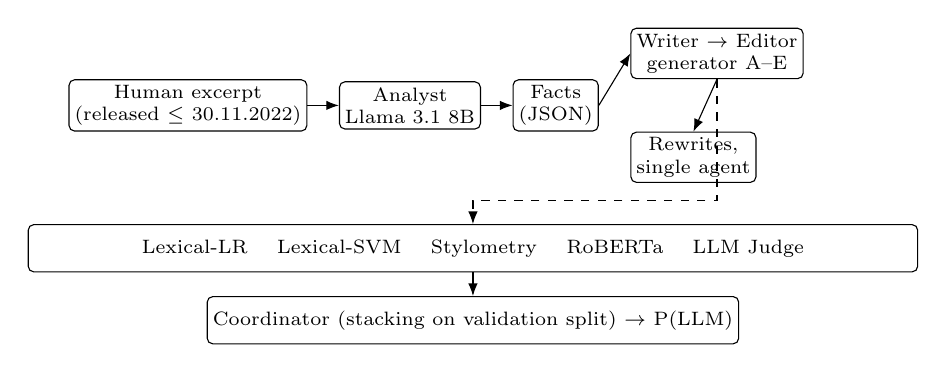
\begin{tikzpicture}[
  box/.style={draw, rounded corners=2pt, align=center, font=\scriptsize, minimum height=6mm, inner sep=2pt},
  arr/.style={-{Latex[length=1.6mm]}, thin}]
\node[box] (h) {Human excerpt\\(released $\le$ 30.11.2022)};
\node[box, right=4mm of h] (an) {Analyst\\Llama 3.1 8B};
\node[box, right=4mm of an] (f) {Facts\\(JSON)};
\node[box, above right=0mm and 4mm of f] (w) {Writer $\rightarrow$ Editor\\generator A--E};
\node[box, below right=0mm and 4mm of f] (s) {Rewrites,\\single agent};
\draw[arr] (h) -- (an);
\draw[arr] (an) -- (f);
\draw[arr] (f.east) -- (w.west);
\draw[arr] (w.south) -- (s.north);
\node[box, below=12mm of an, xshift=8mm, text width=0.92\columnwidth]
  (d) {Lexical-LR \quad Lexical-SVM \quad Stylometry \quad RoBERTa \quad LLM Judge};
\node[box, below=3mm of d] (c) {Coordinator (stacking on validation split) $\rightarrow$ P(LLM)};
\draw[arr] (d) -- (c);
\draw[arr, dashed] (w.south) |- ([yshift=3mm]d.north) -- (d.north);
\end{tikzpicture}
\caption{Generation agents (top) and detection agents (bottom). All generators write from the same Analyst facts and
never see the human excerpt. Rewritten versions start from the Writer--Editor output; the single-agent condition
reads the human excerpt directly. Human excerpts come from CISA (training and testing) and from Microsoft and
Mandiant (testing only).}
\label{fig:pipeline}
\end{figure}

Fig.~\ref{fig:pipeline} summarizes the pipeline. Each agent is a role prompt bound to one model. It receives one
message and returns one. The \emph{Analyst} reads a human excerpt and returns the facts it states as JSON with ten
keys (actor, malware, CVEs, TTPs, targets, sectors, indicator types, timeline, impact, mitigations), with the
instruction to leave a key empty when the excerpt says nothing about it. It runs once per excerpt on a local
Llama~3.1~8B with JSON-constrained output at temperature 0.2. For each generator, a \emph{Writer} receives the facts
and a target length equal to that of the human excerpt and writes a CTI text. An \emph{Editor} then receives the
facts and the draft and revises the draft against the facts, with the instruction not to add new ones. The Writer
prompt is one of four templates (SOC bulletin, vendor blog, government advisory, incident report) and the sampling
temperature is 0.7 or 1.0. Both are drawn from a random generator seeded by generator and excerpt, so an
interrupted run resumes with the same choices, and both are stored with every text together with all agent
messages and the model name. A reply that is empty or opens with a refusal is requested again, up to three times,
after which the excerpt is skipped for that generator.

The training generators run locally through Ollama: A, Llama~3.1~8B (Meta); B, Qwen~2.5~7B (Alibaba); and C,
Mistral~7B (Mistral AI). Two larger API models serve only as unseen test generators: D, gpt-oss-120b (OpenAI
weights, Groq API), and E, Gemini~3.1~Flash-Lite (Google API). Their free tiers allow about 200k tokens and 500
requests per day. After an initial unrestricted run we therefore restricted D and E to excerpts whose source falls
in the test split of at least one seed, and to the multi-agent condition. All \NVarChunks{} such excerpts have a D
and an E version. Texts generated before the restriction bring the coverage to \NCoverD{} and \NCoverE{} of all
excerpts. They are never used for training and enter only the corpus statistics. For a fixed \SingleShare{} of the
sources, each local generator also produces a \emph{single-agent} version, one call that reads the human excerpt
and rewrites it. The external excerpts receive LLM versions from A, B and C through the same pipeline.

\subsection{Rewriting, prompt strategies and partial generation}
For every excerpt whose source is in the test split of at least one seed, we derived further LLM texts from the
multi-agent texts of A, B and C (Table~\ref{tab:robustness} lists them). Five conditions rewrite a finished text:
\emph{paraphrase, same model} (the generator rewrites its own text with an instruction to keep every fact, name and
number), \emph{paraphrase, other model} (A's text rewritten by B, B's by C, C's by A), \emph{paraphrase twice} (the
same-model paraphrase paraphrased again), \emph{back-translation} through German, and a \emph{``humanize''} prompt
that asks for the register of an experienced analyst at a national CERT, without first person and without advice
to the reader. Two prompt strategies change the Writer: an \emph{advisory-style} prompt that asks for the
impersonal register of a government advisory, and a \emph{few-shot} prompt that shows two human excerpts taken from
sources that are in no seed's test split. The \emph{Writer-only} condition is the Writer's draft before the Editor,
which measures what the third agent changes. Finally, \emph{partly generated} texts join sentences of a human
excerpt with sentences of its own LLM version so that LLM sentences make up about 25\%, 50\% or 75\% of the words.
The LLM block is placed first or last at random, because RoBERTa reads only the first 256 tokens. In total this
adds \NVarTexts{} LLM texts. We label every partly generated text as LLM. This is a convention: a text with a
quarter of LLM words is mostly human, and ``recall'' on these texts measures how much inserted LLM text a detector
needs before it responds.

We did not build a human-edited set, in which people revise LLM drafts. Simulating such edits with another LLM
would measure LLM rewriting a second time, so we leave this condition to future work and use the sentence-level
mixtures as the closest available proxy (Section~\ref{sec:limits}).

\subsection{Preprocessing and splits}
LLM outputs contain wrapping that is not part of the text: reasoning tags, preambles such as ``Here is the revised
text'', titles, markdown, bullet markers and word-count notes. We remove these and normalize Unicode variants of
dashes and quotes in all texts, human and generated. The effect of this step is measured in an ablation. Texts
under 50 words are dropped.

Splits are made by source report: 70\% of CISA sources for training, 10\% for validation and 20\% for testing,
separately for each seed (42, 123, 2024). Reports that are near-duplicates of a test report are then removed from
training and validation (Section~\ref{sec:leaksetup}). A human excerpt and all of its LLM versions, rewritten or
not, always fall in the same split. Vectorizers, scalers, detectors, the Coordinator, calibrators and thresholds are
fitted on training or validation data only. Test, D, E, rewritten and external texts are only scored.

\section{Detection Agents}\label{sec:agents}
\subsection{Members}
\begin{itemize}
\item \textbf{Lexical-LR} (baseline 1): word 1--2-gram and character 3--5-gram TF-IDF with logistic regression.
\item \textbf{Lexical-SVM} (baseline 2): the same features with a linear SVM, Platt-calibrated.
\item \textbf{Stylometry}: 32 features in five groups (length, lexical diversity including MTLD \cite{McCarthy_2010},
punctuation, repetition, part-of-speech shares) with XGBoost.
\item \textbf{Transformer}: RoBERTa-base \cite{Liu_2019} fine-tuned for three epochs, maximum length 256 tokens.
\item \textbf{LLM Judge}: Gemma~2~9B, a model family not used for generation, asked zero-shot for the probability
that a text is AI-generated.
\end{itemize}

\subsection{Training-free reference detectors}
\emph{Fast-DetectGPT} uses the analytic form of the conditional probability curvature with GPT-Neo~2.7B as both the
sampling and the scoring model \cite{Bao_2024}. \emph{Binoculars} uses the authors' pair, Falcon-7B as observer and
Falcon-7B-Instruct as performer \cite{Hans_2024}. Two 7B models do not fit together on an 8~GB GPU, so both are
loaded in 4-bit precision and run in two passes. The observer's next-token distribution is stored on disk,
truncated to its 64 most probable tokens and renormalized, and the performer pass computes perplexity and
cross-perplexity from it. Without truncation this two-pass computation reproduces the exact score, which we checked
on a small model. The truncation is not harmless. On \NBinoCheck{} randomly chosen texts scored both ways, the
truncated score was higher than the exact one in \BinoHigher{} cases, with a median absolute difference of
\BinoMedDiff{} against a median exact score of \BinoMedScore{}, while the rank correlation between the two was
\BinoRho{}. Our Binoculars scores are therefore shifted but order the texts almost as the exact ones do. Both
methods read at most 512 tokens. They need no training, but their scores are not probabilities. We map them to
probabilities with class-balanced Platt scaling on the validation split of each training set, so that they are
compared with the supervised detectors under the same threshold rules.

\subsection{Coordinator}
The Coordinator is a logistic regression on the logits of the five members' probabilities
(stacked generalization \cite{Wolpert_1992}),
\begin{equation}
P(\text{LLM} \mid x) = \sigma\Big(b + \sum_{m=1}^{5} w_m \log\frac{p_m(x)}{1 - p_m(x)}\Big),
\end{equation}
where $p_m(x)$ is the probability from member $m$ and $\sigma$ the logistic function. The weights $w_m$ and the bias
$b$ are fitted on the validation split of the training generators, which the members have not been trained on.
They are logged per run and reported with the results. To find out why a stack can fall behind its best member, we
evaluate four variants on the same predictions: the unweighted mean of member logits (no learned weights), the
single member with the best validation F1 (selection in place of combination), a stack fitted on validation texts
of local generators that are \emph{not} in the training set (weights learned under a simulated generator shift), and
the stack with the two zero-shot detectors added as members.

\subsection{Why several agents}\label{sec:why}
\emph{Generation.} Splitting fact extraction from writing serves the experiment. When one prompt reads the human
excerpt and rewrites it, as in our single-agent condition, the output keeps names and phrasing of the source, and
different generators keep different amounts of it. Between \OverlapSingleMin{} and \OverlapSingleMax{} of the word
trigrams of a single-agent text also occur in its human excerpt, depending on the generator, against
\OverlapMultiMin{} to \OverlapMultiMax{} for multi-agent texts of the same excerpts, where the remaining overlap
comes from entity names and stock phrases that pass through the facts. Cross-generator differences in the
single-agent condition would thus mix style with copying. With a shared Analyst, the content is fixed across all
five generators and the human wording is never shown to the Writer. The Editor adds a review step, as in human CTI
production, and its effect is measured by the Writer-only condition. The price is three calls per text instead of
one.

\emph{Detection.} The members use different evidence: surface n-grams, distributional statistics of style,
contextual representations, the judgment of an instruction-tuned model and, for the reference detectors, likelihood
under another language model. A generator shift does not affect these equally. A larger generator may match human
length, which removes a stylometric cue, while keeping the lower proper-noun share that the lexical models use. If
member errors are not perfectly correlated, a learned combination can be more accurate than any member. The same
argument says where it should fail. Weights fitted on validation texts of the training generators reward the
member that is most reliable there, and that member need not be the one that transfers best. The variants above
test this directly, and Section~\ref{sec:results} reports when the combination helps and when it does not.

\section{Experimental Design}\label{sec:setup}
\subsection{Scenarios}
One training run is made for every non-empty subset of the local generators (A, B, C, AB, AC, BC, ABC) and every
seed, and each trained model is tested on the test split of every generator. This yields four settings from the
same runs: \emph{E1 in-generator} (train and test on the same generator, plus the pooled ABC model), \emph{E2
cross-generator} (train on one, test on another; the required Human+A $\rightarrow$ Human+B and Human+A
$\rightarrow$ Human+C cases are part of it), \emph{E3 leave-one-out} (train on two, test on the third) and \emph{E4
external generator} (any training set, tested on D or E). Each test set holds the LLM texts of one generator for
the test sources and the human excerpts they were made from, so the classes are balanced.

The same runs score the external publishers and the rewritten texts. \emph{Publisher shift} is measured by the
false positive rate on all Microsoft and Mandiant human excerpts and by recall, F1 and ROC-AUC on those excerpts
paired with their A, B and C versions. \emph{Rewriting and partial generation} are measured by recall on the
derived texts, which is compared with recall on the multi-agent texts of the same excerpts. The single-agent
condition is compared with multi-agent texts of the same model and the same excerpts. Two augmented trainings, with
three seeds each, test whether more varied training data help: ABC plus one external publisher (human and LLM
versions), tested on the other publisher, and ABC plus paraphrased and single-agent texts of the training sources.

\subsection{Metrics and statistics}
We report accuracy, precision, recall, F1, macro-F1, ROC-AUC and PR-AUC as mean $\pm$ standard deviation over three
seeds. Intervals and tests work at the level of source reports. Test sources are resampled with replacement
(2{,}000 bootstrap samples), which gives a 95\% percentile interval for a metric, and for a comparison the metric
difference is recomputed on the same resampled sources for both systems, which gives a paired interval and a
two-sided $p$-value. With 2{,}000 samples the smallest such $p$-value is $2/2001$, so Holm's correction
\cite{Holm_1979} cannot reject anything in a family of more than fifty tests. We therefore pool the runs of a
comparison before testing: one test per detector and target for the in-generator against cross-generator gap, one
per scenario for the Coordinator against RoBERTa, one per condition and detector for the rewriting conditions.
Holm's method is applied within each of these families. Where tests are reported per run or per feature, the
Benjamini-Hochberg procedure \cite{Benjamini_1995} is used. Detectors are also compared on single test sets with
exact McNemar tests, Holm-corrected per detector pair. Linguistic differences are tested with Mann-Whitney U and
Cliff's $\delta$ as the effect size, and distinctive n-grams are ranked with weighted log-odds \cite{Monroe_2008}.
For the unseen generators we also report the false positive rate (human texts flagged) and the false negative rate
(LLM texts missed) separately, next to ROC-AUC and the calibration measures, because F1 mixes two errors whose cost
differs in CTI.

\subsection{Leakage checks}\label{sec:leaksetup}
A split by source id prevents leakage only if each report has exactly one id. For CISA this does not hold. Some
advisories are posted twice, under an advisory code such as AA22-110A and under a descriptive address, or again as
an updated copy, and the collector stored each copy as a source of its own. We therefore compare texts by word
5-gram containment, the share of a text's 5-grams that occur in a single other text, and join two reports into a
group when an excerpt of one reaches a containment of at least \LeakDup{} in an excerpt of the other. The test
split of each seed is kept as drawn, because the test-only generators D and E were written for these excerpts, and
every training or validation report in a group with a test report is removed (\LeakRemovedMin{} to
\LeakRemovedMax{} reports per seed). A group split between training and validation is moved to training
(\LeakMovedMin{} to \LeakMovedMax{} reports). This leaves \LeakTrainMin{} to \LeakTrainMax{} training and
\LeakValMin{} to \LeakValMax{} validation reports per seed, and all results in this paper use these purged splits.
The plain splits and the list of removed reports are kept in the repository.

The purged splits are then checked in four ways. First, every saved prediction file is audited: each scored test row
must come from a source in the test split of its seed. Second, every test text, human or generated, is compared with
all training and validation texts of its seed, under the plain and under the purged splits; a stricter cut of
\LeakStrict{} also flags excerpts that share long passages with a training text without being copies of it. Third,
all main runs are compared with the same runs on the plain splits, which have the same test sets, and recomputed
without the test excerpts above the strict cut. The excerpt and all its LLM texts are removed together, so the test
sets stay paired. Fourth, Lexical-LR and Stylometry are retrained under a split by excerpt, which lets excerpts of one
report fall on both sides (the leakage the source split is meant to prevent), and on the purged splits with shuffled
training labels, which should give chance-level results if no label information reaches the models through features
or preprocessing.

\subsection{Calibration and thresholds}
For each detector and training run we fit three calibrators on the validation split: Platt scaling (logistic
regression on the logit of the score) \cite{Platt_1999}, temperature scaling (a single divisor of the logit chosen by
validation log-loss) \cite{Guo_2017} and isotonic regression \cite{Zadrozny_2002}. Because the Coordinator is itself
fitted on the validation split, its calibrators use out-of-fold stacked scores from a five-fold split grouped by
source. Probability quality is measured on the test sets with the Brier score, the expected calibration error with
15 equal-width bins \cite{Naeini_2015} and the negative log-likelihood, and shown in reliability diagrams
(Fig.~\ref{fig:reliability}).

Five decision rules are compared, all set on validation data: the fixed threshold 0.5; the threshold with the best
validation F1; a \emph{pseudo-unseen} threshold with the best F1 on validation texts of local generators that are
neither in the training set nor the test generator; and two \emph{human-quantile} thresholds, the 99th and 95th
percentiles of validation human scores, which aim at a 1\% or 5\% false positive rate and use no LLM text at all.
The last two rules assume nothing about the generator met at test time. They do assume that human text at test
time scores like CISA validation text, and the external publishers test that assumption.

\subsection{Cost}
Inference time is measured on one laptop RTX~4060 (8~GB) for a fixed sample of test texts, with three repetitions
and nothing else running on the GPU. The LLM judge is timed on a smaller sample. Training time is logged in every
run. The Coordinator's cost is the sum of its members run one after another.

\subsection{Error analysis}\label{sec:errors}
False negatives (LLM texts scored as human) are taken from models trained on one local generator, over all seeds,
because that is where D is missed. False positives (human texts scored as LLM) are taken from the same models for
CISA and from the pooled ABC models for the vendor excerpts, because that is where the false alarms occur. For
every text we compute length, MTLD, type-token ratio, proper-noun and pronoun shares, first-person pronouns
(\emph{we, our, us, ours}), agency names, advice terms, technical identifiers (file names, CVE numbers, addresses,
ATT\&CK identifiers) that the Analyst facts do not contain, and the rate of \emph{cues}: occurrences per 100 words
of the word n-grams among the 30 terms with the largest positive and the 30 with the largest negative weight in
Lexical-LR trained on A (\NCueLlm{} and \NCueHuman{} of them are word n-grams).

Three analyses use these properties. First, each error is assigned to one category by the first rule that applies,
and the share of every category among the errors is reported next to its share among all texts of the same group.
Without the second number a category that merely describes the generator would look like a cause. Second,
misclassified texts are compared with correctly classified ones property by property (Mann-Whitney U, Cliff's
$\delta$, Benjamini-Hochberg), after averaging each text over runs so that a text missed in every run is not counted
nine times. Third, a logistic regression of the error indicator on standardized properties, with standard errors
clustered by source, estimates which properties change the odds of an error when the others are held fixed. One
author defined the rules, and they were not validated by a second annotator.

\section{Results}\label{sec:results}
\begin{table*}[t]
\centering
\footnotesize
\caption{Corpus per source. Medians over multi-agent texts (human excerpts for the first row).}
\label{tab:data}
\begin{tabular}{lrrrrrr}
\toprule
Source & Multi & Single & Words & MTLD & Rep.\ bigram & PROPN \\
\midrule
Human (CISA) & 406 & 0 & 302 & 84 & 0.094 & 0.114 \\
A: Llama 3.1 8B & 406 & 83 & 163 & 90 & 0.065 & 0.050 \\
B: Qwen 2.5 7B & 405 & 83 & 147 & 121 & 0.033 & 0.055 \\
C: Mistral 7B & 406 & 83 & 214 & 132 & 0.039 & 0.059 \\
D: gpt-oss-120b & 248 & 0 & 306 & 199 & 0.029 & 0.049 \\
E: Gemini 3.1 Flash-Lite & 305 & 0 & 300 & 169 & 0.031 & 0.033 \\
\bottomrule
\end{tabular}
\end{table*}

\begin{table*}[t]
\centering
\scriptsize
\caption{Main results before and after purging. Plain split: by source id only, with near-duplicates of some test excerpts in training or validation. Purged: the same test sets, with every training and validation report removed that holds a near-duplicate of a test excerpt (containment of word 5-grams $\geq$ 0.5); all other results in this paper use it. Strict: the purged run without the test excerpts that still reach a containment of 0.2. Mean test-set size: 158 texts, 138 under the strict cut. F1 is mean $\pm$ std over three seeds.}
\label{tab:leakage}
\begin{tabular}{llcccccc}
\toprule
Setting & Detector & \multicolumn{3}{c}{F1} & \multicolumn{3}{c}{ROC-AUC} \\
\cmidrule(lr){3-5}\cmidrule(lr){6-8}
 & & Plain split & Purged & Purged, strict & Plain split & Purged & Purged, strict \\
\midrule
In-generator & Lexical-LR & 0.997$\pm$0.004 & 0.997$\pm$0.004 & 0.996$\pm$0.005 & 1.000 & 1.000 & 1.000 \\
In-generator & RoBERTa & 0.992$\pm$0.003 & 0.991$\pm$0.002 & 0.990$\pm$0.003 & 1.000 & 0.999 & 0.999 \\
In-generator & Coordinator & 0.998$\pm$0.000 & 0.996$\pm$0.001 & 0.996$\pm$0.002 & 1.000 & 1.000 & 1.000 \\
Cross (A--C) & Lexical-LR & 0.966$\pm$0.008 & 0.966$\pm$0.009 & 0.969$\pm$0.008 & 1.000 & 1.000 & 1.000 \\
Cross (A--C) & RoBERTa & 0.990$\pm$0.002 & 0.989$\pm$0.002 & 0.987$\pm$0.002 & 1.000 & 0.999 & 0.998 \\
Cross (A--C) & Coordinator & 0.993$\pm$0.003 & 0.993$\pm$0.005 & 0.993$\pm$0.005 & 1.000 & 1.000 & 1.000 \\
D, one generator & Lexical-LR & 0.329$\pm$0.017 & 0.336$\pm$0.032 & 0.327$\pm$0.051 & 0.979 & 0.976 & 0.976 \\
D, one generator & RoBERTa & 0.859$\pm$0.022 & 0.845$\pm$0.061 & 0.836$\pm$0.056 & 0.982 & 0.984 & 0.983 \\
D, one generator & Coordinator & 0.721$\pm$0.083 & 0.732$\pm$0.089 & 0.716$\pm$0.087 & 0.987 & 0.988 & 0.988 \\
E, one generator & Lexical-LR & 0.961$\pm$0.012 & 0.960$\pm$0.013 & 0.960$\pm$0.014 & 1.000 & 1.000 & 1.000 \\
E, one generator & RoBERTa & 0.991$\pm$0.003 & 0.988$\pm$0.005 & 0.986$\pm$0.005 & 1.000 & 0.999 & 0.999 \\
E, one generator & Coordinator & 0.995$\pm$0.003 & 0.993$\pm$0.010 & 0.992$\pm$0.010 & 1.000 & 1.000 & 1.000 \\
D, ABC & Lexical-LR & 0.883$\pm$0.021 & 0.888$\pm$0.028 & 0.888$\pm$0.035 & 0.987 & 0.985 & 0.984 \\
D, ABC & RoBERTa & 0.958$\pm$0.012 & 0.947$\pm$0.020 & 0.945$\pm$0.018 & 0.990 & 0.987 & 0.986 \\
D, ABC & Coordinator & 0.915$\pm$0.030 & 0.922$\pm$0.048 & 0.918$\pm$0.047 & 0.995 & 0.994 & 0.994 \\
E, ABC & Lexical-LR & 0.993$\pm$0.011 & 0.993$\pm$0.011 & 0.993$\pm$0.012 & 1.000 & 1.000 & 1.000 \\
E, ABC & RoBERTa & 0.979$\pm$0.003 & 0.973$\pm$0.015 & 0.969$\pm$0.018 & 1.000 & 0.999 & 0.999 \\
E, ABC & Coordinator & 0.996$\pm$0.004 & 0.998$\pm$0.004 & 0.998$\pm$0.004 & 1.000 & 1.000 & 1.000 \\
\bottomrule
\end{tabular}
\end{table*}

\begin{table}[t]
\centering
\scriptsize\setlength{\tabcolsep}{3pt}
\caption{Control trainings, F1 at threshold 0.5 (mean over three seeds and the training generators A, B, C). Under the split by excerpt the test sets differ from the main ones, and D and E cover fewer of their excerpts.}
\label{tab:controls}
\begin{tabular}{llcccc}
\toprule
Split & Detector & In & Cross & D & E \\
\midrule
By report, purged (used) & Lexical-LR & 0.997 & 0.966 & 0.336 & 0.960 \\
By report, purged (used) & Stylometry & 0.935 & 0.869 & 0.704 & 0.784 \\
By excerpt (leaky) & Lexical-LR & 0.998 & 0.966 & 0.277 & 0.953 \\
By excerpt (leaky) & Stylometry & 0.929 & 0.865 & 0.677 & 0.782 \\
Purged, labels shuffled & Lexical-LR & 0.507 & 0.526 & 0.480 & 0.442 \\
Purged, labels shuffled & Stylometry & 0.481 & 0.485 & 0.475 & 0.527 \\
\bottomrule
\end{tabular}
\end{table}

\subsection{Leakage checks}\label{sec:leakage}
Under the plain source split the near-duplicate check found leakage. With reports that reuse whole paragraphs, such
as the Hidden Cobra malware reports, \LeakDupSources{} of the \LeakNSources{} sources form \LeakDupGroups{} groups of
near-duplicate reports, and depending on the seed \LeakPlainChunksDupMin{} to \LeakPlainChunksDupMax{} of the
\LeakPlainTestChunksMin{} to \LeakPlainTestChunksMax{} test excerpts (\LeakPlainDupShareMin{} to
\LeakPlainDupShareMax{}) had a human near-duplicate in training or validation, several of them word for word (largest
containment \LeakPlainMaxContainment{}). After purging, no test excerpt has one in any seed
(\LeakPurgedChunksDupMax{} excerpts), and the largest containment of a test text in a training or validation text is
\LeakPurgedMaxContainment{}. Under the strict cut \LeakPurgedChunksStrictMin{} to \LeakPurgedChunksStrictMax{} test
excerpts per seed still share passages with a training text, mostly related advisories and reports of one series
that repeat a background paragraph. No LLM text had a near-duplicate even before purging: when two reports carry the same facts, the Writers
do not reproduce the wording of another text. Excerpts of the same report, which a split by excerpt would separate,
overlap little (median containment \LeakSiblingMedian{}; \LeakSiblingDup{} of \LeakNSiblings{} are near-duplicates),
and no Microsoft or Mandiant excerpt is a near-duplicate of a CISA excerpt (largest containment \LeakVendorMax{}).
The audit of the saved predictions of the purged runs finds no violation. Of the \LeakAuditRows{} scored test rows
in \LeakAuditFiles{} prediction files, \LeakAuditBad{} come from a training or validation source of their seed, and
no source id occurs in two splits of any seed.

Purging changes the results little (Table~\ref{tab:leakage}). Against the runs on the plain splits, with the same
test sets, the F1 of the trained detectors changes by at most \LeakMaxDeltaPurgeFOne{} in any setting and their
ROC-AUC by at most \LeakMaxDeltaPurgeAuc{}. F1 rises in \LeakNUpPurgeFOne{} and falls in \LeakNDownPurgeFOne{} of
the \LeakNCompPurgeFOne{} combinations of trained detector and setting, so the duplicates did not inflate the
results in one direction. On D, where a memorized duplicate could matter most, Lexical-LR has F1
\LeakDLexlrPlain{} on the plain splits and \LeakDLexlrPurged{} on the purged ones, RoBERTa \LeakDTransPlain{} and
\LeakDTransPurged{}. The training-free detectors, whose scores do not depend on the training data and change only
through the Platt mapping on the smaller validation split, move by up to \LeakMaxDeltaZeroPurge{}, so changes of
this size arise from the different validation data alone. Without the test excerpts above the strict cut, F1 changes
by at most \LeakMaxDeltaStrictFOne{} more.

The control trainings agree (Table~\ref{tab:controls}). The split by excerpt, which lets the other excerpts of a test
report into training, does not raise the scores of Lexical-LR (\CtrlChunkInLexlr{} in-generator,
\CtrlChunkCrossLexlr{} across local generators and \CtrlChunkDLexlr{} on D, against \CtrlSourceInLexlr{},
\CtrlSourceCrossLexlr{} and \CtrlSourceDLexlr{} with the purged split). This follows from the design: a human excerpt
and its LLM versions carry the same facts and always share a split, so knowing the content of a report does not tell
the two classes apart. With shuffled training labels both detectors fall to chance (ROC-AUC between
\CtrlShuffledAucMin{} and \CtrlShuffledAucMax{}), so no label information reaches them through the features or the
preprocessing.

\subsection{Linguistic differences}
Table~\ref{tab:data} and Fig.~\ref{fig:boxes} summarize the corpus. Of the \NTests{} generator-feature comparisons,
\NLargeEffects{} show a large effect ($|\delta| \geq 0.474$) after Benjamini-Hochberg correction. Lexical diversity
differs most consistently. The median MTLD is \MedMtldHuman{} for the CISA excerpts and between \MedMtldA{} and
\MedMtldD{} for the generators, and the hapax ratio is higher for every generator ($\delta$ from \HapaxDeltaMin{} to
\HapaxDeltaMax{}). LLM texts repeat fewer bigrams and use fewer proper nouns. The human excerpts name agencies,
products, files and dates again and again, while the generators restate the same facts in general terms. The local
generators also write short texts (median \MedWordsA{}, \MedWordsB{} and \MedWordsC{} words against
\MedWordsHuman{}), whereas D and E match the human length (\MedWordsD{} and \MedWordsE{}). The log-odds ranking
points the same way. LLM texts over-use \emph{our}, \emph{we}, \emph{potential}, \emph{to mitigate} and
\emph{defenders should}, the vocabulary of advice addressed to a reader. The CISA excerpts over-use \emph{CISA},
\emph{FBI}, \emph{see} and \emph{note}, the vocabulary of attribution and cross-reference. H1 holds for all five
generators at the level of single features.

The two vendor publishers sit between CISA and the generators on some of these features. Against CISA, Microsoft
and Mandiant excerpts use more pronouns ($\delta = \PubMicrosoftPosPronDelta$ and $\PubMandiantPosPronDelta$) and
fewer proper nouns ($\delta = \PubMicrosoftPosPropnDelta$ and $\PubMandiantPosPropnDelta$), the direction in which
LLM text differs from CISA. \NPubLarge{} of \NPubTests{} publisher-feature comparisons show a large effect.

\begin{figure*}[t]
\centering
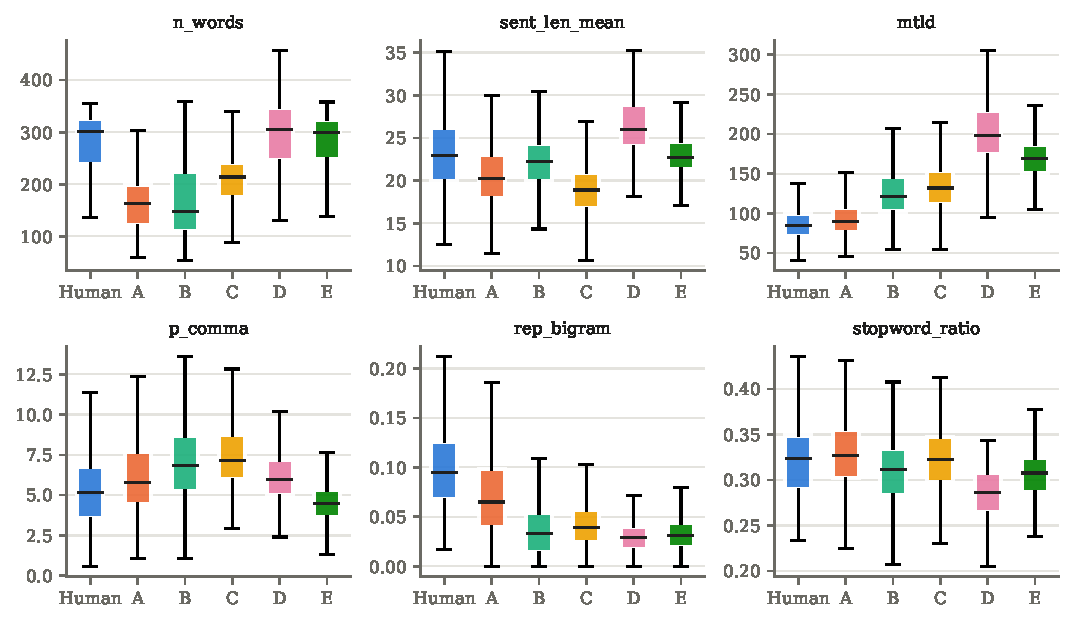
\includegraphics[width=\textwidth]{feature_boxes.pdf}
\caption{Selected stylometric features for CISA excerpts and the five generators (multi-agent texts).}
\label{fig:boxes}
\end{figure*}

\begin{table*}[t]
\centering
\footnotesize
\caption{Models trained on one generator (A, B or C). F1 is mean $\pm$ std over three seeds of the average over training generators; AUC is ROC-AUC.}
\label{tab:main}
\begin{tabular}{lcccccccc}
\toprule
Detector & \multicolumn{2}{c}{In-generator} & \multicolumn{2}{c}{Cross (A--C)} & \multicolumn{2}{c}{D: gpt-oss-120b} & \multicolumn{2}{c}{E: Gemini} \\
 & F1 & AUC & F1 & AUC & F1 & AUC & F1 & AUC \\
\midrule
Lexical-LR & 0.997 $\pm$ 0.004 & 1.000 & 0.966 $\pm$ 0.009 & 1.000 & 0.336 $\pm$ 0.032 & 0.976 & 0.960 $\pm$ 0.013 & 1.000 \\
Lexical-SVM & 0.998 $\pm$ 0.004 & 1.000 & 0.975 $\pm$ 0.004 & 1.000 & 0.351 $\pm$ 0.036 & 0.982 & 0.969 $\pm$ 0.012 & 1.000 \\
Stylometry & 0.935 $\pm$ 0.009 & 0.983 & 0.869 $\pm$ 0.010 & 0.956 & 0.704 $\pm$ 0.010 & 0.875 & 0.784 $\pm$ 0.015 & 0.926 \\
RoBERTa & 0.991 $\pm$ 0.002 & 0.999 & 0.989 $\pm$ 0.002 & 0.999 & 0.845 $\pm$ 0.061 & 0.984 & 0.988 $\pm$ 0.005 & 0.999 \\
LLM Judge & 0.504 $\pm$ 0.024 & 0.409 & 0.504 $\pm$ 0.024 & 0.409 & 0.499 $\pm$ 0.026 & 0.533 & 0.628 $\pm$ 0.015 & 0.754 \\
Fast-DetectGPT & 0.748 $\pm$ 0.004 & 0.828 & 0.729 $\pm$ 0.015 & 0.828 & 0.566 $\pm$ 0.027 & 0.699 & 0.457 $\pm$ 0.019 & 0.613 \\
Binoculars & 0.815 $\pm$ 0.023 & 0.900 & 0.804 $\pm$ 0.016 & 0.900 & 0.390 $\pm$ 0.048 & 0.734 & 0.330 $\pm$ 0.087 & 0.671 \\
Coordinator & 0.996 $\pm$ 0.001 & 1.000 & 0.993 $\pm$ 0.005 & 1.000 & 0.732 $\pm$ 0.089 & 0.988 & 0.993 $\pm$ 0.010 & 1.000 \\
\bottomrule
\end{tabular}
\end{table*}

\subsection{In-generator and cross-generator detection}
Table~\ref{tab:main} gives the main result for models trained on one generator. In-generator detection is close to
perfect for the lexical baselines (F1 \FoneInLexLR{}), RoBERTa (\FoneInTrans{}) and the Coordinator
(\FoneInCoord{}). Moving to another local generator costs little. Lexical-LR falls to \FoneCrossLexLR{} and RoBERTa
to \FoneCrossTrans{}, and leave-one-out training on two generators gives similar values (Lexical-LR \LooLexLR{},
RoBERTa \LooTrans{}). Gemini (E) is detected almost as well by these detectors. The large drop is on gpt-oss-120b
(D). Lexical-LR falls to \FoneDLexLR{} (95\% CI [\FoneDLoLexLR{}, \FoneDHiLexLR{}]) and Lexical-SVM to
\FoneDLexSVM{}, while RoBERTa keeps \FoneDTrans{} ([\FoneDLoTrans{}, \FoneDHiTrans{}]) and the Coordinator
\FoneDCoord{} ([\FoneDLoCoord{}, \FoneDHiCoord{}]). Fig.~\ref{fig:heatmap} shows every training set.

Lexical-LR still ranks the D texts above the human ones (AUC \AucDLexLR{}), but at the fixed threshold it finds
only \ThrDLexlrFixedRecall{} of them. In Fig.~\ref{fig:ecdf} the D scores form a band of their own between the
human excerpts and the local generators, mostly below 0.5, so a lower threshold would separate them from the human
texts. Training on more generators moves the boundary. With two generators Lexical-LR reaches F1
\PoolTwoDLexLR{} on D, and with all three \PoolDLexLR{}. RoBERTa reaches \PoolDTrans{} and the Coordinator
\PoolDCoord{} with three.

The two training-free detectors are well below the supervised ones even in-generator (AUC \AucInFast{} for
Fast-DetectGPT and \AucInBino{} for Binoculars), and their ranking degrades on the larger generators (AUC on D
\AucDFast{} and \AucDBino{}, on E \AucEFast{} and \AucEBino{}). The LLM Judge is close to chance (F1
\FoneInJudge{}). Its in-generator AUC of \AucInJudge{} is below 0.5 because it rates \JudgeHumanFlag{} of the CISA
test excerpts as AI-written, more than it does for the texts of some generators.

\begin{figure*}[t]
\centering
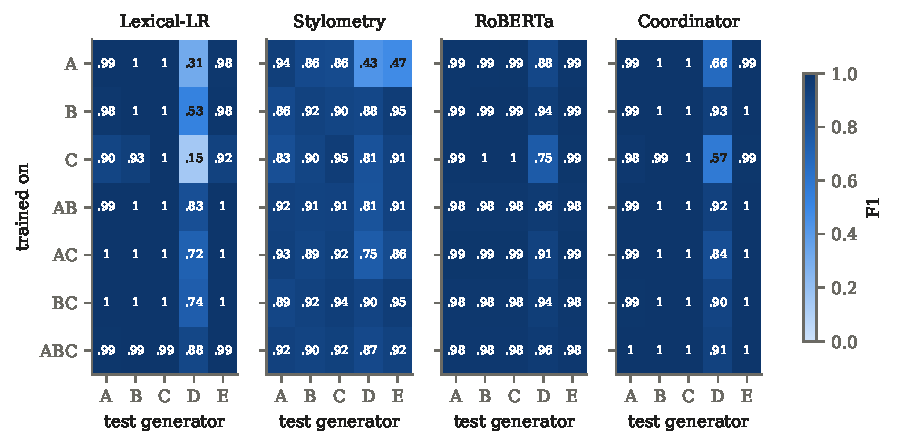
\includegraphics[width=\textwidth]{cross_generator_heatmap.pdf}
\caption{F1 for every training set (rows) and test generator (columns), mean over three seeds. D and E are never
used for training.}
\label{fig:heatmap}
\end{figure*}

\begin{figure}[t]
\centering
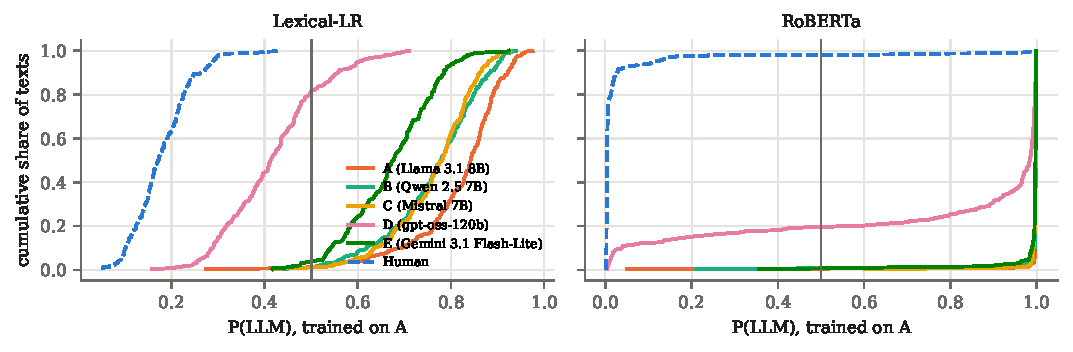
\includegraphics[width=\columnwidth]{score_ecdf.pdf}
\caption{Cumulative distribution of P(LLM) for models trained on A. Human excerpts (dashed) and each generator's
texts; the vertical line is the fixed threshold.}
\label{fig:ecdf}
\end{figure}

\begin{table*}[t]
\centering
\footnotesize
\caption{Training on Human + A, testing on Human + each generator (mean $\pm$ std over seeds).}
\label{tab:required}
\begin{tabular}{llccccccc}
\toprule
Test & Detector & Acc & Precision & Recall & F1 & Macro-F1 & ROC-AUC & PR-AUC \\
\midrule
A & Lexical-LR & 0.994 $\pm$ 0.006 & 1.000 $\pm$ 0.000 & 0.988 $\pm$ 0.013 & 0.994 $\pm$ 0.006 & 0.994 $\pm$ 0.006 & 1.000 $\pm$ 0.000 & 1.000 $\pm$ 0.000 \\
A & RoBERTa & 0.987 $\pm$ 0.006 & 0.980 $\pm$ 0.018 & 0.996 $\pm$ 0.007 & 0.988 $\pm$ 0.006 & 0.987 $\pm$ 0.006 & 0.996 $\pm$ 0.006 & 0.994 $\pm$ 0.011 \\
A & Coordinator & 0.993 $\pm$ 0.007 & 0.991 $\pm$ 0.015 & 0.996 $\pm$ 0.007 & 0.993 $\pm$ 0.007 & 0.993 $\pm$ 0.007 & 1.000 $\pm$ 0.000 & 1.000 $\pm$ 0.000 \\
B & Lexical-LR & 0.996 $\pm$ 0.004 & 1.000 $\pm$ 0.000 & 0.991 $\pm$ 0.008 & 0.996 $\pm$ 0.004 & 0.996 $\pm$ 0.004 & 1.000 $\pm$ 0.000 & 1.000 $\pm$ 0.000 \\
B & RoBERTa & 0.983 $\pm$ 0.009 & 0.979 $\pm$ 0.018 & 0.987 $\pm$ 0.001 & 0.983 $\pm$ 0.009 & 0.983 $\pm$ 0.009 & 0.996 $\pm$ 0.006 & 0.994 $\pm$ 0.010 \\
B & Coordinator & 0.995 $\pm$ 0.008 & 0.991 $\pm$ 0.015 & 1.000 $\pm$ 0.000 & 0.996 $\pm$ 0.008 & 0.995 $\pm$ 0.008 & 1.000 $\pm$ 0.000 & 1.000 $\pm$ 0.000 \\
C & Lexical-LR & 0.994 $\pm$ 0.006 & 1.000 $\pm$ 0.000 & 0.987 $\pm$ 0.013 & 0.994 $\pm$ 0.006 & 0.994 $\pm$ 0.006 & 1.000 $\pm$ 0.000 & 1.000 $\pm$ 0.000 \\
C & RoBERTa & 0.989 $\pm$ 0.009 & 0.980 $\pm$ 0.018 & 1.000 $\pm$ 0.000 & 0.990 $\pm$ 0.009 & 0.989 $\pm$ 0.009 & 0.997 $\pm$ 0.005 & 0.995 $\pm$ 0.008 \\
C & Coordinator & 0.995 $\pm$ 0.008 & 0.991 $\pm$ 0.015 & 1.000 $\pm$ 0.000 & 0.996 $\pm$ 0.008 & 0.995 $\pm$ 0.008 & 1.000 $\pm$ 0.000 & 1.000 $\pm$ 0.000 \\
D & Lexical-LR & 0.595 $\pm$ 0.007 & 1.000 $\pm$ 0.000 & 0.189 $\pm$ 0.015 & 0.318 $\pm$ 0.021 & 0.515 $\pm$ 0.012 & 0.978 $\pm$ 0.020 & 0.978 $\pm$ 0.021 \\
D & RoBERTa & 0.917 $\pm$ 0.018 & 0.977 $\pm$ 0.021 & 0.855 $\pm$ 0.042 & 0.911 $\pm$ 0.021 & 0.917 $\pm$ 0.018 & 0.977 $\pm$ 0.020 & 0.973 $\pm$ 0.028 \\
D & Coordinator & 0.789 $\pm$ 0.101 & 0.979 $\pm$ 0.036 & 0.588 $\pm$ 0.189 & 0.725 $\pm$ 0.156 & 0.777 $\pm$ 0.114 & 0.977 $\pm$ 0.017 & 0.976 $\pm$ 0.023 \\
E & Lexical-LR & 0.981 $\pm$ 0.001 & 1.000 $\pm$ 0.000 & 0.962 $\pm$ 0.002 & 0.981 $\pm$ 0.001 & 0.981 $\pm$ 0.001 & 1.000 $\pm$ 0.000 & 1.000 $\pm$ 0.000 \\
E & RoBERTa & 0.985 $\pm$ 0.008 & 0.979 $\pm$ 0.018 & 0.991 $\pm$ 0.008 & 0.985 $\pm$ 0.007 & 0.985 $\pm$ 0.008 & 0.997 $\pm$ 0.005 & 0.995 $\pm$ 0.007 \\
E & Coordinator & 0.991 $\pm$ 0.010 & 0.991 $\pm$ 0.015 & 0.991 $\pm$ 0.008 & 0.991 $\pm$ 0.010 & 0.991 $\pm$ 0.010 & 0.999 $\pm$ 0.002 & 0.999 $\pm$ 0.002 \\
\bottomrule
\end{tabular}
\end{table*}

Pooled over runs, the F1 lost by moving from the training generator to another local generator is
\HpCrossLexLR{} for Lexical-LR (95\% CI [\HpLoCrossLexLR{}, \HpHiCrossLexLR{}]) and \HpCrossTrans{} for RoBERTa
([\HpLoCrossTrans{}, \HpHiCrossTrans{}]). After Holm correction the loss is significant for \HpSigCross{} of the
\HpNCross{} trained and training-free detectors (Lexical-LR, Lexical-SVM and Stylometry). RoBERTa, the Coordinator
and the two training-free detectors lose no significant F1 between local generators. On D the loss is
\HpDLexLR{} for Lexical-LR, \HpDTrans{} for RoBERTa and \HpDCoord{} for the Coordinator, and it is significant for
all \HpND{} detectors. On E it is significant for \HpSigE{} of \HpNE{}, and neither RoBERTa nor the Coordinator
loses measurably. Tested run by run, \HoneSigCross{} of \HoneNCross{} local comparisons and \HoneSigExt{} of
\HoneNExt{} comparisons on D and E remain significant after Benjamini-Hochberg correction. Exact McNemar tests on
single test sets agree with this picture. After Holm correction RoBERTa differs from Lexical-LR on \McTransLexSig{}
of \McTransLexN{} test sets, the Coordinator from Lexical-LR on \McCoordLexSig{} and the Coordinator from RoBERTa
on \McCoordTransSig{}.

Table~\ref{tab:required} reports every metric for the required setting, training on Human + A, and
Fig.~\ref{fig:cm} shows the Coordinator's confusion matrices for seed 42. On A it makes \CmAFP{} false positives and
\CmAFN{} false negatives (TP \CmATP{}, TN \CmATN{}). On D it still makes \CmDFP{} false positives but misses
\CmDFN{} of \the\numexpr\CmDTP+\CmDFN\relax{} LLM texts. In a CTI pipeline the false negative is the costly error.
A missed fabricated report enters the knowledge base and is shared onward as intelligence, while a false positive
costs an analyst a second look.

\begin{figure*}[t]
\centering
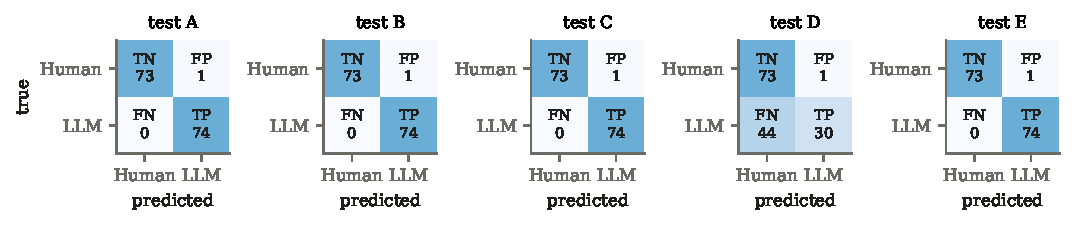
\includegraphics[width=\textwidth]{confusion_coordinator.pdf}
\caption{Coordinator trained on Human + A (seed 42), tested on each generator.}
\label{fig:cm}
\end{figure*}

\begin{table*}[t]
\centering
\footnotesize
\caption{Models trained on CISA + ABC, threshold 0.5. FPR on all human excerpts of the publisher; recall, F1 and AUC on human excerpts paired with their LLM versions from A, B and C, averaged. FPR and F1 are mean $\pm$ std over three seeds; the interval resamples sources. The last column adds the other external publisher to training.}
\label{tab:publishers}
\begin{tabular}{llccrcrc}
\toprule
Publisher & Detector & FPR & 95\% CI & Recall & F1 & ROC-AUC & FPR, other publisher in training \\
\midrule
CISA & Lexical-LR & 0.014$\pm$0.023 & -- & 0.999 & 0.993$\pm$0.011 & 1.000 & -- \\
CISA & RoBERTa & 0.042$\pm$0.007 & -- & 1.000 & 0.979$\pm$0.003 & 1.000 & -- \\
CISA & Coordinator & 0.009$\pm$0.007 & -- & 1.000 & 0.996$\pm$0.004 & 1.000 & -- \\
CISA & Fast-DetectGPT & 0.222$\pm$0.048 & -- & 0.721 & 0.739$\pm$0.029 & 0.828 & -- \\
CISA & Binoculars & 0.093$\pm$0.008 & -- & 0.750 & 0.811$\pm$0.031 & 0.900 & -- \\
Microsoft & Lexical-LR & 0.152$\pm$0.009 & [0.126, 0.177] & 1.000 & 0.930$\pm$0.004 & 1.000 & 0.016$\pm$0.007 \\
Microsoft & RoBERTa & 0.159$\pm$0.029 & [0.134, 0.184] & 1.000 & 0.927$\pm$0.012 & 1.000 & 0.022$\pm$0.004 \\
Microsoft & Coordinator & 0.046$\pm$0.046 & [0.033, 0.061] & 1.000 & 0.978$\pm$0.022 & 1.000 & 0.000$\pm$0.000 \\
Microsoft & Fast-DetectGPT & 0.110$\pm$0.025 & [0.086, 0.134] & 0.874 & 0.880$\pm$0.008 & 0.954 & -- \\
Microsoft & Binoculars & 0.030$\pm$0.007 & [0.017, 0.045] & 0.885 & 0.924$\pm$0.008 & 0.979 & -- \\
Mandiant & Lexical-LR & 0.137$\pm$0.012 & [0.111, 0.166] & 1.000 & 0.936$\pm$0.005 & 1.000 & 0.011$\pm$0.003 \\
Mandiant & RoBERTa & 0.198$\pm$0.041 & [0.162, 0.237] & 1.000 & 0.910$\pm$0.017 & 1.000 & 0.052$\pm$0.023 \\
Mandiant & Coordinator & 0.064$\pm$0.016 & [0.045, 0.086] & 1.000 & 0.969$\pm$0.007 & 1.000 & 0.023$\pm$0.007 \\
Mandiant & Fast-DetectGPT & 0.116$\pm$0.017 & [0.086, 0.150] & 0.825 & 0.848$\pm$0.011 & 0.940 & -- \\
Mandiant & Binoculars & 0.016$\pm$0.006 & [0.003, 0.031] & 0.826 & 0.895$\pm$0.008 & 0.977 & -- \\
\bottomrule
\end{tabular}
\end{table*}

\subsection{Publisher shift}
The models that handle D best raise false alarms on vendor writing (Table~\ref{tab:publishers}). Trained on CISA
and the three local generators, Lexical-LR flags \PubMicrosoftLexlrFpr{} of Microsoft and \PubMandiantLexlrFpr{} of
Mandiant excerpts as LLM-written, against \PubCisaLexlrFpr{} of CISA test excerpts. For RoBERTa the rates are
\PubMicrosoftTransFpr{} and \PubMandiantTransFpr{} against \PubCisaTransFpr{}. The Coordinator is lower
(\PubMicrosoftCoordFpr{} and \PubMandiantCoordFpr{}). On vendor excerpts paired with their own LLM versions all
three still reach an AUC of \PubMicrosoftTransAuc{}, so the vendor human texts are scored above the threshold but
below their LLM versions.

The false alarms grow with the number of generators in training. Lexical-LR trained on one generator flags
\PoolfprOneMicrosoftLexlr{} of Microsoft and \PoolfprOneMandiantLexlr{} of Mandiant excerpts, on two generators
\PoolfprTwoMicrosoftLexlr{} and \PoolfprTwoMandiantLexlr{}, and on three the values above. RoBERTa goes from
\PoolfprOneMicrosoftTrans{} and \PoolfprOneMandiantTrans{} to \PoolfprTwoMicrosoftTrans{} and
\PoolfprTwoMandiantTrans{} with two. The pooling that recovers D in the previous subsection is therefore the same
step that produces the vendor false alarms. A model that has seen three ways of writing LLM text draws a wider
region around ``LLM'', and human text that is unlike CISA falls into it.

Adding one vendor publisher to training removes most of the problem on the other. The false positive rate on
Microsoft falls to \PubMicrosoftLexlrFprAug{} (Lexical-LR), \PubMicrosoftTransFprAug{} (RoBERTa) and
\PubMicrosoftCoordFprAug{} (Coordinator), and on Mandiant to \PubMandiantLexlrFprAug{}, \PubMandiantTransFprAug{}
and \PubMandiantCoordFprAug{}. The training-free detectors behave the other way round. Their false positive rate is
lower on vendor text than on CISA text (Binoculars \PubMicrosoftBinoFpr{} and \PubMandiantBinoFpr{} against
\PubCisaBinoFpr{}; Fast-DetectGPT \PubMicrosoftFastFpr{} and \PubMandiantFastFpr{} against \PubCisaFastFpr{}). A
scoring language model has no notion of CISA's style, so vendor prose does not look unusual to it.
Section~\ref{sec:erranalysis} examines which vendor excerpts are flagged.

\begin{table*}[t]
\centering
\footnotesize
\caption{Recall on LLM texts at threshold 0.5 under rewriting, prompt strategy and partial generation, trained on CISA + ABC (mean $\pm$ std over three seeds). * marks a recall change from the same excerpts before the change with Holm-adjusted p $<$ 0.05 (per detector).}
\label{tab:robustness}
\begin{tabular}{lccccc}
\toprule
Condition & Lexical-LR & RoBERTa & Coordinator & Fast-DetectGPT & Binoculars \\
\midrule
Writer only, no Editor & 0.999$\pm$0.002 & 1.000$\pm$0.000 & 1.000$\pm$0.000 & 0.847$\pm$0.018* & 0.863$\pm$0.041* \\
Paraphrase, same model & 0.999$\pm$0.002 & 1.000$\pm$0.000 & 1.000$\pm$0.000 & 0.612$\pm$0.036* & 0.560$\pm$0.055* \\
Paraphrase, other model & 1.000$\pm$0.000 & 1.000$\pm$0.000 & 1.000$\pm$0.000 & 0.623$\pm$0.045* & 0.594$\pm$0.036* \\
Paraphrase twice & 1.000$\pm$0.000 & 1.000$\pm$0.000 & 1.000$\pm$0.000 & 0.616$\pm$0.033* & 0.586$\pm$0.066* \\
Back-translation & 0.999$\pm$0.002 & 0.989$\pm$0.003* & 0.994$\pm$0.003 & 0.619$\pm$0.026* & 0.516$\pm$0.038* \\
``Humanize'' prompt & 0.999$\pm$0.002 & 0.999$\pm$0.002 & 0.999$\pm$0.002 & 0.676$\pm$0.040* & 0.681$\pm$0.038* \\
Advisory-style prompt & 0.997$\pm$0.005 & 1.000$\pm$0.000 & 1.000$\pm$0.000 & 0.661$\pm$0.054* & 0.640$\pm$0.068* \\
Few-shot human examples & 0.982$\pm$0.005* & 0.972$\pm$0.007* & 0.952$\pm$0.003* & 0.784$\pm$0.051* & 0.791$\pm$0.010 \\
Single agent reading the source & 0.667$\pm$0.116* & 0.733$\pm$0.087* & 0.565$\pm$0.149* & 0.759$\pm$0.028 & 0.676$\pm$0.082* \\
25\% LLM sentences & 0.316$\pm$0.055* & 0.429$\pm$0.082* & 0.161$\pm$0.029* & 0.469$\pm$0.046* & 0.274$\pm$0.048* \\
50\% LLM sentences & 0.850$\pm$0.006* & 0.663$\pm$0.080* & 0.552$\pm$0.067* & 0.634$\pm$0.039* & 0.502$\pm$0.046* \\
75\% LLM sentences & 0.977$\pm$0.002* & 0.875$\pm$0.022* & 0.857$\pm$0.010* & 0.706$\pm$0.025* & 0.669$\pm$0.059* \\
\bottomrule
\end{tabular}
\end{table*}

\subsection{Rewriting, prompt strategy and partial generation}
Rewriting an LLM text with an LLM does not hide it from the trained detectors (Table~\ref{tab:robustness}).
Paraphrasing by the same model, by another model or twice, back-translation and the ``humanize'' prompt all leave
the recall of Lexical-LR, RoBERTa and the Coordinator at \RecBacktranslateTrans{} or above. The Writer-only drafts
are detected as well as the edited texts, so the Editor does not change what these detectors respond to. The
few-shot prompt, which shows two human excerpts to the Writer, lowers recall slightly (Lexical-LR
\RecPromptFewshotLexlr{}, RoBERTa \RecPromptFewshotTrans{}, Coordinator \RecPromptFewshotCoord{}). The
training-free detectors are affected. Paraphrasing lowers the recall of Fast-DetectGPT from
\RecBaseParaphraseSelfFast{} to \RecParaphraseSelfFast{} and that of Binoculars from \RecBaseParaphraseSelfBino{}
to \RecParaphraseSelfBino{}, and back-translation lowers Binoculars to \RecBacktranslateBino{}, as reported for
likelihood-based detectors on general text \cite{Krishna_2023}. Both also detect the Writer's unedited drafts
better than the final texts (\RecWriterOnlyFast{} and \RecWriterOnlyBino{}), so the Editor pass makes the output
less predictable to a scoring model.

Single-agent rewriting, in which the model reads the human excerpt and rewrites it, does hide LLM text. Recall
falls to \RecSingleLexlr{} (Lexical-LR), \RecSingleTrans{} (RoBERTa) and \RecSingleCoord{} (Coordinator), against
\RecBaseSingleLexlr{} on multi-agent texts of the same model and excerpts. The test sets are small, \NSingleTest{}
single-agent texts over the three generators and seeds, which shows in the standard deviations of
Table~\ref{tab:robustness}. These are the texts that share a quarter to a third of their word trigrams with the
source (Section~\ref{sec:why}).

Partly generated texts are the hardest case (Fig.~\ref{fig:mix}). With a quarter of the words from the LLM, recall
is \RecMixTwoFiveLexlr{}, \RecMixTwoFiveTrans{} and \RecMixTwoFiveCoord{}, and with half of them
\RecMixFiveZeroLexlr{}, \RecMixFiveZeroTrans{} and \RecMixFiveZeroCoord{}. For RoBERTa the position of the LLM
block decides. At 50\% it finds \PosMixFiveZeroFirstTrans{} of the texts that begin with the LLM block and
\PosMixFiveZeroLastTrans{} of those that end with it, because it reads only the first 256 tokens. Lexical-LR, which
reads the whole text, finds \PosMixFiveZeroFirstLexlr{} and \PosMixFiveZeroLastLexlr{}. The Coordinator follows
RoBERTa (\PosMixFiveZeroFirstCoord{} and \PosMixFiveZeroLastCoord{}).

\begin{figure}[t]
\centering
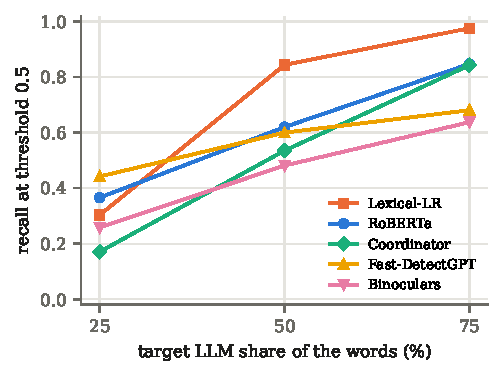
\includegraphics[width=\columnwidth]{mix_recall.pdf}
\caption{Recall on partly generated texts against the share of LLM words, models trained on CISA + ABC.}
\label{fig:mix}
\end{figure}

\begin{table*}[t]
\centering
\footnotesize
\caption{Recall at threshold 0.5 (mean $\pm$ std over three seeds), ABC training (base) against ABC plus single-agent and paraphrased texts of training sources (aug.).}
\label{tab:augmented}
\begin{tabular}{lcccccc}
\toprule
Test & \multicolumn{2}{c}{Lexical-LR} & \multicolumn{2}{c}{RoBERTa} & \multicolumn{2}{c}{Coordinator} \\
 & base & aug. & base & aug. & base & aug. \\
\midrule
A & 0.996$\pm$0.007 & 0.996$\pm$0.007 & 1.000$\pm$0.000 & 1.000$\pm$0.000 & 1.000$\pm$0.000 & 1.000$\pm$0.000 \\
D & 0.801$\pm$0.018 & 0.969$\pm$0.028 & 0.958$\pm$0.030 & 0.995$\pm$0.008 & 0.851$\pm$0.046 & 0.866$\pm$0.087 \\
E & 1.000$\pm$0.000 & 1.000$\pm$0.000 & 1.000$\pm$0.000 & 1.000$\pm$0.000 & 1.000$\pm$0.000 & 1.000$\pm$0.000 \\
Paraphrase, same model & 0.999$\pm$0.002 & 1.000$\pm$0.000 & 1.000$\pm$0.000 & 1.000$\pm$0.000 & 1.000$\pm$0.000 & 1.000$\pm$0.000 \\
Paraphrase twice & 1.000$\pm$0.000 & 1.000$\pm$0.000 & 1.000$\pm$0.000 & 1.000$\pm$0.000 & 1.000$\pm$0.000 & 1.000$\pm$0.000 \\
``Humanize'' prompt & 0.999$\pm$0.002 & 1.000$\pm$0.000 & 1.000$\pm$0.000 & 0.999$\pm$0.002 & 0.999$\pm$0.002 & 0.999$\pm$0.002 \\
Single agent & 0.663$\pm$0.113 & 0.892$\pm$0.051 & 0.721$\pm$0.052 & 0.976$\pm$0.009 & 0.601$\pm$0.121 & 0.766$\pm$0.119 \\
\bottomrule
\end{tabular}
\end{table*}

Training on these conditions helps where the base models failed (Table~\ref{tab:augmented}). Adding paraphrased and
single-agent texts of the training sources raises recall on single-agent test texts from \AugMainSingleLexlr{} to
\AugAugRewriteSingleLexlr{} (Lexical-LR) and from \AugMainSingleTrans{} to \AugAugRewriteSingleTrans{} (RoBERTa),
and on D from \AugMainDLexlr{} to \AugAugRewriteDLexlr{} and from \AugMainDTrans{} to \AugAugRewriteDTrans{},
although no D text was added. The Coordinator gains less (\AugMainSingleCoord{} to \AugAugRewriteSingleCoord{} on
single-agent texts).

\begin{table*}[t]
\centering
\scriptsize\setlength{\tabcolsep}{2.5pt}
\caption{Probability quality on test data, training on one of A, B, C (mean $\pm$ std over three seeds). Calibrators are fitted on validation data only.}
\label{tab:calibration}
\begin{tabular}{@{}ll@{\ }ccccccccc@{}}
\toprule
Detector & Calibrator & \multicolumn{3}{c}{In-generator} & \multicolumn{3}{c}{D: gpt-oss-120b} & \multicolumn{3}{c}{E: Gemini} \\
 & & Brier & ECE & NLL & Brier & ECE & NLL & Brier & ECE & NLL \\
\midrule
Lexical-LR & Raw & 0.035$\pm$0.001 & 0.167$\pm$0.002 & 0.190$\pm$0.002 & 0.201$\pm$0.004 & 0.316$\pm$0.015 & 0.569$\pm$0.009 & 0.073$\pm$0.003 & 0.243$\pm$0.005 & 0.292$\pm$0.008 \\
Lexical-LR & Platt & 0.002$\pm$0.003 & 0.004$\pm$0.002 & 0.014$\pm$0.020 & 0.271$\pm$0.077 & 0.299$\pm$0.075 & 1.823$\pm$0.427 & 0.015$\pm$0.016 & 0.026$\pm$0.019 & 0.054$\pm$0.055 \\
Lexical-LR & Temperature & 0.003$\pm$0.004 & 0.006$\pm$0.005 & 0.025$\pm$0.033 & 0.353$\pm$0.048 & 0.380$\pm$0.023 & 2.899$\pm$1.656 & 0.030$\pm$0.008 & 0.050$\pm$0.012 & 0.135$\pm$0.050 \\
Lexical-LR & Isotonic & 0.003$\pm$0.002 & 0.006$\pm$0.002 & 0.017$\pm$0.019 & 0.242$\pm$0.050 & 0.289$\pm$0.055 & 2.037$\pm$0.524 & 0.015$\pm$0.012 & 0.036$\pm$0.022 & 0.057$\pm$0.047 \\
RoBERTa & Raw & 0.007$\pm$0.003 & 0.013$\pm$0.003 & 0.029$\pm$0.011 & 0.097$\pm$0.010 & 0.113$\pm$0.010 & 0.384$\pm$0.049 & 0.008$\pm$0.003 & 0.016$\pm$0.004 & 0.033$\pm$0.014 \\
RoBERTa & Platt & 0.008$\pm$0.005 & 0.010$\pm$0.005 & 0.059$\pm$0.046 & 0.170$\pm$0.098 & 0.181$\pm$0.096 & 1.772$\pm$1.409 & 0.020$\pm$0.016 & 0.024$\pm$0.015 & 0.202$\pm$0.197 \\
RoBERTa & Temperature & 0.007$\pm$0.002 & 0.014$\pm$0.005 & 0.050$\pm$0.022 & 0.102$\pm$0.010 & 0.114$\pm$0.008 & 0.589$\pm$0.062 & 0.009$\pm$0.003 & 0.017$\pm$0.005 & 0.055$\pm$0.019 \\
RoBERTa & Isotonic & 0.008$\pm$0.005 & 0.010$\pm$0.006 & 0.077$\pm$0.066 & 0.158$\pm$0.094 & 0.177$\pm$0.095 & 1.906$\pm$1.375 & 0.020$\pm$0.014 & 0.026$\pm$0.015 & 0.227$\pm$0.197 \\
Coordinator & Raw & 0.002$\pm$0.000 & 0.005$\pm$0.002 & 0.008$\pm$0.001 & 0.159$\pm$0.043 & 0.203$\pm$0.049 & 0.598$\pm$0.198 & 0.005$\pm$0.003 & 0.021$\pm$0.007 & 0.026$\pm$0.010 \\
Coordinator & Platt & 0.002$\pm$0.001 & 0.004$\pm$0.003 & 0.015$\pm$0.011 & 0.184$\pm$0.067 & 0.202$\pm$0.072 & 1.303$\pm$0.621 & 0.006$\pm$0.002 & 0.011$\pm$0.002 & 0.024$\pm$0.011 \\
Coordinator & Temperature & 0.002$\pm$0.000 & 0.003$\pm$0.002 & 0.015$\pm$0.012 & 0.191$\pm$0.058 & 0.202$\pm$0.053 & 1.916$\pm$0.854 & 0.005$\pm$0.002 & 0.009$\pm$0.003 & 0.035$\pm$0.022 \\
Coordinator & Isotonic & 0.002$\pm$0.000 & 0.004$\pm$0.002 & 0.014$\pm$0.014 & 0.173$\pm$0.055 & 0.208$\pm$0.059 & 1.492$\pm$0.684 & 0.006$\pm$0.003 & 0.015$\pm$0.007 & 0.030$\pm$0.020 \\
\bottomrule
\end{tabular}
\end{table*}

\begin{table*}[t]
\centering
\footnotesize
\caption{Effect of the decision rule, training on one of A, B, C. Every threshold is set on validation data. Pseudo-unseen uses validation texts of local generators that are neither in training nor the test generator. Human 1\% and 5\% use validation human scores alone.}
\label{tab:thresholds}
\begin{tabular}{llccccccc}
\toprule
Detector & Threshold rule & F1, in & F1, cross & F1, D & Recall, D & F1, E & F1, ext. & FPR, ext. \\
\midrule
Lexical-LR & Fixed 0.5 & 0.997$\pm$0.004 & 0.966$\pm$0.008 & 0.329$\pm$0.017 & 0.208 & 0.961$\pm$0.012 & 0.982$\pm$0.001 & 0.003 \\
Lexical-LR & Validation F1 & 0.997$\pm$0.003 & 0.978$\pm$0.019 & 0.502$\pm$0.099 & 0.363 & 0.980$\pm$0.025 & 0.983$\pm$0.005 & 0.016 \\
Lexical-LR & Pseudo-unseen F1 & 0.996$\pm$0.003 & 0.994$\pm$0.003 & 0.758$\pm$0.047 & 0.619 & 0.996$\pm$0.004 & 0.971$\pm$0.001 & 0.058 \\
Lexical-LR & Human 5\% FPR & 0.986$\pm$0.017 & 0.986$\pm$0.016 & 0.886$\pm$0.018 & 0.823 & 0.987$\pm$0.017 & 0.905$\pm$0.019 & 0.212 \\
Lexical-LR & Human 1\% FPR & 0.991$\pm$0.015 & 0.990$\pm$0.014 & 0.852$\pm$0.032 & 0.761 & 0.991$\pm$0.015 & 0.935$\pm$0.031 & 0.139 \\
RoBERTa & Fixed 0.5 & 0.992$\pm$0.003 & 0.990$\pm$0.002 & 0.859$\pm$0.022 & 0.777 & 0.991$\pm$0.003 & 0.960$\pm$0.009 & 0.084 \\
RoBERTa & Validation F1 & 0.992$\pm$0.006 & 0.982$\pm$0.005 & 0.773$\pm$0.171 & 0.685 & 0.979$\pm$0.015 & 0.969$\pm$0.011 & 0.057 \\
RoBERTa & Pseudo-unseen F1 & 0.989$\pm$0.007 & 0.983$\pm$0.006 & 0.819$\pm$0.103 & 0.743 & 0.980$\pm$0.010 & 0.964$\pm$0.012 & 0.071 \\
RoBERTa & Human 5\% FPR & 0.961$\pm$0.031 & 0.961$\pm$0.031 & 0.909$\pm$0.014 & 0.905 & 0.961$\pm$0.031 & 0.901$\pm$0.035 & 0.223 \\
RoBERTa & Human 1\% FPR & 0.980$\pm$0.019 & 0.978$\pm$0.018 & 0.862$\pm$0.065 & 0.807 & 0.977$\pm$0.017 & 0.948$\pm$0.033 & 0.111 \\
Coordinator & Fixed 0.5 & 0.998$\pm$0.000 & 0.993$\pm$0.003 & 0.721$\pm$0.083 & 0.593 & 0.995$\pm$0.003 & 0.989$\pm$0.004 & 0.019 \\
Coordinator & Validation F1 & 0.998$\pm$0.000 & 0.993$\pm$0.003 & 0.708$\pm$0.092 & 0.580 & 0.993$\pm$0.004 & 0.989$\pm$0.004 & 0.018 \\
Coordinator & Pseudo-unseen F1 & 0.992$\pm$0.008 & 0.991$\pm$0.003 & 0.803$\pm$0.087 & 0.705 & 0.992$\pm$0.008 & 0.980$\pm$0.013 & 0.041 \\
Coordinator & Human 5\% FPR & 0.973$\pm$0.019 & 0.973$\pm$0.019 & 0.935$\pm$0.001 & 0.928 & 0.973$\pm$0.019 & 0.918$\pm$0.014 & 0.180 \\
Coordinator & Human 1\% FPR & 0.984$\pm$0.008 & 0.984$\pm$0.009 & 0.892$\pm$0.037 & 0.840 & 0.984$\pm$0.009 & 0.950$\pm$0.014 & 0.107 \\
\bottomrule
\end{tabular}
\end{table*}

\subsection{Calibration and decision thresholds}
In-generator, calibration on validation data improves the probabilities. The expected calibration error of
Lexical-LR falls from \CalLexlrRawInEce{} (raw) to \CalLexlrPlattInEce{} with Platt scaling
(Table~\ref{tab:calibration}). Under generator shift the probabilities get worse. On D, the negative
log-likelihood of Lexical-LR rises from \CalLexlrRawDNll{} (raw) to \CalLexlrPlattDNll{} (Platt) and
\CalLexlrIsotonicDNll{} (isotonic), and that of RoBERTa from \CalTransRawDNll{} to \CalTransPlattDNll{} and
\CalTransIsotonicDNll{}. The calibrators learn from validation data that the scores are reliable and sharpen them,
and on D the sharpened scores are wrong (Fig.~\ref{fig:reliability}). Temperature scaling, which can only soften or
sharpen all scores together, harms RoBERTa least (NLL \CalTransTemperatureDNll{}). The effect on decisions at 0.5
is mixed. Platt scaling moves the boundary of Lexical-LR enough to raise its F1 on D from \CalfoneLexlrRawD{} to
\CalfoneLexlrPlattD{}, and it lowers that of RoBERTa from \CalfoneTransRawD{} to \CalfoneTransPlattD{}. Calibration
on in-distribution data is thus neither a reliable repair for the decision nor a safe one for the probabilities.

\begin{figure*}[t]
\centering
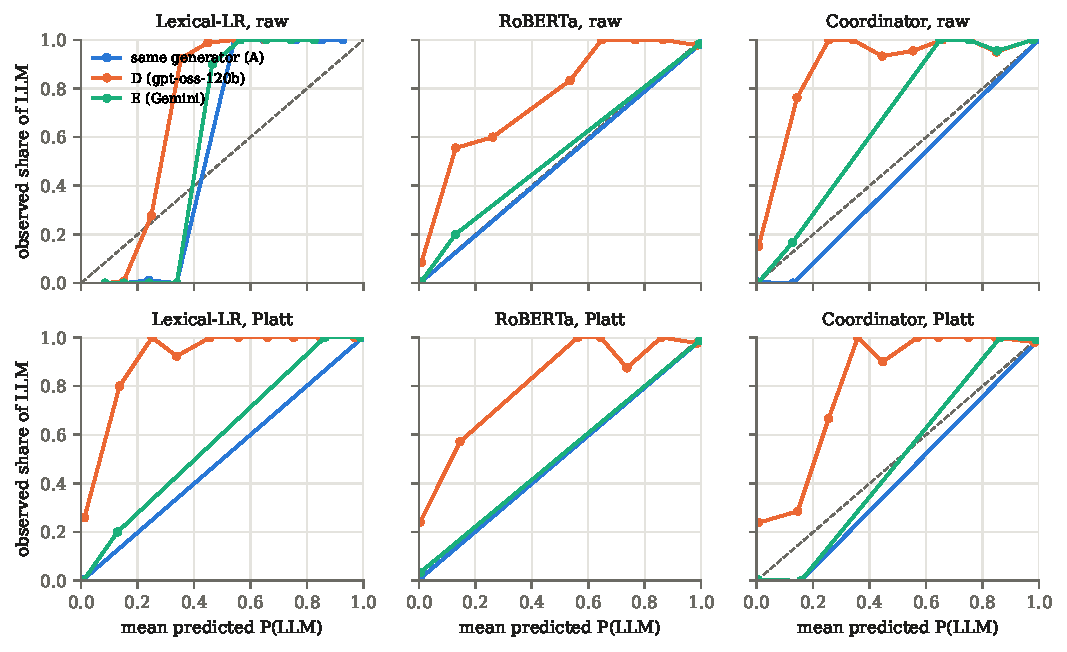
\includegraphics[width=0.9\textwidth]{reliability.pdf}
\caption{Reliability of raw (top) and Platt-scaled (bottom) probabilities, models trained on A. Points are bins with
at least five texts; the dashed diagonal is perfect calibration.}
\label{fig:reliability}
\end{figure*}

The threshold matters more than the calibrator (Table~\ref{tab:thresholds}, Fig.~\ref{fig:sweep}). Choosing the
threshold with the best validation F1 is an unreliable fix, because the validation texts come from the training
generator. It raises Lexical-LR on D only to \ThrDLexlrValfFOne{} and lowers RoBERTa to \ThrDTransValfFOne{}. The
pseudo-unseen rule, which tunes the threshold on another local generator, raises the F1 of Lexical-LR on D from
\ThrDLexlrFixedFOne{} to \ThrDLexlrPseudoFOne{}. The two human-quantile rules, which use no LLM text at all, raise
it to \ThrDLexlrHumoneFOne{} (1\% target) and \ThrDLexlrHumfiveFOne{} (5\% target), and that of the Coordinator
from \ThrDCoordFixedFOne{} to \ThrDCoordHumoneFOne{} and \ThrDCoordHumfiveFOne{}. RoBERTa, whose D scores were
already mostly above 0.5, gains less (\ThrDTransFixedFOne{} to \ThrDTransHumfiveFOne{}).

The cost shows on the other publishers. Table~\ref{tab:thresholds} is computed for models trained on one
generator, which at the fixed threshold flag only \ThrExternalLexlrFixedFpr{} (Lexical-LR) and
\ThrExternalCoordFixedFpr{} (Coordinator) of the vendor excerpts, far fewer than the pooled models of
Table~\ref{tab:publishers}. With the 5\% rule these rates rise to \ThrExternalLexlrHumfiveFpr{} and
\ThrExternalCoordHumfiveFpr{}. Vendor human texts score higher than CISA ones, so a quantile of CISA scores lets
more of them through. Of the five rules, those that recover most of D also raise false alarms on vendor text the
most, which is the trade already seen for pooled training.

\begin{figure}[t]
\centering
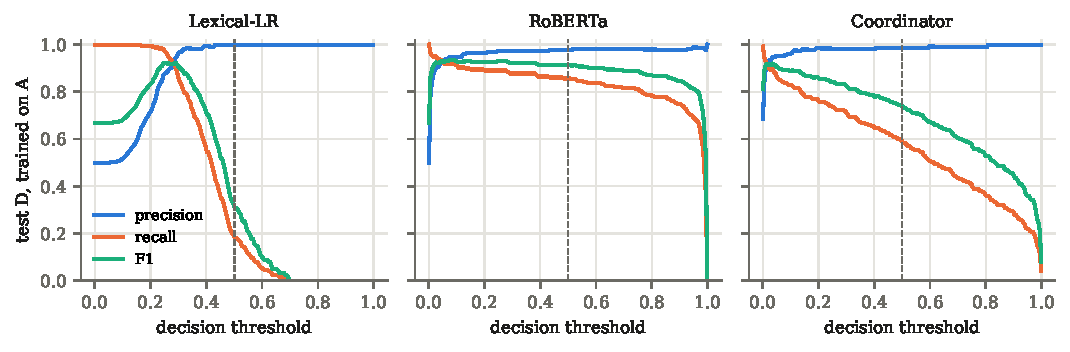
\includegraphics[width=\columnwidth]{threshold_sweep.pdf}
\caption{Precision, recall and F1 on D against the decision threshold, models trained on A; the dashed line is 0.5.}
\label{fig:sweep}
\end{figure}

\begin{table*}[t]
\centering
\scriptsize\setlength{\tabcolsep}{2.5pt}
\caption{Errors, ranking and probability quality on the unseen generators D and E, next to the in-generator reference. FPR is measured on the CISA excerpts of each test set and FNR on the LLM texts. ECE and Brier use the uncalibrated scores. The last two columns use the threshold at the 95th percentile of validation human scores. Mean $\pm$ std over three seeds.}
\label{tab:newgen}
\begin{tabular}{@{}llcccccccc@{}}
\toprule
 & & \multicolumn{6}{c}{Threshold 0.5, raw scores} & \multicolumn{2}{c}{Human 5\% rule} \\
\cmidrule(lr){3-8}\cmidrule(lr){9-10}
Test & Detector & F1 & FPR & FNR & ROC-AUC & ECE & Brier & FPR & FNR \\
\midrule
In-generator & Lexical-LR & 0.997$\pm$0.004 & 0.000$\pm$0.000 & 0.007$\pm$0.009 & 1.000$\pm$0.000 & 0.170$\pm$0.004 & 0.036$\pm$0.002 & 0.028$\pm$0.042 & 0.001$\pm$0.002 \\
In-generator & RoBERTa & 0.991$\pm$0.002 & 0.015$\pm$0.004 & 0.003$\pm$0.005 & 0.999$\pm$0.002 & 0.015$\pm$0.002 & 0.007$\pm$0.001 & 0.049$\pm$0.014 & 0.001$\pm$0.002 \\
In-generator & Coordinator & 0.996$\pm$0.001 & 0.003$\pm$0.005 & 0.004$\pm$0.004 & 1.000$\pm$0.000 & 0.006$\pm$0.000 & 0.002$\pm$0.001 & 0.039$\pm$0.023 & 0.000$\pm$0.000 \\
In-generator & Fast-DetectGPT & 0.748$\pm$0.004 & 0.256$\pm$0.050 & 0.249$\pm$0.027 & 0.828$\pm$0.011 & 0.109$\pm$0.007 & 0.169$\pm$0.007 & 0.124$\pm$0.076 & 0.409$\pm$0.096 \\
In-generator & Binoculars & 0.815$\pm$0.023 & 0.116$\pm$0.022 & 0.229$\pm$0.044 & 0.900$\pm$0.012 & 0.216$\pm$0.022 & 0.221$\pm$0.003 & 0.050$\pm$0.010 & 0.294$\pm$0.032 \\
D, one generator & Lexical-LR & 0.336$\pm$0.032 & 0.000$\pm$0.000 & 0.787$\pm$0.025 & 0.976$\pm$0.011 & 0.311$\pm$0.012 & 0.201$\pm$0.007 & 0.028$\pm$0.042 & 0.203$\pm$0.051 \\
D, one generator & RoBERTa & 0.845$\pm$0.061 & 0.015$\pm$0.004 & 0.230$\pm$0.078 & 0.984$\pm$0.013 & 0.120$\pm$0.032 & 0.104$\pm$0.032 & 0.049$\pm$0.014 & 0.071$\pm$0.049 \\
D, one generator & Coordinator & 0.732$\pm$0.089 & 0.003$\pm$0.005 & 0.395$\pm$0.106 & 0.988$\pm$0.008 & 0.209$\pm$0.048 & 0.161$\pm$0.048 & 0.039$\pm$0.023 & 0.062$\pm$0.041 \\
D, one generator & Fast-DetectGPT & 0.566$\pm$0.027 & 0.256$\pm$0.050 & 0.500$\pm$0.046 & 0.699$\pm$0.039 & 0.175$\pm$0.038 & 0.243$\pm$0.020 & 0.124$\pm$0.076 & 0.717$\pm$0.114 \\
D, one generator & Binoculars & 0.390$\pm$0.048 & 0.116$\pm$0.022 & 0.720$\pm$0.046 & 0.734$\pm$0.021 & 0.142$\pm$0.012 & 0.241$\pm$0.001 & 0.050$\pm$0.010 & 0.873$\pm$0.023 \\
D, ABC & Lexical-LR & 0.888$\pm$0.028 & 0.014$\pm$0.023 & 0.191$\pm$0.031 & 0.985$\pm$0.011 & 0.255$\pm$0.001 & 0.119$\pm$0.007 & 0.031$\pm$0.028 & 0.146$\pm$0.036 \\
D, ABC & RoBERTa & 0.947$\pm$0.020 & 0.055$\pm$0.032 & 0.052$\pm$0.026 & 0.987$\pm$0.005 & 0.050$\pm$0.015 & 0.047$\pm$0.018 & 0.047$\pm$0.022 & 0.060$\pm$0.023 \\
D, ABC & Coordinator & 0.922$\pm$0.048 & 0.005$\pm$0.008 & 0.138$\pm$0.078 & 0.994$\pm$0.005 & 0.082$\pm$0.034 & 0.053$\pm$0.030 & 0.039$\pm$0.037 & 0.034$\pm$0.006 \\
D, ABC & Fast-DetectGPT & 0.590$\pm$0.017 & 0.260$\pm$0.063 & 0.474$\pm$0.027 & 0.699$\pm$0.039 & 0.164$\pm$0.013 & 0.241$\pm$0.019 & 0.124$\pm$0.076 & 0.717$\pm$0.114 \\
D, ABC & Binoculars & 0.421$\pm$0.064 & 0.106$\pm$0.019 & 0.703$\pm$0.057 & 0.734$\pm$0.021 & 0.147$\pm$0.040 & 0.236$\pm$0.001 & 0.050$\pm$0.010 & 0.873$\pm$0.023 \\
E, one generator & Lexical-LR & 0.960$\pm$0.013 & 0.000$\pm$0.000 & 0.075$\pm$0.024 & 1.000$\pm$0.000 & 0.245$\pm$0.007 & 0.074$\pm$0.004 & 0.028$\pm$0.042 & 0.000$\pm$0.000 \\
E, one generator & RoBERTa & 0.988$\pm$0.005 & 0.015$\pm$0.004 & 0.009$\pm$0.012 & 0.999$\pm$0.002 & 0.018$\pm$0.004 & 0.010$\pm$0.004 & 0.049$\pm$0.014 & 0.002$\pm$0.003 \\
E, one generator & Coordinator & 0.993$\pm$0.010 & 0.003$\pm$0.005 & 0.012$\pm$0.014 & 1.000$\pm$0.001 & 0.023$\pm$0.010 & 0.007$\pm$0.007 & 0.039$\pm$0.023 & 0.000$\pm$0.000 \\
E, one generator & Fast-DetectGPT & 0.457$\pm$0.019 & 0.256$\pm$0.050 & 0.625$\pm$0.020 & 0.613$\pm$0.043 & 0.218$\pm$0.018 & 0.286$\pm$0.013 & 0.124$\pm$0.076 & 0.831$\pm$0.125 \\
E, one generator & Binoculars & 0.330$\pm$0.087 & 0.116$\pm$0.022 & 0.771$\pm$0.072 & 0.671$\pm$0.050 & 0.102$\pm$0.038 & 0.244$\pm$0.003 & 0.050$\pm$0.010 & 0.893$\pm$0.032 \\
E, ABC & Lexical-LR & 0.993$\pm$0.011 & 0.014$\pm$0.023 & 0.000$\pm$0.000 & 1.000$\pm$0.000 & 0.193$\pm$0.006 & 0.048$\pm$0.003 & 0.031$\pm$0.028 & 0.000$\pm$0.000 \\
E, ABC & RoBERTa & 0.973$\pm$0.015 & 0.055$\pm$0.032 & 0.000$\pm$0.000 & 0.999$\pm$0.001 & 0.035$\pm$0.011 & 0.027$\pm$0.012 & 0.047$\pm$0.022 & 0.000$\pm$0.000 \\
E, ABC & Coordinator & 0.998$\pm$0.004 & 0.005$\pm$0.008 & 0.000$\pm$0.000 & 1.000$\pm$0.000 & 0.008$\pm$0.007 & 0.002$\pm$0.003 & 0.039$\pm$0.037 & 0.000$\pm$0.000 \\
E, ABC & Fast-DetectGPT & 0.458$\pm$0.015 & 0.260$\pm$0.063 & 0.625$\pm$0.023 & 0.613$\pm$0.043 & 0.216$\pm$0.027 & 0.285$\pm$0.013 & 0.124$\pm$0.076 & 0.831$\pm$0.125 \\
E, ABC & Binoculars & 0.323$\pm$0.121 & 0.106$\pm$0.019 & 0.781$\pm$0.103 & 0.671$\pm$0.050 & 0.095$\pm$0.045 & 0.241$\pm$0.004 & 0.050$\pm$0.010 & 0.893$\pm$0.032 \\
\bottomrule
\end{tabular}
\end{table*}

\subsection{Error rates and probability quality on the new generators}\label{sec:newgen}
Table~\ref{tab:newgen} gives the false positive rate, the false negative rate, ROC-AUC and the calibration measures
for D and E side by side. Read together, they separate three cases.

\emph{D after training on one generator: the order holds, the threshold fails.} The trained detectors err in one
direction only. Their false positive rate on the CISA excerpts of the D test sets is the in-generator one
(Lexical-LR \NgDLexlrFpr{}, RoBERTa \NgDTransFpr{}, Coordinator \NgDCoordFpr{}), since these are the same human
texts, while the false negative rate rises from at most \NgInLexlrFnr{} in-generator to \NgDLexlrFnr{},
\NgDTransFnr{} and \NgDCoordFnr{}. ROC-AUC stays between \NgDLexlrRocAuc{} and \NgDCoordRocAuc{}. The D texts are
still scored above the human excerpts, but many of them below 0.5. The probabilities record this shift. The ECE of
RoBERTa grows from \NgInTransEce{} to \NgDTransEce{} and its Brier score from \NgInTransBrier{} to
\NgDTransBrier{}. Lexical-LR has a high ECE already in-generator (\NgInLexlrEce{}), where it makes almost no errors,
because its raw probabilities are cautious: they fall on the correct side of 0.5 but far from 0 and 1. ECE alone
therefore does not show whether a detector errs. Its Brier score, which grows from \NgInLexlrBrier{} to
\NgDLexlrBrier{}, does. Because the order is kept, a threshold from validation human scores recovers most of the
misses. With the 5\% rule the false negative rate on D falls to \NgDLexlrFnrFive{} for Lexical-LR,
\NgDTransFnrFive{} for RoBERTa and \NgDCoordFnrFive{} for the Coordinator, at a false positive rate on CISA text of
\NgDLexlrFprFive{} to \NgDTransFprFive{}. Its cost on vendor text is given in Table~\ref{tab:thresholds}.

\emph{Training-free detectors: the order is lost.} Fast-DetectGPT and Binoculars already flag \NgInFastFpr{} and
\NgInBinoFpr{} of the CISA excerpts in-generator, and on D their ROC-AUC falls to \NgDFastRocAuc{} and
\NgDBinoRocAuc{}. A new threshold cannot repair this. With the 5\% rule their false negative rate on D rises to
\NgDFastFnrFive{} and \NgDBinoFnrFive{}. E is as hard for them as D (ROC-AUC \NgEFastRocAuc{} and \NgEBinoRocAuc{}).

\emph{E: no failure for the trained detectors.} RoBERTa and the Coordinator keep a false negative rate close to the
in-generator one (\NgETransFnr{} and \NgECoordFnr{}), an ROC-AUC of \NgETransRocAuc{} and an ECE of \NgETransEce{}
and \NgECoordEce{}. Lexical-LR misses \NgELexlrFnr{} of the E texts after training on one generator and
\NgEAbcLexlrFnr{} after training on ABC.

Pooled training acts on D like a lower threshold. Trained on ABC, RoBERTa misses \NgDAbcTransFnr{} of the D texts
and its ECE falls to \NgDAbcTransEce{}, while its false positive rate on CISA rises from \NgDTransFpr{} to
\NgDAbcTransFpr{} and on vendor text to the rates of Table~\ref{tab:publishers}. In a CTI pipeline the first case is
the dangerous one. At the fixed threshold a detector trained on one generator lets most reports written by D
through, while its alarm rate on human reports stays where it was, so watching the alarm rate would not reveal the
failure. Since the order is kept, moving the threshold restores most of the recall. A loss of order, as for the
training-free detectors, cannot be repaired this way.

\begin{table*}[t]
\centering
\footnotesize\setlength{\tabcolsep}{3pt}
\caption{F1 of RoBERTa, the Coordinator and its variants at threshold 0.5 in all scenarios (mean over runs; $\pm$ std over seeds for the first two). Gap is Coordinator minus RoBERTa, with a paired source-level bootstrap interval; * marks Holm-adjusted p $<$ 0.05. ``Unseen stack'' fits the Coordinator on validation texts of generators absent from training. ``Multi-agent, same sources'' is the reference for the single-agent row.}
\label{tab:coordinator}
\begin{tabular}{@{}lcccccccc@{}}
\toprule
Scenario & RoBERTa & Coord. & Gap & 95\% CI & Best on val. & Mean logit & Unseen stack & + zero-shot \\
\midrule
In-generator & 0.991$\pm$0.002 & 0.996$\pm$0.001 & +0.005* & [+0.001, +0.010] & 0.997 & 0.998 & 0.997 & 0.996 \\
Cross, local & 0.989$\pm$0.002 & 0.993$\pm$0.005 & +0.004 & [+0.000, +0.008] & 0.973 & 0.994 & 0.994 & 0.992 \\
Leave-one-out & 0.975$\pm$0.006 & 0.994$\pm$0.002 & +0.018* & [+0.011, +0.026] & 0.991 & 0.995 & -- & 0.994 \\
D, one generator & 0.845$\pm$0.061 & 0.732$\pm$0.089 & -0.113* & [-0.137, -0.089] & 0.388 & 0.747 & 0.811 & 0.736 \\
D, ABC & 0.947$\pm$0.020 & 0.922$\pm$0.048 & -0.024 & [-0.052, +0.002] & 0.796 & 0.965 & -- & 0.920 \\
E, one generator & 0.988$\pm$0.005 & 0.993$\pm$0.010 & +0.005 & [-0.001, +0.010] & 0.966 & 0.997 & 0.996 & 0.991 \\
E, ABC & 0.973$\pm$0.015 & 0.998$\pm$0.004 & +0.024* & [+0.011, +0.039] & 0.989 & 0.996 & -- & 0.998 \\
Microsoft, ABC & 0.909$\pm$0.046 & 0.978$\pm$0.010 & +0.069* & [+0.063, +0.075] & 0.952 & 0.954 & -- & 0.981 \\
Mandiant, ABC & 0.901$\pm$0.054 & 0.970$\pm$0.016 & +0.069* & [+0.062, +0.076] & 0.958 & 0.935 & -- & 0.972 \\
Writer only, ABC & 0.973$\pm$0.015 & 0.998$\pm$0.004 & +0.024* & [+0.017, +0.033] & 0.989 & 0.996 & -- & 0.998 \\
Paraphrase, ABC & 0.973$\pm$0.015 & 0.998$\pm$0.004 & +0.025* & [+0.017, +0.032] & 0.988 & 0.996 & -- & 0.998 \\
Paraphrase, other model, ABC & 0.973$\pm$0.015 & 0.998$\pm$0.004 & +0.024* & [+0.017, +0.032] & 0.988 & 0.996 & -- & 0.998 \\
Paraphrase twice, ABC & 0.973$\pm$0.015 & 0.998$\pm$0.004 & +0.025* & [+0.017, +0.032] & 0.988 & 0.996 & -- & 0.998 \\
Back-translation, ABC & 0.968$\pm$0.014 & 0.995$\pm$0.005 & +0.027* & [+0.020, +0.036] & 0.987 & 0.995 & -- & 0.995 \\
Humanize, ABC & 0.973$\pm$0.016 & 0.997$\pm$0.003 & +0.024* & [+0.017, +0.033] & 0.989 & 0.996 & -- & 0.997 \\
Advisory-style prompt, ABC & 0.974$\pm$0.014 & 0.998$\pm$0.004 & +0.024* & [+0.016, +0.032] & 0.987 & 0.995 & -- & 0.998 \\
Few-shot prompt, ABC & 0.959$\pm$0.018 & 0.973$\pm$0.005 & +0.014* & [+0.004, +0.024] & 0.969 & 0.979 & -- & 0.974 \\
Multi-agent, same sources, ABC & 0.994$\pm$0.010 & 1.000$\pm$0.000 & +0.006 & [+0.000, +0.012] & 0.994 & 1.000 & -- & 1.000 \\
Single-agent, ABC & 0.816$\pm$0.084 & 0.694$\pm$0.137 & -0.122* & [-0.168, -0.082] & 0.694 & 0.764 & -- & 0.700 \\
25\% LLM, ABC & 0.574$\pm$0.065 & 0.274$\pm$0.044 & -0.300* & [-0.341, -0.261] & 0.356 & 0.408 & -- & 0.271 \\
50\% LLM, ABC & 0.770$\pm$0.043 & 0.705$\pm$0.057 & -0.064* & [-0.088, -0.043] & 0.730 & 0.790 & -- & 0.708 \\
75\% LLM, ABC & 0.906$\pm$0.003 & 0.920$\pm$0.007 & +0.014 & [+0.001, +0.027] & 0.926 & 0.949 & -- & 0.921 \\
\bottomrule
\end{tabular}
\end{table*}

\subsection{When the Coordinator helps}
Table~\ref{tab:coordinator} compares the Coordinator with RoBERTa in all \GapN{} scenarios. RoBERTa is the
reference because it is the member that loses least under shift. In-generator, Lexical-SVM is as good as the
Coordinator (Table~\ref{tab:main}). The Coordinator is better than RoBERTa in \GapWins{} scenarios and worse in
\GapLosses{} (Holm-adjusted $p<0.05$). The gains are small where both are near the ceiling (in-generator
\GapInGenerator{}, leave-one-out \GapLeaveOneOut{}, the paraphrase conditions) and larger on vendor text (Microsoft
\GapMicrosoftAbc{}, Mandiant \GapMandiantAbc{}), where its lower false positive rate counts. The losses are the
shifts that change the evidence most: texts with a quarter of LLM words (\GapTwoFiveLlmAbc{}), D after training on
one generator (\GapDOneGenerator{}, 95\% CI [\GapLoDOneGenerator{}, \GapHiDOneGenerator{}]), single-agent texts
(\GapSingleAgentAbc{}) and texts with half LLM words (\GapFiveZeroLlmAbc{}). On D after training on all three it is
also behind (\GapDAbc{}), but not significantly.

On validation data, the stack weights Lexical-SVM (\WgtLexsvm{}) and RoBERTa (\WgtTrans{}) most, then Stylometry
(\WgtStylo{}) and Lexical-LR (\WgtLexlr{}). The LLM Judge gets a negative weight (\WgtJudge{}). On D, the mean
logit of Lexical-SVM collapses, and weighted by its coefficient it accounts for \DropLexsvm{} logit units of the
Coordinator's drop, against \DropTrans{} for RoBERTa and \DropStylo{} for Stylometry. Weights fitted on the training
generator thus put most trust in a member that fails on D. Selecting the single best member on validation does
worse (F1 on D \ScDOneGeneratorBestVal{}; the member chosen most often is \BestValTop{}), the unweighted mean of
logits does slightly better (\ScDOneGeneratorCoordMean{}), and a stack fitted on validation texts of local
generators absent from training does best (\ScDOneGeneratorCoordUnseen{}). None reaches RoBERTa alone
(\ScDOneGeneratorTrans{}). Adding the two zero-shot detectors as members changes little
(\ScDOneGeneratorCoordZero{}). Removing RoBERTa from the Coordinator lowers its F1 on D to \CoordNoTransD{}, and
removing any other member changes it by at most \CoordDropMaxOther{} (Table~\ref{tab:ablation}).

\begin{table*}[t]
\centering
\footnotesize
\caption{Ablations, F1 (mean $\pm$ std over seeds; training on one of A, B, C).}
\label{tab:ablation}
\begin{tabular}{lcccc}
\toprule
Condition & In-generator & Cross (A--C) & D & E \\
\midrule
TF-IDF only (LR) & 0.997 $\pm$ 0.004 & 0.966 $\pm$ 0.008 & 0.329 $\pm$ 0.017 & 0.961 $\pm$ 0.012 \\
Stylometry only (XGB) & 0.934 $\pm$ 0.006 & 0.868 $\pm$ 0.004 & 0.706 $\pm$ 0.013 & 0.778 $\pm$ 0.022 \\
TF-IDF + stylometry (LR) & 0.964 $\pm$ 0.005 & 0.919 $\pm$ 0.010 & 0.735 $\pm$ 0.060 & 0.839 $\pm$ 0.021 \\
LR, no output cleaning & 0.997 $\pm$ 0.004 & 0.965 $\pm$ 0.008 & 0.336 $\pm$ 0.018 & 0.955 $\pm$ 0.012 \\
LR, agency names masked & 0.996 $\pm$ 0.004 & 0.967 $\pm$ 0.008 & 0.349 $\pm$ 0.016 & 0.964 $\pm$ 0.012 \\
RoBERTa, agency names masked & 0.988 $\pm$ 0.004 & 0.986 $\pm$ 0.002 & 0.901 $\pm$ 0.035 & 0.985 $\pm$ 0.007 \\
Stylometry: length only & 0.875 $\pm$ 0.008 & 0.790 $\pm$ 0.004 & 0.482 $\pm$ 0.060 & 0.657 $\pm$ 0.039 \\
Stylometry: lexical only & 0.845 $\pm$ 0.025 & 0.816 $\pm$ 0.024 & 0.863 $\pm$ 0.025 & 0.865 $\pm$ 0.033 \\
Stylometry: punctuation only & 0.823 $\pm$ 0.012 & 0.771 $\pm$ 0.024 & 0.492 $\pm$ 0.055 & 0.590 $\pm$ 0.043 \\
Stylometry: repetition only & 0.800 $\pm$ 0.020 & 0.769 $\pm$ 0.024 & 0.825 $\pm$ 0.020 & 0.775 $\pm$ 0.037 \\
Stylometry: POS only & 0.814 $\pm$ 0.038 & 0.755 $\pm$ 0.036 & 0.777 $\pm$ 0.052 & 0.850 $\pm$ 0.063 \\
Coordinator, all agents & 0.998 $\pm$ 0.000 & 0.993 $\pm$ 0.003 & 0.721 $\pm$ 0.083 & 0.995 $\pm$ 0.003 \\
Coordinator without Lexical-LR & 0.998 $\pm$ 0.000 & 0.993 $\pm$ 0.003 & 0.727 $\pm$ 0.084 & 0.995 $\pm$ 0.003 \\
Coordinator without Lexical-SVM & 0.996 $\pm$ 0.002 & 0.990 $\pm$ 0.008 & 0.784 $\pm$ 0.058 & 0.991 $\pm$ 0.002 \\
Coordinator without LLM Judge & 0.999 $\pm$ 0.001 & 0.993 $\pm$ 0.004 & 0.732 $\pm$ 0.102 & 0.996 $\pm$ 0.004 \\
Coordinator without Stylometry & 0.998 $\pm$ 0.002 & 0.994 $\pm$ 0.001 & 0.722 $\pm$ 0.125 & 0.992 $\pm$ 0.004 \\
Coordinator without RoBERTa & 0.997 $\pm$ 0.003 & 0.972 $\pm$ 0.007 & 0.490 $\pm$ 0.094 & 0.960 $\pm$ 0.006 \\
\bottomrule
\end{tabular}
\end{table*}

\subsection{Ablations}
Masking agency names leaves Lexical-LR almost unchanged (\AblLrMaskedIn{} in-generator, \AblLrMaskedCross{} cross),
so the detectors do not depend on the word \emph{CISA} although it tops the log-odds list. Switching off output
cleaning changes nothing (\AblLrNoCleanIn{}).

The length-matched subset keeps LLM texts within 20\% of the length of their human excerpt. Generator A almost
never writes that long (about \LenAN{} such texts per test split), so we report B and C, with \LenBN{} and
\LenCN{} texts per split. The lexical detectors and RoBERTa are unaffected (Lexical-LR \LenBLexLR{} and
\LenCLexLR{}, RoBERTa \LenBTrans{} and \LenCTrans{}). Stylometry falls from \SameBStylo{} to \LenBStylo{} on B and
from \SameCStylo{} to \LenCStylo{} on C. Length therefore carries part of the stylometric signal for the short
generators, most clearly for B, and these subsets are small. The feature groups give the same answer on a larger
sample. Length and punctuation features reach \AblGroupLengthIn{} and \AblGroupPunctuationIn{} in-generator but
\AblGroupLengthD{} and \AblGroupPunctuationD{} on D, which matches human length, while lexical diversity alone gives
\AblGroupLexicalD{} on D, more than the full stylometric model (\AblStylometryD{}).

Holding one Writer template out of training lowers the recall of Lexical-LR on that template to between
\TplRecallMin{} and \TplRecallMax{}, depending on the template, while its AUC stays at \TplAucMin{}. No single
template is needed to rank the texts, but the templates are not interchangeable at a fixed threshold. Across
topics, recall of the Coordinator on the other local generators stays between \TopicCrossMin{} and
\TopicCrossMax{}. On D it is lowest for vulnerability and APT reports (\TopicDVulnerability{} and \TopicDApt{}) and
highest for the small ``other'' group (\TopicDOther{}).

\begin{table*}[t]
\centering
\footnotesize
\caption{Cost and performance, one training generator. Inference on one RTX 4060 laptop GPU, three repetitions over a fixed sample. The Coordinator cost is the sum of its members run one after another; ``Fit'' excludes the LLM judge, which is not trained.}
\label{tab:cost}
\begin{tabular}{lrrrrcccc}
\toprule
Detector & ms/text & Rel. & GPU MiB & Fit s & F1, in & F1, D & AUC, D & F1, E \\
\midrule
Lexical-LR & 1.7 & 0.60 & -- & 1 & 0.997 & 0.329 & 0.979 & 0.961 \\
Lexical-SVM & 2.0 & 0.72 & -- & 1 & 0.998 & 0.327 & 0.983 & 0.969 \\
Stylometry & 25.6 & 9.27 & -- & 0 & 0.934 & 0.706 & 0.878 & 0.778 \\
RoBERTa & 2.8 & 1.00 & 1269 & 20 & 0.992 & 0.859 & 0.982 & 0.991 \\
LLM Judge & 1136.5 & 410.75 & 16 & -- & 0.504 & 0.499 & 0.533 & 0.628 \\
Fast-DetectGPT & 195.9 & 70.78 & 5771 & -- & 0.744 & 0.540 & 0.699 & 0.427 \\
Binoculars & 725.0 & 262.02 & 5005 & -- & 0.817 & 0.365 & 0.734 & 0.307 \\
Coordinator & 1168.6 & 422.34 & -- & -- & 0.998 & 0.721 & 0.987 & 0.995 \\
\bottomrule
\end{tabular}
\end{table*}

\subsection{Cost}
Inference cost ranges from \MsLexLR{}~ms per text for Lexical-LR to \MsJudge{}~ms for the LLM Judge
(Table~\ref{tab:cost}). RoBERTa needs \MsTrans{}~ms on the GPU, Fast-DetectGPT \MsFast{}~ms and Binoculars
\MsBino{}~ms. Run one member after another, the Coordinator costs \MsCoord{}~ms per text, almost all of it the
Judge. Without the Judge it costs \MsCoordNoJudge{}~ms. The Judge's negative stacking weight and the near-zero
effect of removing it mean that this time buys nothing in our data.

\begin{table*}[t]
\centering
\footnotesize
\caption{Mean text properties by source (multi-agent texts for A--E). First person and agency: share of texts with at least one first-person pronoun or agency name. Cues: occurrences per 100 words of the word n-grams with the largest Lexical-LR weights on each side (model trained on A).}
\label{tab:profile}
\begin{tabular}{lrrrrrrr}
\toprule
Source & Words & MTLD & Proper nouns & First person & Agency named & LLM-side cues & Human-side cues \\
\midrule
Human (CISA) & 279 & 86 & 0.118 & 14\% & 78\% & 0.85 & 6.16 \\
A: Llama 3.1 8B & 161 & 94 & 0.058 & 47\% & 10\% & 7.19 & 2.22 \\
B: Qwen 2.5 7B & 166 & 125 & 0.064 & 39\% & 11\% & 5.57 & 2.59 \\
C: Mistral 7B & 210 & 134 & 0.064 & 61\% & 17\% & 5.19 & 2.92 \\
D: gpt-oss-120b & 294 & 206 & 0.051 & 10\% & 13\% & 2.15 & 3.32 \\
E: Gemini 3.1 Flash-Lite & 279 & 170 & 0.035 & 45\% & 9\% & 3.60 & 2.27 \\
Human (Microsoft) & 312 & 95 & 0.063 & 77\% & 1\% & 1.43 & 3.69 \\
Human (Mandiant) & 295 & 93 & 0.078 & 74\% & 4\% & 1.77 & 3.57 \\
\bottomrule
\end{tabular}
\end{table*}

\begin{table*}[t]
\centering
\footnotesize
\caption{Error categories over all seeds: count and share of the errors of each detector. Categories are mutually exclusive and assigned by the first rule that applies (Section~\ref{sec:errors}); a text counts once per run in which it is misclassified. ``All texts'' is the share of the category among all texts of the group, errors or not, so a category is over-represented among the errors only when its share exceeds this. FN and CISA rows: models trained on one generator; vendor rows: models trained on ABC.}
\label{tab:errors}
\begin{tabular}{llcccc}
\toprule
Error & Category & All texts & Lexical-LR & RoBERTa & Coordinator \\
\midrule
FN, D & impersonal, human length & 76\% & 425 (76\%) & 112 (69\%) & 198 (71\%) \\
FN, D & cites an agency & 11\% & 60 (11\%) & 17 (10\%) & 30 (11\%) \\
FN, D & first person, still missed & 10\% & 44 (8\%) & 16 (10\%) & 22 (8\%) \\
FN, D & unsupported technical detail & 4\% & 30 (5\%) & 17 (10\%) & 28 (10\%) \\
FN, other generators & first person, still missed & 46\% & 47 (32\%) & 3 (17\%) & 10 (37\%) \\
FN, other generators & impersonal, short & 30\% & 43 (29\%) & 1 (6\%) & 2 (7\%) \\
FN, other generators & cites an agency & 7\% & 26 (18\%) & 9 (50\%) & 8 (30\%) \\
FN, other generators & impersonal, human length & 17\% & 30 (20\%) & 5 (28\%) & 7 (26\%) \\
FN, other generators & unsupported technical detail & 0\% & 1 (1\%) & 0 & 0 \\
FP, CISA & first person & 15\% & 0 & 4 (36\%) & 2 (100\%) \\
FP, CISA & few proper nouns & 19\% & 0 & 3 (27\%) & 0 \\
FP, CISA & other & 28\% & 0 & 2 (18\%) & 0 \\
FP, CISA & product vulnerability notice & 9\% & 0 & 2 (18\%) & 0 \\
FP, vendor blogs & first person & 75\% & 174 (89\%) & 255 (90\%) & 58 (83\%) \\
FP, vendor blogs & few proper nouns & 16\% & 22 (11\%) & 23 (8\%) & 12 (17\%) \\
FP, vendor blogs & other & 7\% & 0 & 2 (1\%) & 0 \\
FP, vendor blogs & product vulnerability notice & 2\% & 0 & 2 (1\%) & 0 \\
\bottomrule
\end{tabular}
\end{table*}

\begin{table*}[t]
\centering
\footnotesize
\caption{Properties of misclassified against correctly classified texts: means of the two groups and Cliff's $\delta$ (positive when the misclassified texts have more). A text belongs to the first group when at least half of the runs misclassify it. * marks a Mann-Whitney test with Benjamini-Hochberg adjusted p $<$ 0.05. D: models trained on one generator; vendor excerpts: models trained on ABC.}
\label{tab:contrast}
\begin{tabular}{llcccccc}
\toprule
Group & Property & \multicolumn{2}{c}{Lexical-LR} & \multicolumn{2}{c}{RoBERTa} & \multicolumn{2}{c}{Coordinator} \\
 & & means & $\delta$ & means & $\delta$ & means & $\delta$ \\
\midrule
D texts, missed / caught & Texts & 153 / 38 &  & 30 / 161 &  & 79 / 112 &  \\
 & Words & 301 / 258 & +0.31* & 315 / 288 & +0.18 & 324 / 269 & +0.38* \\
 & MTLD & 203 / 222 & -0.29* & 190 / 210 & -0.31* & 195 / 215 & -0.30* \\
 & Type-token ratio & 0.679 / 0.719 & -0.41* & 0.653 / 0.694 & -0.41* & 0.657 / 0.709 & -0.53* \\
 & Proper-noun share & 0.055 / 0.038 & +0.35* & 0.060 / 0.050 & +0.12 & 0.060 / 0.046 & +0.26* \\
 & Uses first person (share of texts) & 0.08 / 0.18 & -0.11 & 0.13 / 0.09 & +0.04 & 0.09 / 0.11 & -0.02 \\
 & LLM-side cues per 100 words & 1.86 / 3.02 & -0.52* & 1.40 / 2.22 & -0.42* & 1.74 / 2.34 & -0.27* \\
 & Human-side cues per 100 words & 1.86 / 1.52 & +0.18 & 2.04 / 1.74 & +0.13 & 1.88 / 1.72 & +0.05 \\
 & Identifiers not in the facts & 0.07 / 0.00 & +0.05 & 0.20 / 0.02 & +0.11* & 0.13 / 0.00 & +0.10* \\
Vendor excerpts, flagged / passed & Texts & 65 / 373 &  & 85 / 353 &  & 22 / 416 &  \\
 & Words & 282 / 307 & -0.33* & 297 / 305 & -0.11 & 274 / 305 & -0.32* \\
 & MTLD & 108 / 92 & +0.39* & 111 / 90 & +0.47* & 124 / 93 & +0.70* \\
 & Type-token ratio & 0.587 / 0.556 & +0.42* & 0.588 / 0.554 & +0.40* & 0.618 / 0.557 & +0.66* \\
 & Proper-noun share & 0.070 / 0.070 & -0.00 & 0.060 / 0.073 & -0.24* & 0.054 / 0.071 & -0.28 \\
 & Pronoun share & 0.035 / 0.035 & +0.00 & 0.035 / 0.035 & +0.01 & 0.035 / 0.035 & +0.03 \\
 & First person per 100 words & 1.41 / 0.87 & +0.33* & 1.27 / 0.87 & +0.29* & 1.26 / 0.93 & +0.24 \\
 & LLM-side cues per 100 words & 2.26 / 1.35 & +0.42* & 1.96 / 1.37 & +0.33* & 2.11 / 1.45 & +0.34* \\
 & Human-side cues per 100 words & 2.13 / 2.34 & -0.09 & 2.18 / 2.34 & -0.05 & 2.38 / 2.31 & +0.07 \\
\bottomrule
\end{tabular}
\end{table*}

\begin{table*}[t]
\centering
\footnotesize
\caption{Examples of confident errors (CISA excerpts and LLM output), with the generator, the length and the mean score over the runs that misclassify the text.}
\label{tab:examples}
\begin{tabular}{p{4.2cm}p{12.8cm}}
\toprule
Error & Opening of the text \\
\midrule
FN, Coordinator: unsupported technical detail. Generator D, 341 words, mean P(LLM) 0.01 & Malicious cyber actors have been observed deploying the KONNI malware family in campaigns that rely on a classic spear-phishing attachment workflow (ATT\&CK T1566.001). The initial infection vector typically consists of a malicious Microsoft Office document that contains a Visual Basic for Applications (VBA) macro. When the recipient enables macros, the VBA code executes a chain of actions designed to establish\ldots \\
FN, Coordinator: impersonal, human length. Generator D, 394 words, mean P(LLM) 0.17 & Network defenders should be aware that a growing cohort of opportunistic domain registrants is leveraging newly acquired Internet domains to stage man-in-the-middle (MitM) attacks against private and enterprise networks. These actors typically purchase or hijack domains with little or no apparent malicious intent and then configure the associated DNS records to redirect traffic through infrastructure they control. Because the domains\ldots \\
FN, Lexical-LR: cites an agency. Generator D, 317 words, mean P(LLM) 0.34 & Malicious cyber actors-most likely advanced persistent threat (APT) groups-have been observed exploiting a series of critical VMware vulnerabilities disclosed in early 2022, specifically CVE-2022-22954, CVE-2022-22960, CVE-2022-22972, and CVE-2022-22973. These flaws enable a server-side template injection (SSTI) that can be leveraged to achieve remote code execution (RCE) on affected VMware products and, in many cases, to elevate privileges to the root\ldots \\
FN, RoBERTa: first person, still missed. Generator D, 348 words, mean P(LLM) 0.04 & The recent discovery of a malicious 32-bit Windows executable that uses an RC6-encrypted payload has triggered a review of our defensive posture. The binary encrypts its core components with the RC6 block cipher, which hampers static analysis and delays visibility until decryption occurs at runtime. This approach is designed to evade signature-based detection, making behavioral monitoring and heuristic analysis essential\ldots \\
FP, RoBERTa: first person. CISA, 156 words, mean P(LLM) 0.77 & Symantec and Norton branded antivirus products contain multiple vulnerabilities. Some of these products are in widespread use throughout government and industry. Exploitation of these vulnerabilities could allow a remote attacker to take control of an affected system. The large number of products affected (24 products), across multiple platforms (OSX, Windows, and Linux), and the severity of these vulnerabilities (remote code\ldots \\
FP, RoBERTa: few proper nouns. CISA, 351 words, mean P(LLM) 0.90 & The threat actors in this campaign have been observed employing a variety of tactics, techniques, and procedures (TTPs). The actors use malware implants to acquire legitimate credentials then leverage those credentials to pivot throughout the local environment. NCCIC is aware of several compromises involving the exploitation of system administrators' credentials to access trusted domains as well as the malicious use\ldots \\
\bottomrule
\end{tabular}
\end{table*}

\subsection{Error analysis}\label{sec:erranalysis}
\emph{What the categories show.} Table~\ref{tab:errors} gives the error categories with their base rates. Of the D
texts that Lexical-LR misses, \ErrFnDImpersonalHumanLengthLexlr{} are impersonal and of human length, but so are
\ErrbaseFnDImpersonalHumanLength{} of all D texts. The category describes how D writes and does not single out the
misses. The same holds for D texts that name an agency. Two categories do depart from their base rate. D texts in
the first person are missed less often than the others (Lexical-LR misses \ErrRateFnDFirstPersonStillMissedLexlr{}
of them against \ErrRateFnDImpersonalHumanLengthLexlr{} of the impersonal ones). Texts that contain technical
identifiers absent from the Analyst facts are missed more often. They are \ErrbaseFnDUnsupportedTechnicalDetail{}
of the D texts and \ErrFnDUnsupportedTechnicalDetailTrans{} of RoBERTa's misses, and RoBERTa misses
\ErrRateFnDUnsupportedTechnicalDetailTrans{} of them against \ErrRateFnDImpersonalHumanLengthTrans{} of the
impersonal ones. This group is small (\ErrNFnDUnsupportedTechnicalDetailLexlr{} run-level cases) and the rule is a
pattern match that also fires on harmless expansions (Table~\ref{tab:examples}), so we read it as an indication:
a text that spells out file names and identifiers looks more like a human advisory to these detectors. For the other generators the few misses concentrate on
texts that name an agency (\ErrbaseFnOtherGeneratorsCitesAnAgency{} of the texts,
\ErrFnOtherGeneratorsCitesAnAgencyTrans{} of RoBERTa's misses).

\emph{Missed against caught D texts.} Table~\ref{tab:contrast} compares the D texts that at least half of the runs
miss with the rest (\FnNLexLR{} against \TpNLexLR{} texts for Lexical-LR, \FnNTrans{} against \TpNTrans{} for
RoBERTa). Missed texts are less diverse (type-token ratio $\delta = \FnDeltaLexlrTtr$ for Lexical-LR,
$\FnDeltaTransTtr$ for RoBERTa and $\FnDeltaCoordTtr$ for the Coordinator). For Lexical-LR and the Coordinator they
are also longer ($\delta = \FnDeltaLexlrNWords$ and $\FnDeltaCoordNWords$) and contain more proper nouns
($\delta = \FnDeltaLexlrPosPropn$ and $\FnDeltaCoordPosPropn$). For RoBERTa neither difference is significant on its
own ($\FnDeltaTransNWords$ and $\FnDeltaTransPosPropn$). The largest single contrast for Lexical-LR is the cue rate.
Missed texts carry fewer of the n-grams the model associates with LLM text ($\delta = \FnDeltaLexlrCuesLlm$), while
the difference in human-side n-grams is small and not significant ($\delta = \FnDeltaLexlrCuesHuman$). In the
regression, one standard deviation more length
multiplies the odds of a miss by \OrLexlrNWords{} for Lexical-LR (95\% CI [\OrLoLexlrNWords{},
\OrHiLexlrNWords{}]), \OrTransNWords{} for RoBERTa and \OrCoordNWords{} for the Coordinator. A higher proper-noun
share raises them for Lexical-LR (\OrLexlrPosPropn{}) and the Coordinator (\OrCoordPosPropn{}) and less for
RoBERTa (\OrTransPosPropn{}, [\OrLoTransPosPropn{}, \OrHiTransPosPropn{}]). Held fixed in the regression, length
also raises RoBERTa's odds of a miss, although missed and caught texts do not differ in length on their own. Higher MTLD lowers the odds for all
three (\OrLexlrMtld{}, \OrTransMtld{}, \OrCoordMtld{}). The top row of Fig.~\ref{fig:errbins} shows the same
relations as miss rates by tertile.

\begin{figure*}[t]
\centering
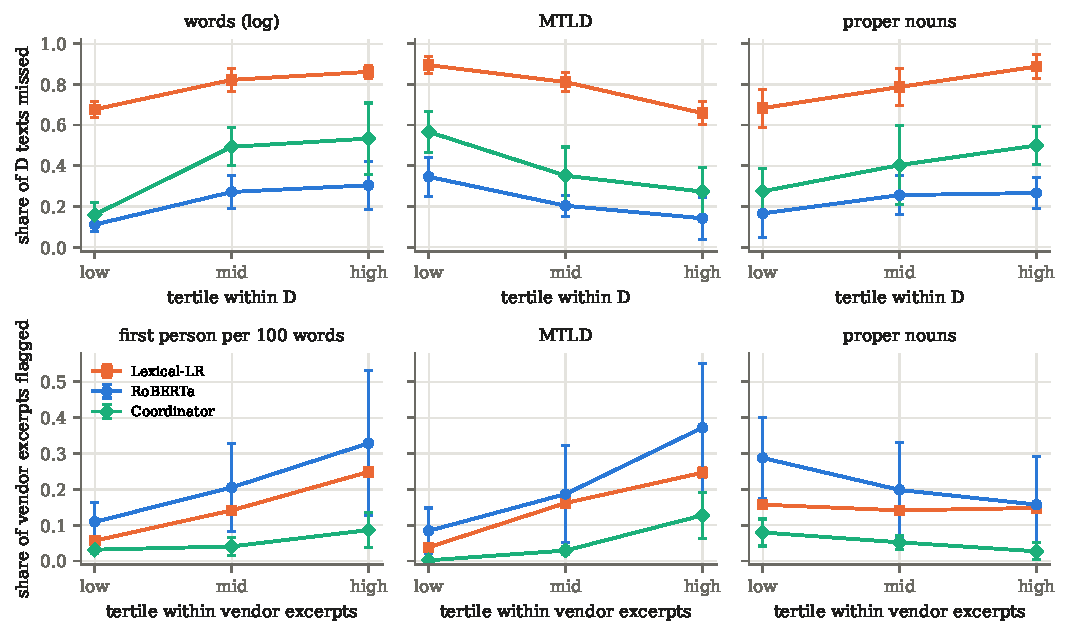
\includegraphics[width=0.92\textwidth]{error_by_bin.pdf}
\caption{Error rate by tertile of a text property (mean and standard deviation over seeds). Top: share of D texts
missed by models trained on one generator. Bottom: share of Microsoft and Mandiant human excerpts flagged by models
trained on ABC.}
\label{fig:errbins}
\end{figure*}

\emph{Why D is missed and E is not.} D and E are both large models and both match the human length, so length does
not explain the difference between them. Table~\ref{tab:profile} points to voice and vocabulary. First-person
pronouns occur in \ProfpctDFirst{} of the D texts, fewer than in the CISA excerpts (\ProfpctHumanFirst{}), and in
\ProfpctEFirst{} of the E texts, which is the range of the local generators (\ProfpctBFirst{} to
\ProfpctCFirst{}). The n-grams that Lexical-LR weights towards LLM occur \ProfDCuesLlm{} times per 100 words in D,
\ProfECuesLlm{} in E and between \ProfCCuesLlm{} and \ProfACuesLlm{} in the local generators (CISA:
\ProfHumanCuesLlm{}). E
writes at human length but keeps the \emph{we} and \emph{our} of the smaller models and their advice vocabulary,
and a detector trained on those models recognizes it. D writes impersonally, repeats identifiers and does not
address the reader. What still marks it as LLM text is its lexical diversity (median MTLD \MedMtldD{} against
\MedMtldHuman{} for CISA), which is why the lexical-diversity features alone detect D better than the full
stylometric model and why the least diverse D texts are the ones missed. The Writer template matters as well.
Lexical-LR misses \DmissIncidentLexlr{} of the D texts written from the incident-report template and
\DmissSocLexlr{} of those from the SOC-bulletin template, and RoBERTa \DmissBlogTrans{} from the vendor-blog
template against \DmissSocTrans{}. The sampling temperature does not (\DmisstempLowLexlr{} at 0.7 and
\DmisstempHighLexlr{} at 1.0 for Lexical-LR).

\emph{False positives.} On CISA test excerpts Lexical-LR makes no false positive and RoBERTa makes
\ErrtotalFpCisaTrans{} over all runs: \ErrNFpCisaFirstPersonTrans{} excerpts written in the first person,
\ErrNFpCisaProductVulnerabilityNoticeTrans{} product vulnerability notices, \ErrNFpCisaFewProperNounsTrans{} with
few proper nouns and \ErrNFpCisaOtherTrans{} other. These counts are too small for more than a description. The
vendor excerpts give enough cases (\ErrtotalFpVendorsLexlr{} run-level false positives for Lexical-LR,
\ErrtotalFpVendorsTrans{} for RoBERTa, \ErrtotalFpVendorsCoord{} for the Coordinator). Vendor blogs write in the
first person as a rule (\ProfpctMicrosoftFirst{} of Microsoft and \ProfpctMandiantFirst{} of Mandiant excerpts
against \ProfpctHumanFirst{} for CISA), and the first-person category is over-represented among the false alarms
(\ErrFpVendorsFirstPersonLexlr{} for Lexical-LR and \ErrFpVendorsFirstPersonTrans{} for RoBERTa against a base
rate of \ErrbaseFpVendorsFirstPerson{}). Table~\ref{tab:contrast} and the bottom row of Fig.~\ref{fig:errbins}
show which excerpts are flagged. They are more diverse (MTLD $\delta = \FpDeltaLexlrMtld$, $\FpDeltaTransMtld$ and
$\FpDeltaCoordMtld$), use the first person more often per 100 words ($\FpDeltaLexlrFirstRate$ and
$\FpDeltaTransFirstRate$), carry more LLM-side cues ($\FpDeltaLexlrCuesLlm$ and $\FpDeltaTransCuesLlm$) and, for
Lexical-LR and the Coordinator, are shorter ($\FpDeltaLexlrNWords$ and $\FpDeltaCoordNWords$). The overall pronoun
share, which separates vendors from CISA at the corpus level, does not separate flagged from passed vendor excerpts
($\FpDeltaLexlrPosPron$ and $\FpDeltaTransPosPron$), and the proper-noun share does so only for RoBERTa
($\FpDeltaTransPosPropn$). In the regression, one standard deviation more first-person use multiplies the odds of
a false alarm by \FpOrLexlrFirstRate{} for Lexical-LR (95\% CI [\FpOrLoLexlrFirstRate{}, \FpOrHiLexlrFirstRate{}])
and \FpOrTransFirstRate{} for RoBERTa, and one standard deviation more MTLD by \FpOrLexlrMtld{},
\FpOrTransMtld{} and \FpOrCoordMtld{} for the Coordinator.

\emph{Examples.} Table~\ref{tab:examples} shows six confident errors. The first D text is counted as adding an
identifier because it writes \texttt{certutil.exe} where the facts say CertUtil, which shows how coarse that rule
is. The second expands the acronym SVR as ``Federal Security
Service'', the name of a different Russian agency (the FSB), an error of content that a style detector cannot see.
The two CISA false positives are a joint advisory written as \emph{we} and a narrative summary with few names.

Taken together, the two kinds of error are mirror images. The LLM texts that are missed are long, impersonal, rich
in proper nouns and low in lexical diversity, the profile of a CISA excerpt. The human texts that are flagged are
shorter, written in the first person and lexically diverse, the profile of the training generators.

\section{Discussion}\label{sec:discussion}
\subsection{Answers to the research questions}
\emph{Q1, linguistic differences.} LLM CTI has higher lexical diversity, repeats fewer bigrams, names fewer
entities and gives more advice to the reader. Human CTI repeats identifiers and cites other documents. This agrees
with the GLTR observation that generated text avoids the long tail of specific tokens \cite{Gehrmann_2019}. Not all
of these features describe human authorship as such. First-person voice separates CISA from the small generators
and from the vendor blogs alike, so it describes CISA's house style. Lexical diversity is the more general
difference. The three human publishers lie close together on MTLD and generators B to E lie well above them,
while A, the least diverse generator, overlaps with the vendor blogs (Table~\ref{tab:profile}).

\emph{Q2, baselines against the transformer.} In-generator, a TF-IDF baseline is as good as RoBERTa. The difference
appears under shift. On D, RoBERTa keeps an F1 of \FoneDTrans{} against \FoneDLexLR{}, and it does not need agency
names to do so (\AblTransformerMaskedD{} with names masked). Pre-trained representations seem to capture properties
of LLM prose beyond the n-grams of the training generators, as the supervised RoBERTa detectors for GPT-2 did
\cite{Solaiman_2019}. The training-free detectors, which need no CTI data, rank texts far worse than any trained
model here. With a 2.7B scoring model and 4-bit 7B models they are weaker than in their authors' settings, and
they are also \RelFast{} and \RelBino{} times slower than RoBERTa.

\emph{Q3 and Q4, generator style and cross-generator testing.} Among the three 7--8B local models, cross-generator
F1 stays near the in-generator value, so the detectors do not learn the style of one model only. Part of what they
learn is specific to how small models write CTI: short, in the first person, with advice to the reader. Gemini
writes longer but keeps that voice and is detected. gpt-oss-120b drops it and is missed by the lexical models,
whose AUC nevertheless stays high. This is the pattern reported by M4 and RAID, where detectors label text from
unseen generators as human \cite{Wang_2024,Dugan_2024}. Our threshold results locate it in the decision, and the
error analysis names the properties involved.

\emph{Q5, important features.} The stylometric model splits mostly on length (top feature: \TopFeature{}) and
proper-noun share, the lexical model on pronouns, hedging words and agency names. The length cue does not transfer
to larger generators. The lexical-diversity cue does, and within D the misses are the long texts with low
diversity and many proper nouns.

\emph{Q6, topics and attack types.} Among local generators recall does not depend on the topic. On D,
vulnerability and APT reports are missed more often than phishing and ransomware reports
(\TopicDVulnerability{} and \TopicDApt{} against \TopicDPhishing{} and \TopicDRansomware{}). A possible reason is
that the facts of such reports are mostly actor, product and CVE names, which raise the proper-noun share of the
generated text. The topic labels come from keyword rules and the standard deviations across runs are large, so we
read this as a tendency.

\emph{Q7, changes in LLM technology.} The detectors trained on 2024-era 7--8B models lose most on the larger and
newer gpt-oss-120b, and they fail on texts produced by a different procedure with the same models, single-agent
rewriting and sentence-level mixing. Paraphrasing affected the two groups of detectors differently. It lowered the
recall of the two likelihood-based detectors, as in general-domain studies \cite{Krishna_2023,Sadasivan_2023}, and
left that of the trained ones unchanged. A plausible reason is that our paraphrasers are the same small
instruction-tuned models. A paraphrase is then another LLM text with the same habits, which a classifier trained on
such texts recognizes even when its token probabilities change. A paraphraser trained to evade detection, as in
RADAR \cite{Hu_2023}, would be a stronger test.

\subsection{Ranking and decision}
Across generator and publisher shift, the supervised detectors kept an AUC near 1 while F1 or the false positive
rate moved. A detector that meets new text can usually still order it, and what fails is the boundary fitted to
the training generators and the training publisher. On D the error rates show this directly
(Table~\ref{tab:newgen}): the false negative rate of the trained detectors rises while their false positive rate
on CISA text and their ROC-AUC stay at the in-generator values. Of the measures that need no threshold, only the
Brier score and ECE register the change. Calibrating on in-distribution validation data does not repair
this, in line with Ovadia et al.\ \cite{Ovadia_2019}. The two repairs that do work for an unseen generator, a
threshold from human scores and training on several generators, both move the boundary towards human text, and
both are paid for on a publisher the model has not seen. The false positive rate of Lexical-LR on Microsoft
excerpts goes from \PoolfprOneMicrosoftLexlr{} to \PoolfprThreeMicrosoftLexlr{} when it is trained on three
generators instead of one. The error analysis says why the two shifts pull in opposite directions. The detectors separate CISA from
the small generators along length, first-person voice and lexical diversity. An unseen generator that sits near
CISA on the first two is missed, and an unseen publisher that sits near the generators on the last two is flagged.
A single boundary on these properties cannot serve both. The remedy that did not have this cost was human text
from more than one publisher. Adding the excerpts of one vendor to training, \NExtChunksMicrosoft{} or
\NExtChunksMandiant{} of them with their LLM versions, cut the false positive rate on the other vendor several
fold.

\subsection{When combining agents helps}
The stacked Coordinator helps when its members fail in different places, as on vendor text, where its false
positive rate is less than half that of Lexical-LR or RoBERTa. It falls behind RoBERTa when the member it trusts
most is the one that fails, as on D after single-generator training. The weights are fitted where all members look
reliable, so the stack cannot know which member will transfer. Learning the weights under a simulated shift
recovers part of the loss, which supports this reading. For a deployment, this suggests choosing the combination
rule on held-out generators and publishers and dropping members, like the LLM Judge here, that add cost and no
signal.

\subsection{Use in a CTI workflow}
For triage of incoming reports, a fine-tuned encoder is the best single choice in our data. On a GPU it is about as
cheap as a TF-IDF model at inference, it keeps most of its recall under generator shift and it is not fooled by
LLM paraphrasing. Its weaknesses are partial generation, where it sees only the first 256 tokens, and false alarms
on unfamiliar publishers. Its score should therefore send a report to an analyst and not block it, long reports
should be scored in windows, and human text from each new source of reports should be added to training before the
detector is trusted on it. Fabricated reports that copy names and identifiers from a real report, as our
single-agent texts do, and reports that mix human and generated paragraphs remain the largest gap.

\section{Limitations and Threats to Validity}\label{sec:limits}
\subsection{Dataset}
\emph{Training publisher.} All training text comes from CISA, so ``human'' in training also means ``this agency's
house style''. The Microsoft and Mandiant sets measure how far that bias carries, but they are vendor blogs
selected by publisher labels and title rules, and \NExtSourcesMicrosoft{} plus \NExtSourcesMandiant{} sources are a
small sample of vendor writing. Other forms of CTI, such as STIX objects, analyst chat or non-English reports, are
not covered. \emph{Size.} \NSources{} CISA sources give test splits of about 40 sources per seed, which is why we
report source-level intervals next to the means. Several subsets are much smaller: the single-agent test texts,
the length-matched subsets and the error categories with a low base rate. \emph{Dates.} Human authorship rests on
publication dates on or before 30 November 2022. CISA pages show revision dates, Microsoft metadata were
overwritten by a site migration and Mandiant posts were moved to a new host, so we date documents by advisory
codes, URL dates and visible bylines and remove paragraphs that announce later updates. A paragraph revised after
the cutoff without such a note would go unnoticed. \emph{Duplicate reports.} The collector treated CISA reposts
of one advisory as separate sources. We found this only after the first full run, in which \LeakPlainDupShareMin{}
to \LeakPlainDupShareMax{} of the test excerpts had a near-duplicate in training or validation, and all results
reported here come from a second run on purged splits (Section~\ref{sec:leakage}). Purging made the validation
splits smaller (\LeakValMin{} to \LeakValMax{} reports). Our check compares word 5-grams and would miss a report that
restates another in new words. \emph{Excluded pages.} \NBlocked{} CISA analysis reports could
not be read because the local antivirus flagged embedded malware samples.

\subsection{Generation}
\emph{Generator coverage.} The three training generators are 7--8B open models from 2024. D and E exist only in
the multi-agent condition and, apart from texts generated before the quota restriction, only for test excerpts, so
we cannot train on larger models or test single-agent rewriting and external publishers with them. The contrast
between D and E rests on one model of each kind. \emph{One pipeline.} All LLM texts come from one set of prompts
and one Analyst. The single-agent and prompt-strategy conditions show that another procedure changes the results.
\emph{Fact drift.} Generators sometimes changed or added facts. Such texts were not filtered, and a reader with
domain knowledge could detect some of them by content. Our measure of added identifiers is a pattern match and
misses invented narrative. \emph{No human-edited texts.} An attacker could have a person revise an LLM draft. We
did not collect such texts, and we chose not to simulate them with another LLM, because that would measure LLM
rewriting again. The sentence-level mixtures approximate a report assembled from human and machine paragraphs, not
a human edit of machine text, and their LLM label is a convention.

\subsection{Detectors and analysis}
\emph{Model choice.} RoBERTa is the only fine-tuned encoder and Gemma~2~9B the only judge, and no hyperparameter
search was done. Binoculars ran in 4-bit precision with a truncated observer distribution, which shifts its
scores, and Fast-DetectGPT with a single 2.7B model. Both are smaller than the strongest settings of their
authors, and Ghostbuster could not be run. \emph{Calibration data.} Calibrators and thresholds come from validation
splits of \LeakValMin{} to \LeakValMax{} sources per seed. A 99th percentile of \LeakValHumanMin{} to
\LeakValHumanMax{} human scores is close to their maximum, and
the 1\% rule realizes false positive rates between \ThrInLexlrHumoneFpr{} and \ThrInTransHumoneFpr{} on CISA test
text.
\emph{Error analysis.} The categories are rule-based, defined by one author and not checked by a second annotator.
The property comparisons and regressions are observational. They show which texts are misclassified and do not
prove that changing a property would change the decision. The cue lists come from one model trained on A.
\emph{Statistics.} Bootstrap intervals resample test sources but treat the three seeds and the training generators
as given, so they do not capture the variance of a different choice of generators. Their $p$-values cannot be
smaller than $2/2001$.

\section{Conclusion}
Human and LLM-written CTI differ in measurable ways, and when the generator is known a TF-IDF model is enough to
separate them. The difficulty starts with text the detector has not seen. In our corpus, where five generators
write from the same extracted facts, the detectors kept ranking such text correctly and lost the decision: a large
unseen generator that writes impersonally was scored below the threshold, and vendor blogs written in the first
person were scored above it. On that generator the errors were false negatives at an unchanged false positive rate,
so the alarm rate gave no warning. These results come from splits purged of near-duplicate reports, and an audit of
the saved predictions confirmed that no test report or copy of one was used in training. Pooling training generators or setting the threshold from human scores repaired the
first failure and aggravated the second, and calibration on validation data repaired neither. Human text from a
second publisher in training was the one remedy without that cost. A stacked combination of detector agents was
worth its cost on vendor text and fell behind RoBERTa where its most trusted member failed. Rewriting an LLM text
with an LLM did not hide it from trained detectors, but rewriting from the source and mixing human with generated
sentences did. The study is limited to one government publisher for training, three small training generators and
one generation pipeline. Human-edited LLM drafts, larger training generators and windowed scoring of long reports
are the next steps.

\section*{Reproducibility}
Code, configuration files, the CISA corpus, all generated texts with every agent message, predictions and result
tables are in the project repository.\footnote{\url{https://github.com/FurkanDevelops/llm-cti-detection}} Every
stage runs from one command, \texttt{python -m src.cli <stage> --config <file>}, and
\texttt{experiments/run\_all.sh} runs them in order. Model names, prompts, sampling temperatures, seeds and
detector settings are in \texttt{configs/}, and package versions are pinned in \texttt{requirements.txt}. Every
number in this paper is written by the report stage into a macro file, so the text cannot drift from the results.
A verify stage checks this. It recomputes every metric from the saved per-text predictions with code independent
of the evaluation stage, rebuilds the macro file and all tables from \texttt{results/}, compares them with the
files this paper was compiled from, and writes a SHA-256 manifest of the result files against which any copy of the
repository can be checked.
The Microsoft and Mandiant excerpts are rebuilt by the collection script from the listed URLs and checked against
stored hashes. API generations (D, E) cannot be repeated exactly, so their outputs are stored.

\bibliographystyle{IEEEtran}
\bibliography{../refs}

\end{document}
